% Лабораторная работа по АСиСу № 1
% Михедов Константин Константинович

% Тип документа: статья, на бумаге А4
\documentclass[a4paper]{article}

% Подключение сторонних tex файлов 
\usepackage{import}


% Основные данные - ВУЗ, факультет, город...
\import{./../../stuff/tex}{config.tex}

% Подключение необходимых зависимостей
\import{./../../stuff/tex/settings}{packages.tex}
% Настройка подключенных пакетов
\import{./../../stuff/tex/settings}{preferences.tex}


% Шаблон титульной страницы 
\import{./../../stuff/tex/templates}{title.tex}
% Упрощенный блок "выполнил"
\import{./../../stuff/tex/templates}{sign1.tex}
% Макрос для содержания
\import{./../../stuff/tex/templates}{toc.tex}

% Определяем название документа
\title{
  Лабораторная работа №2 по курсу \\
  <<Проектный семинар>>  
}
% Отключаем отображение правительства
\renewcommand{\government}{}
% Отключаем сокращенное нзавание университета
\renewcommand{\subuniversity}{}
% Указываем преподавателя
\renewcommand{\shortteachername}{Минченков В.О.}


% Путь до внешних изображений
\graphicspath{ {./figures/}}


% Основной текст работы
\begin{document}
  \templatedtitlepage
  
  \toc
  \section{Ход работы}

  \subsection{DHCP-spoofing}

  В первую очередь настроим сеть для виртуальных машин - укажем адрес сети, маску, включим \textit{DHCP} сервер.
  (Адрес сети и маска установлены в соответсвии с 9 вариантом):

  \begin{figure}[H]
    \centering
    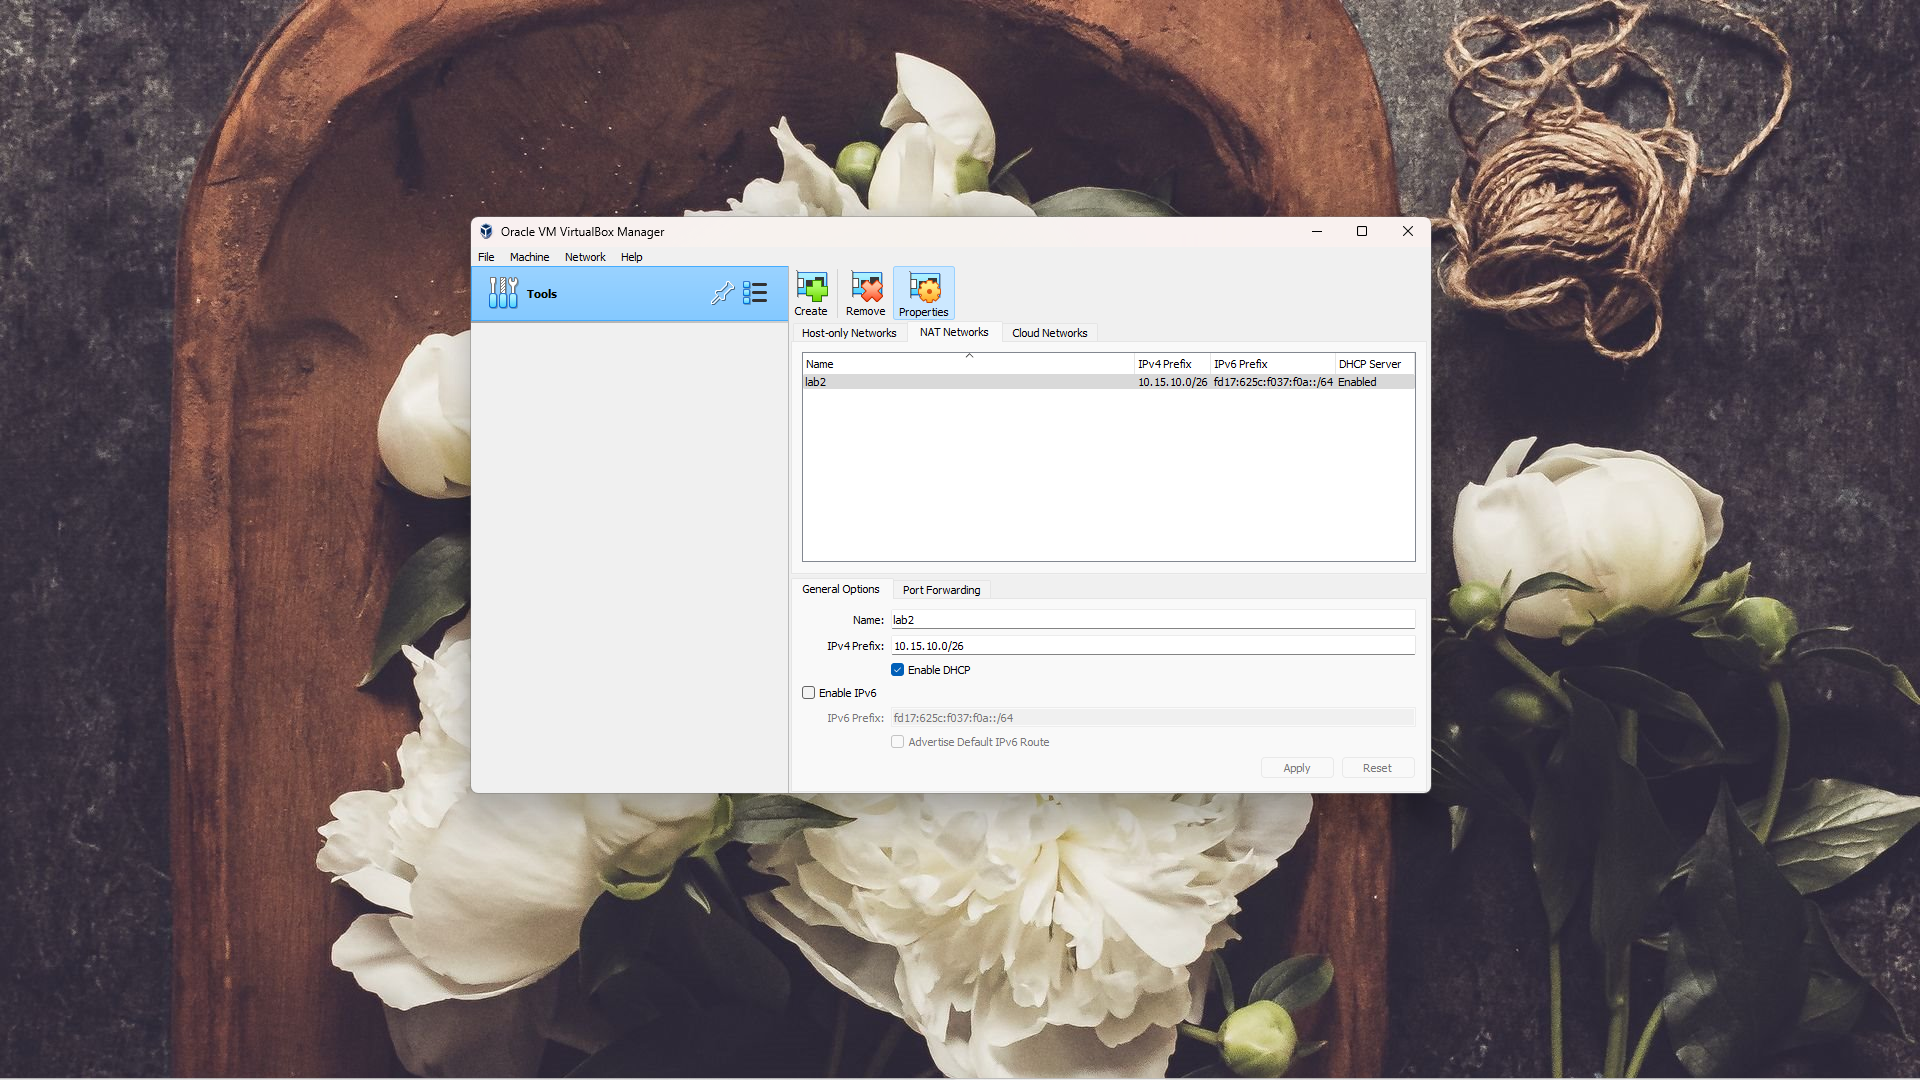
\includegraphics[width=0.85\textwidth]{02_00 (1)}
    \caption{lab2 - настроенная для работы с виртуальными машинами сеть}
    \label{img:0001}
  \end{figure}

  Для осуществления \textit{DHCP} спуффинга создадим 2 виртуальные машины - атакуемого и атакующего.
  Воспользуемся заранее подготовленным образом системы, импортируем его:

  \begin{figure}[H]
    \centering
    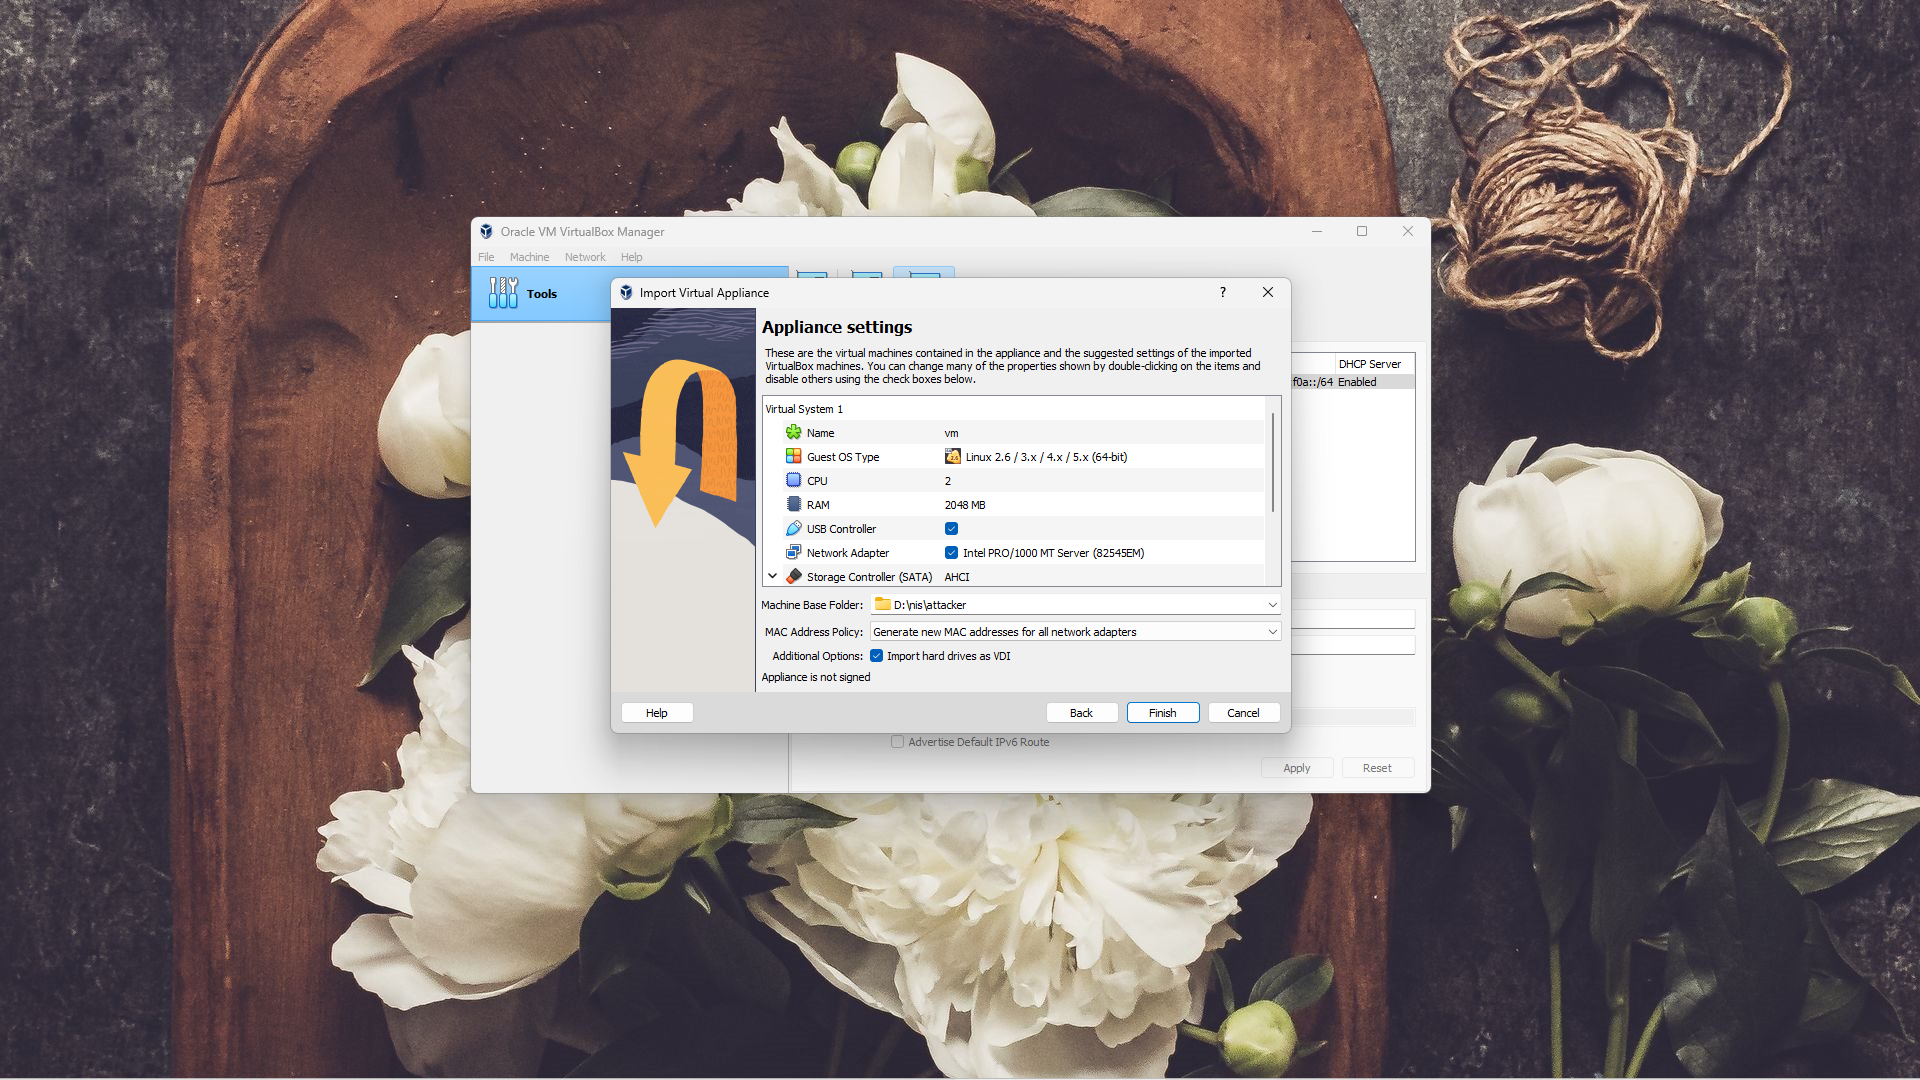
\includegraphics[width=0.85\textwidth]{02_00 (2)}
    \caption{Открываем мастер импорта}
    \label{img:0002}
  \end{figure}

  \begin{figure}[H]
    \centering
    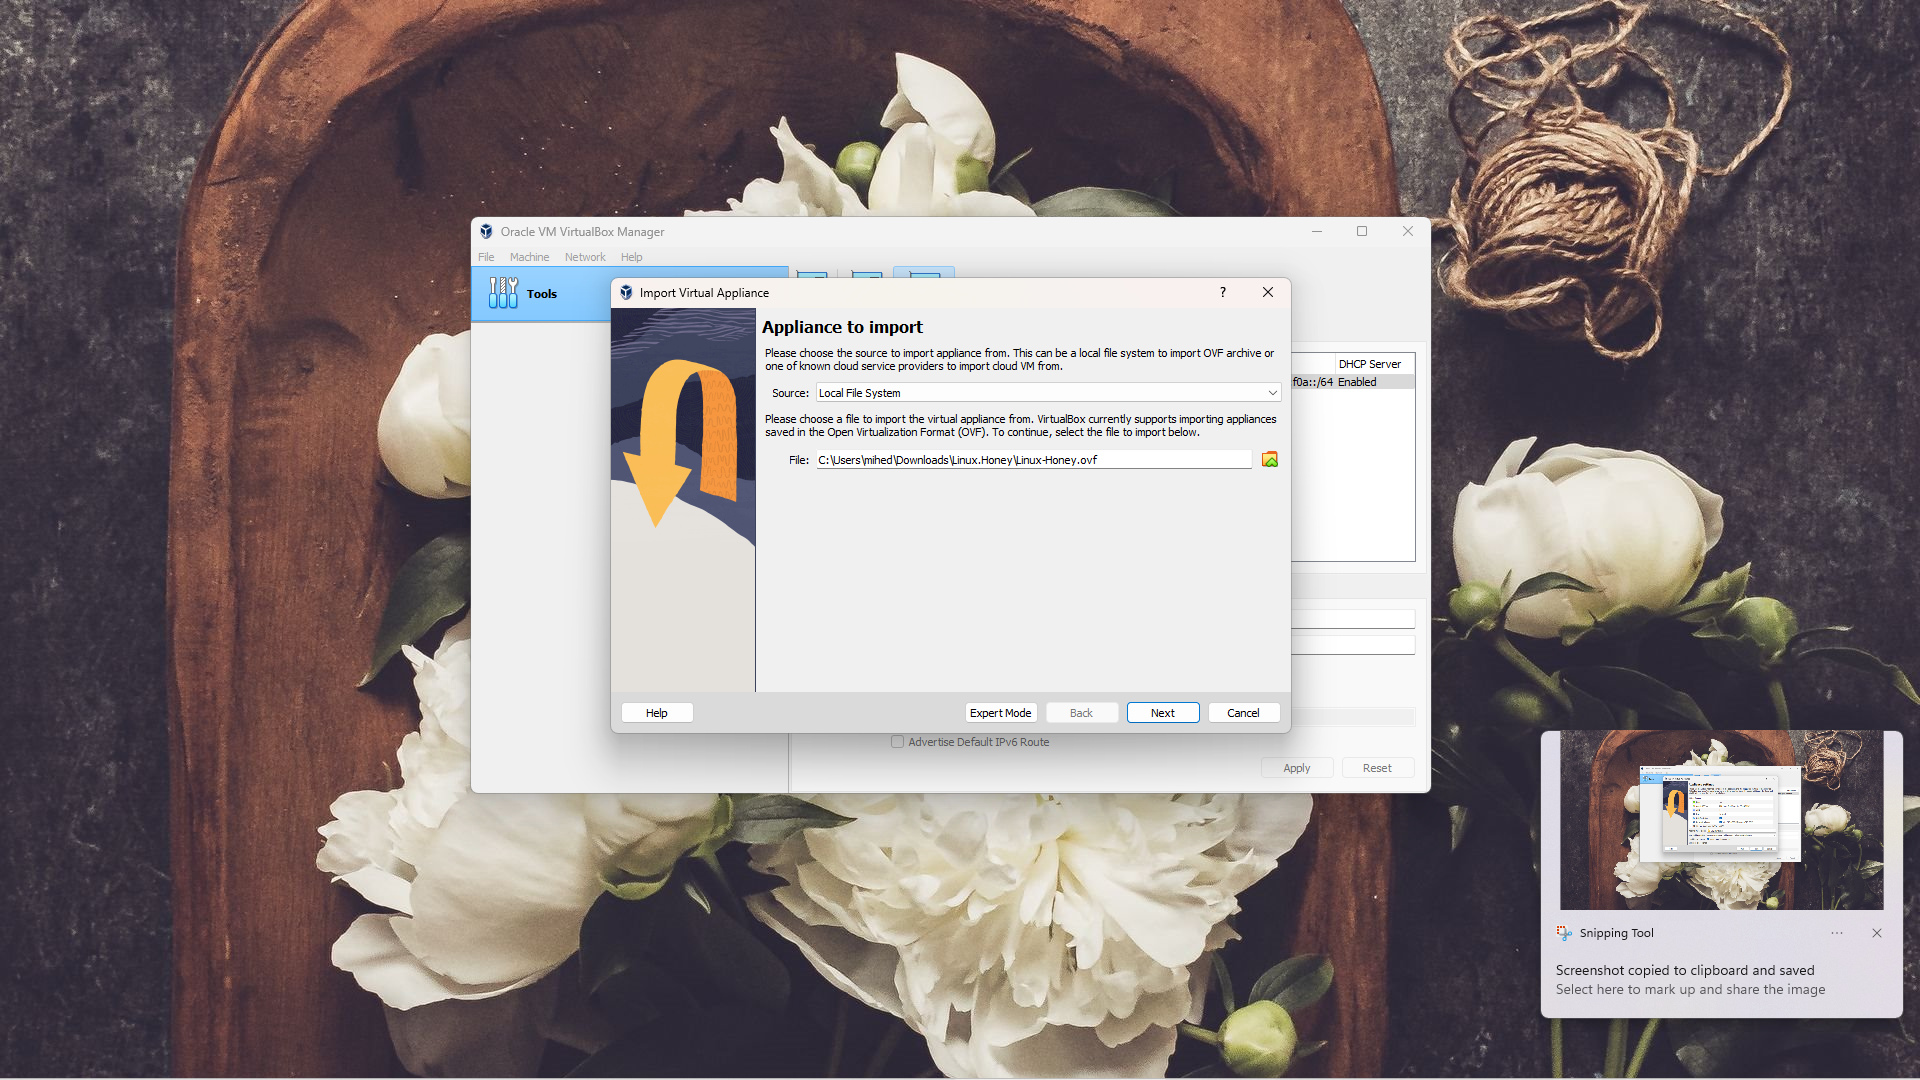
\includegraphics[width=0.85\textwidth]{02_00 (3)}
    \caption{Указываем путь до образа с системой}
    \label{img:0003}
  \end{figure}

  После завершения импорта появилась новая виртуальная машина - настроим ее: укажем новое имя и 
  подключим к ранее созданной сети:

  \begin{figure}[H]
    \centering
    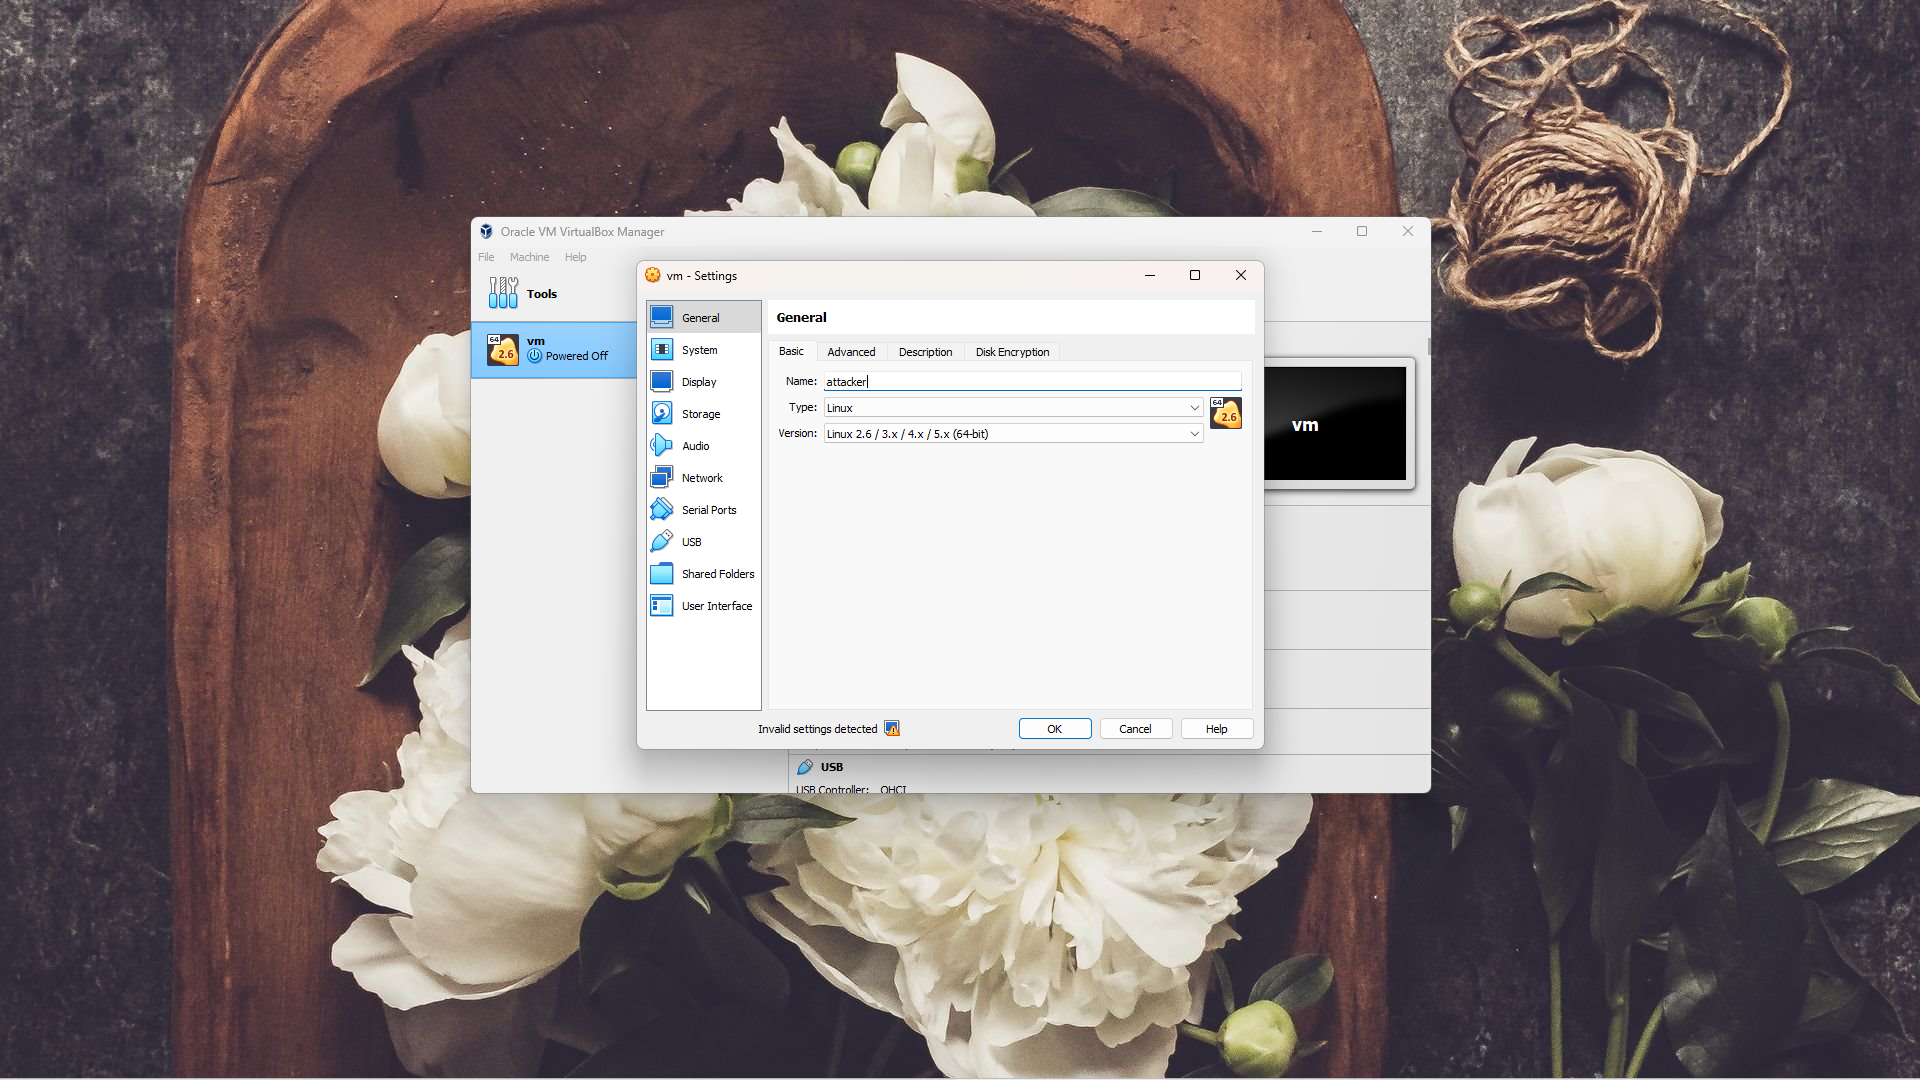
\includegraphics[width=0.85\textwidth]{02_00 (4)}
    \caption{Указываем новое имя для ВМ - attacker}
    \label{img:0004}
  \end{figure}

  \begin{figure}[H]
    \centering
    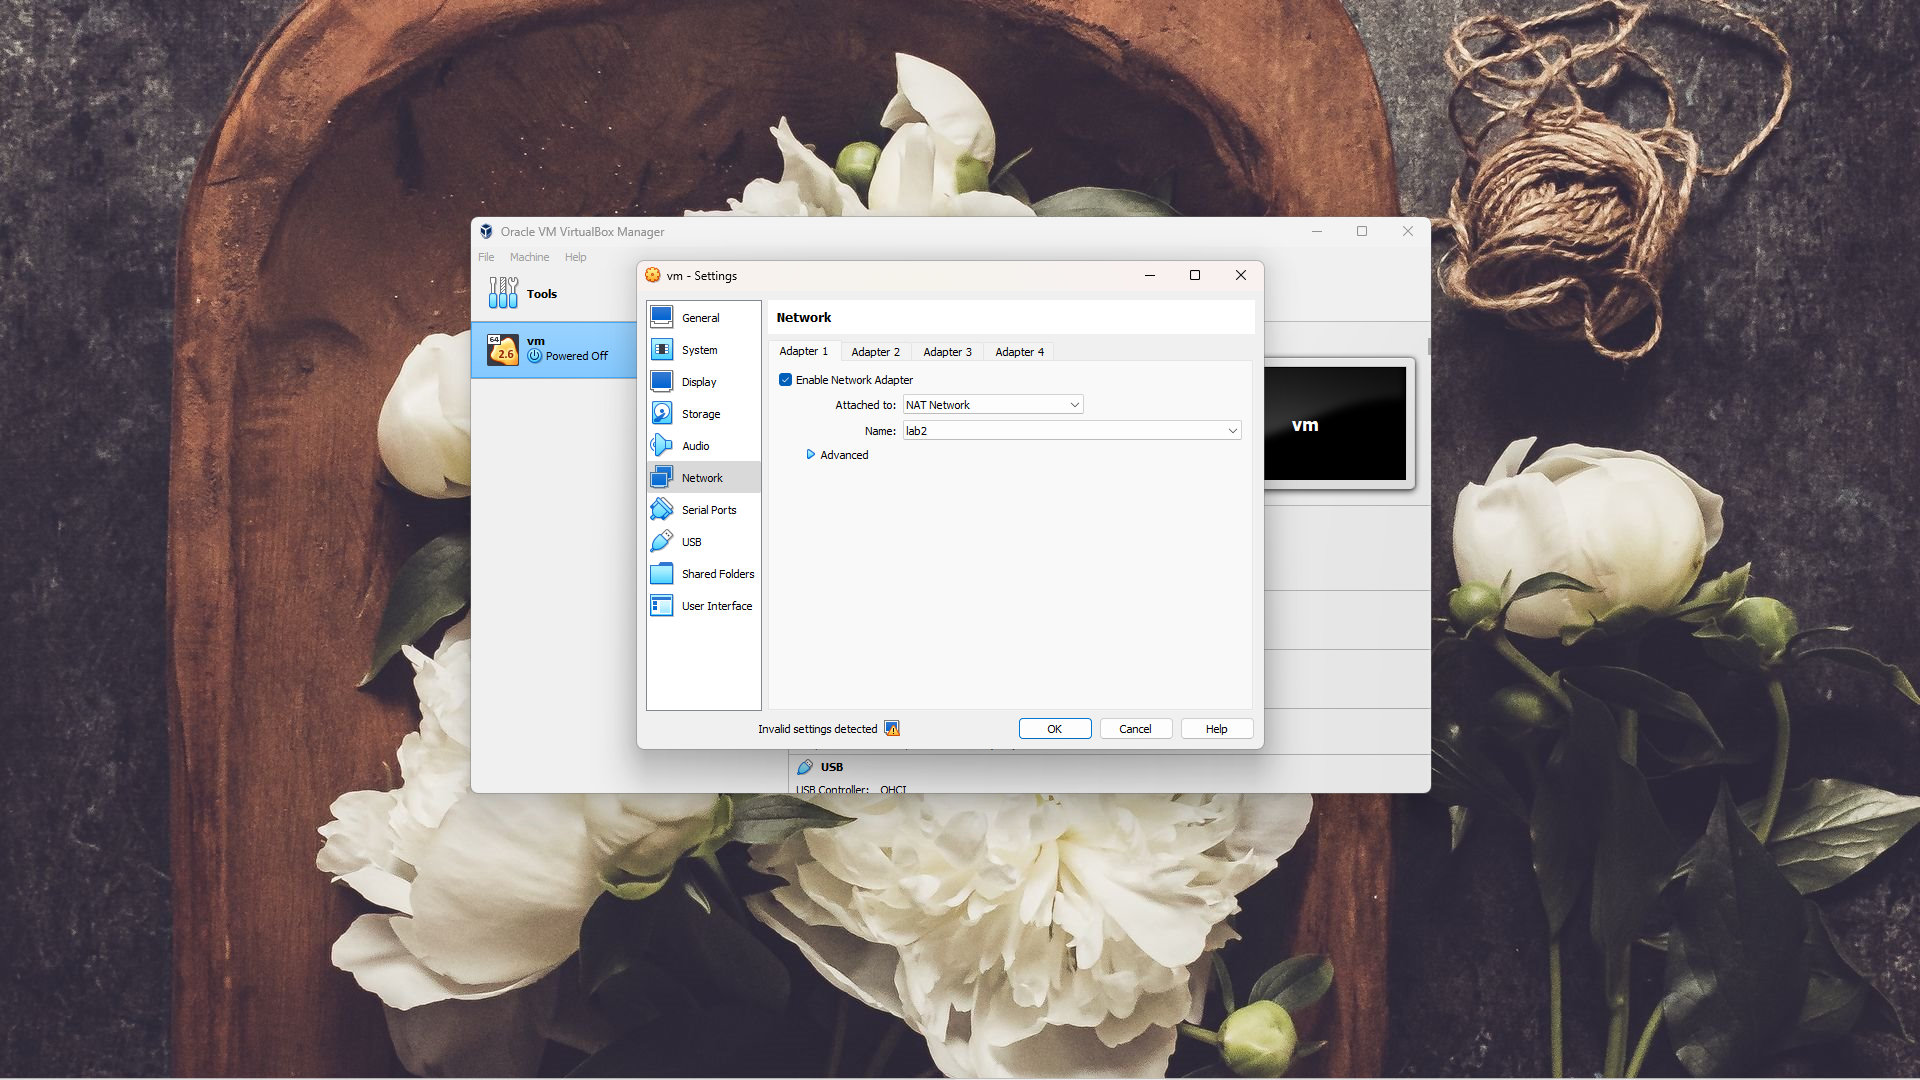
\includegraphics[width=0.85\textwidth]{02_00 (5)}
    \caption{Настраиваем сеть для подключения - lab2}
    \label{img:0005}
  \end{figure}

  Атакуюемую машину создадим точно такую же - при помощь клонирования уже созданного образа:
  
  \begin{figure}[H]
    \centering
    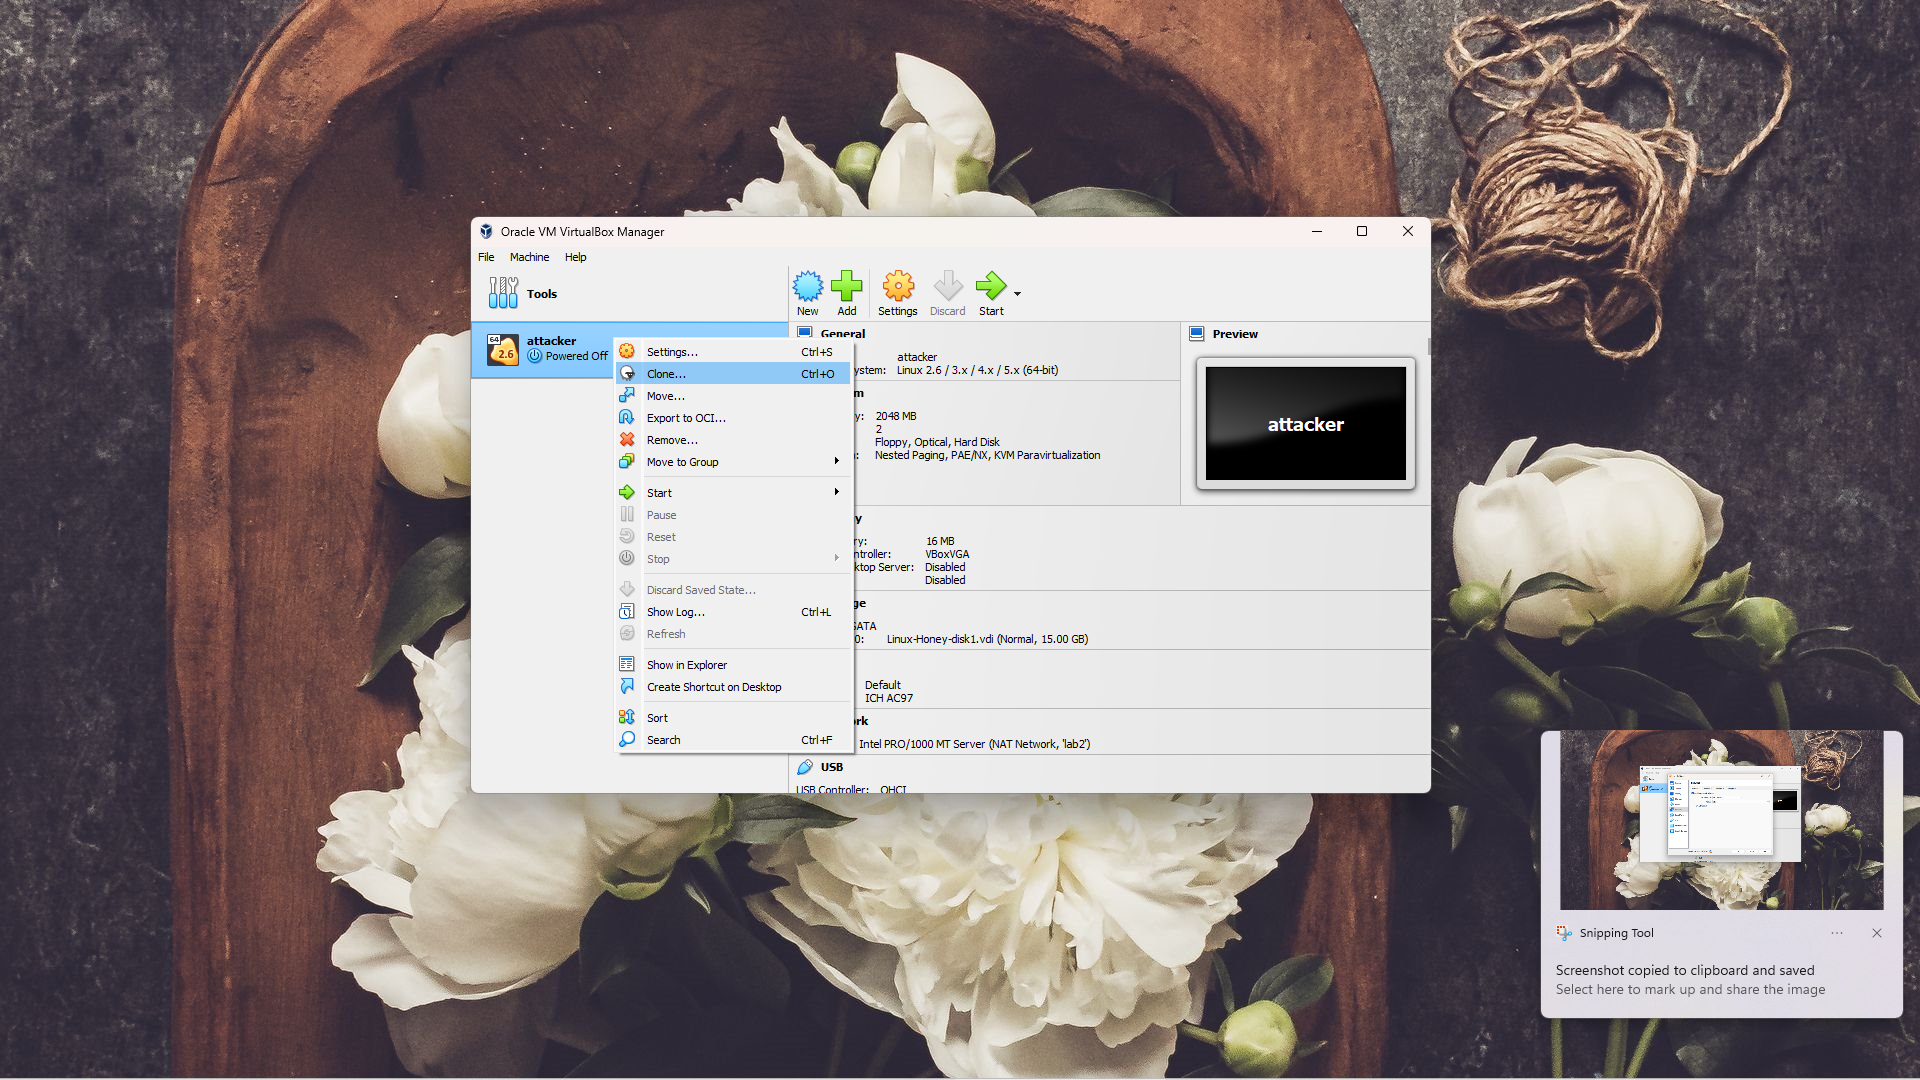
\includegraphics[width=0.85\textwidth]{02_00 (6)}
    \caption{Запускаем процесс клонирования ВМ}
    \label{img:0006}
  \end{figure}

  \begin{figure}[H]
    \centering
    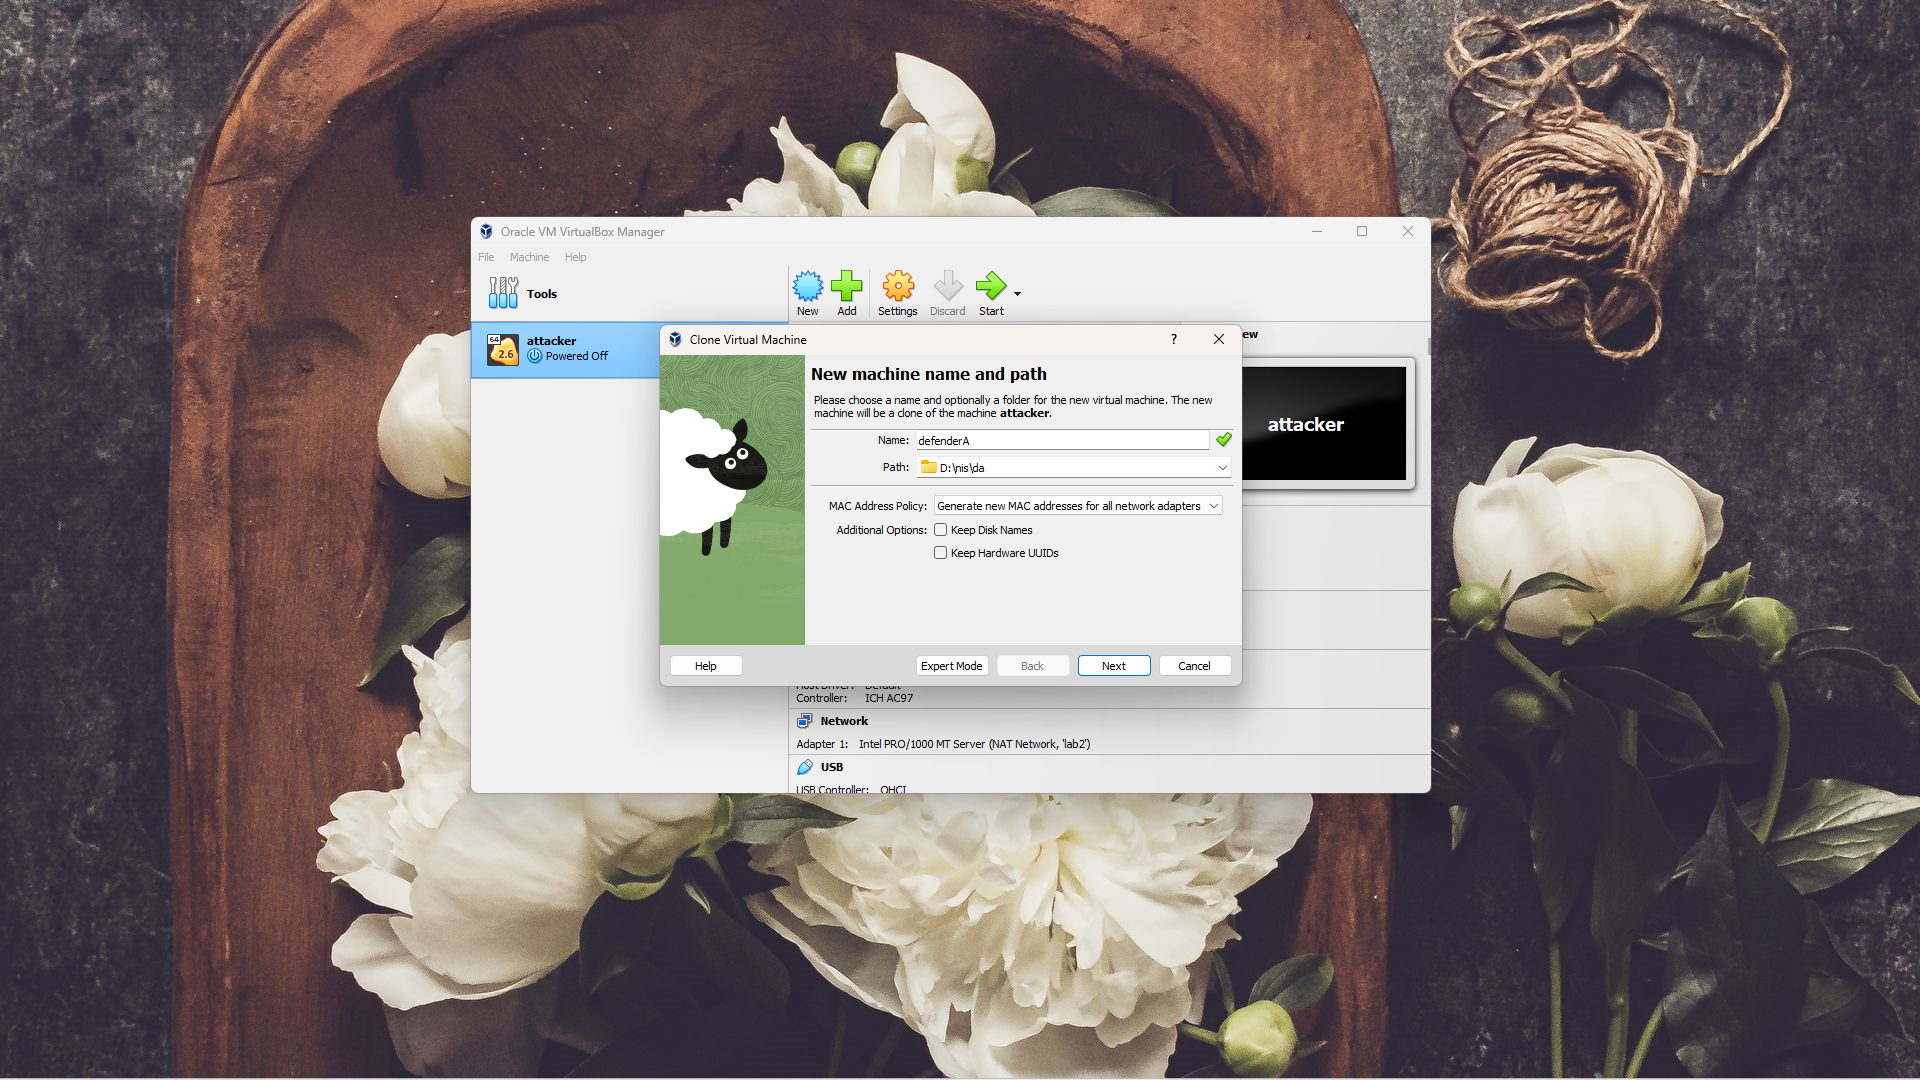
\includegraphics[width=0.85\textwidth]{02_00 (7)}
    \caption{Указываем имя и расположение новой ВМ}
    \label{img:0007}
  \end{figure}

  В итоге получилось две виртуальные машины (\textit{Attacker} и \textit{DefenderA}), подключенные к 
  одной сети с NAT:

  \begin{figure}[H]
    \centering
    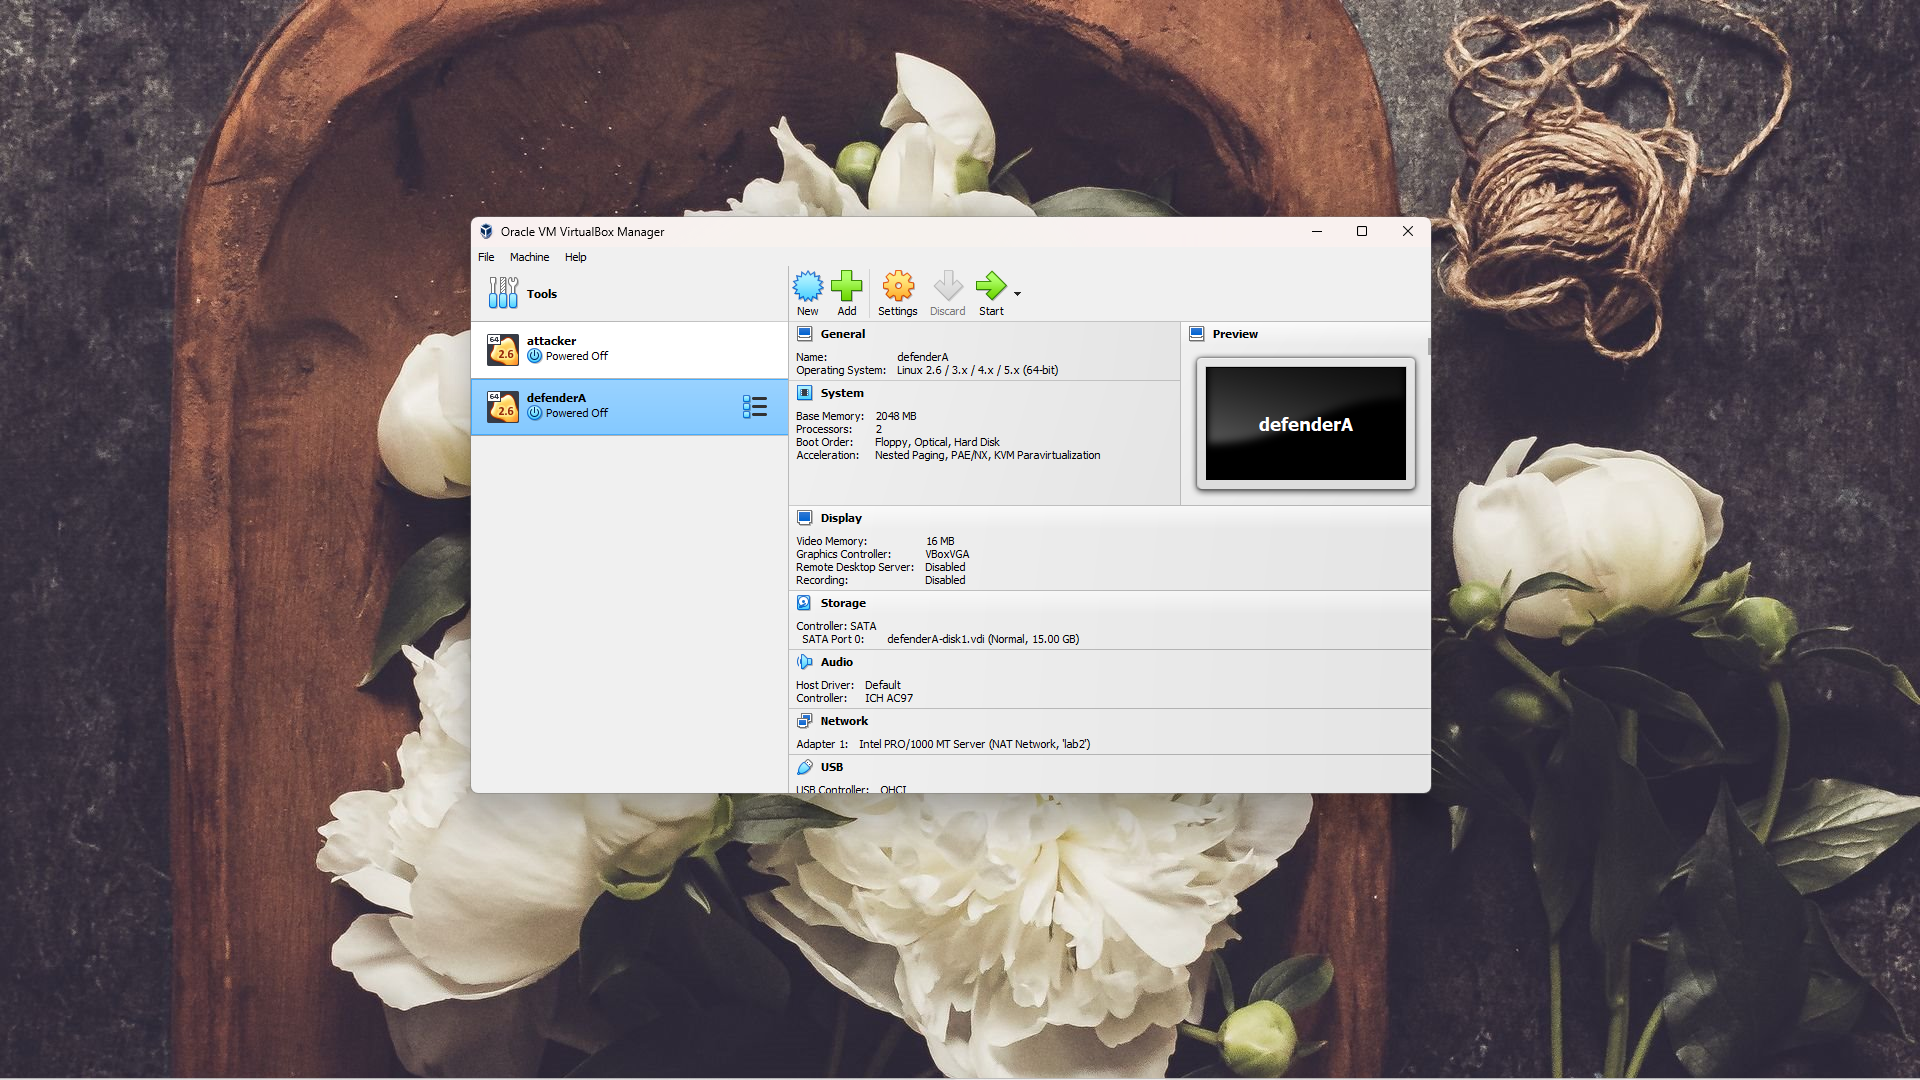
\includegraphics[width=0.85\textwidth]{02_00 (8)}
    \caption{Полученные виртуальные машины}
    \label{img:0008}
  \end{figure}

  \subsubsection{Настройка атакующей машины}

  Запустим и настроим атакующую машины. Для осуществления \textit{DHCP} спуффинга необходимо
  установить пакет \textit{ettercap-graphical}, а для анализа трафика - \textit{Wireshark}.

  Для начала обновим все установленные в системе пакеты и их источники:

  \begin{figure}[H]
    \centering
    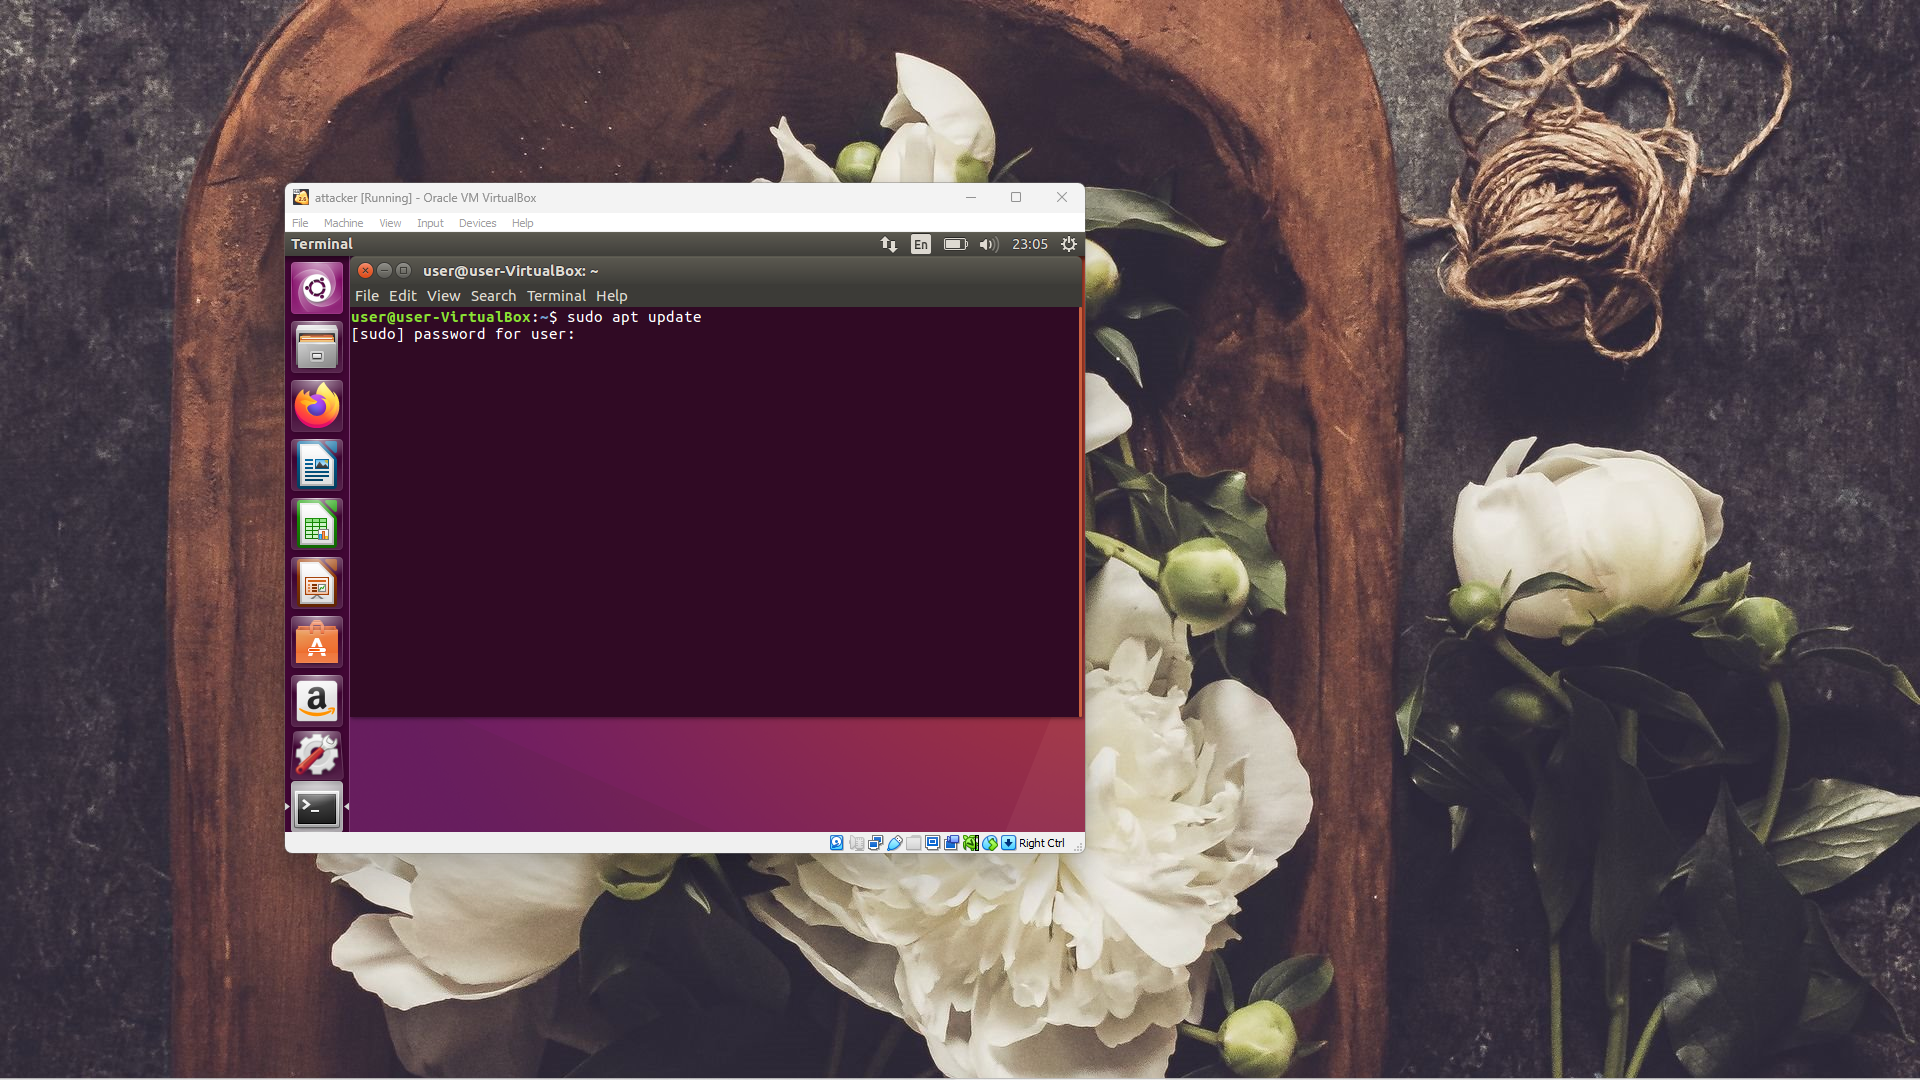
\includegraphics[width=0.85\textwidth]{02_00 (10)}
    \caption{sudo apt update - обновление списка репозиториев}
    \label{img:0009}
  \end{figure}

  \begin{figure}[H]
    \centering
    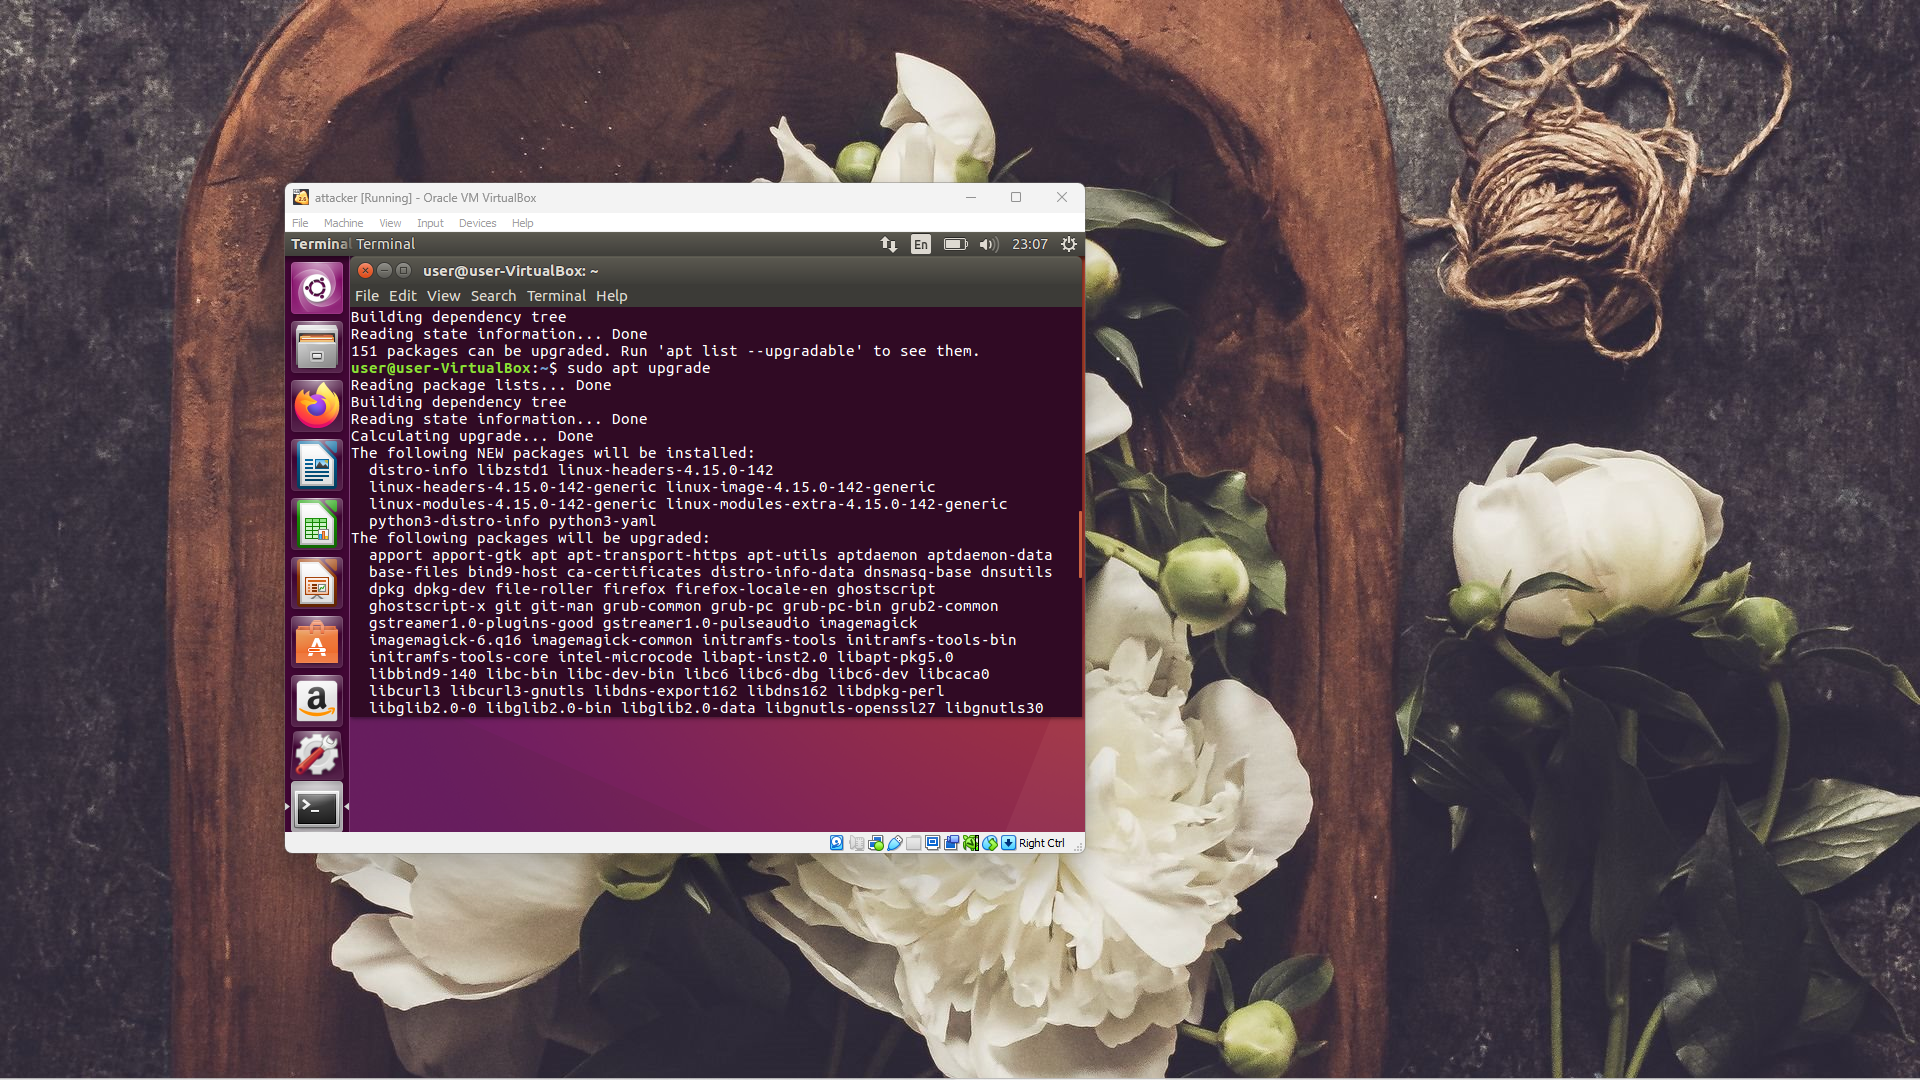
\includegraphics[width=0.85\textwidth]{02_00 (12)}
    \caption{sudo apt upgrade - обновление установленных пакетов}
    \label{img:0010}
  \end{figure}

  Теперь, когда система обновлена, установим необходимые пакеты:

  \begin{figure}[H]
    \centering
    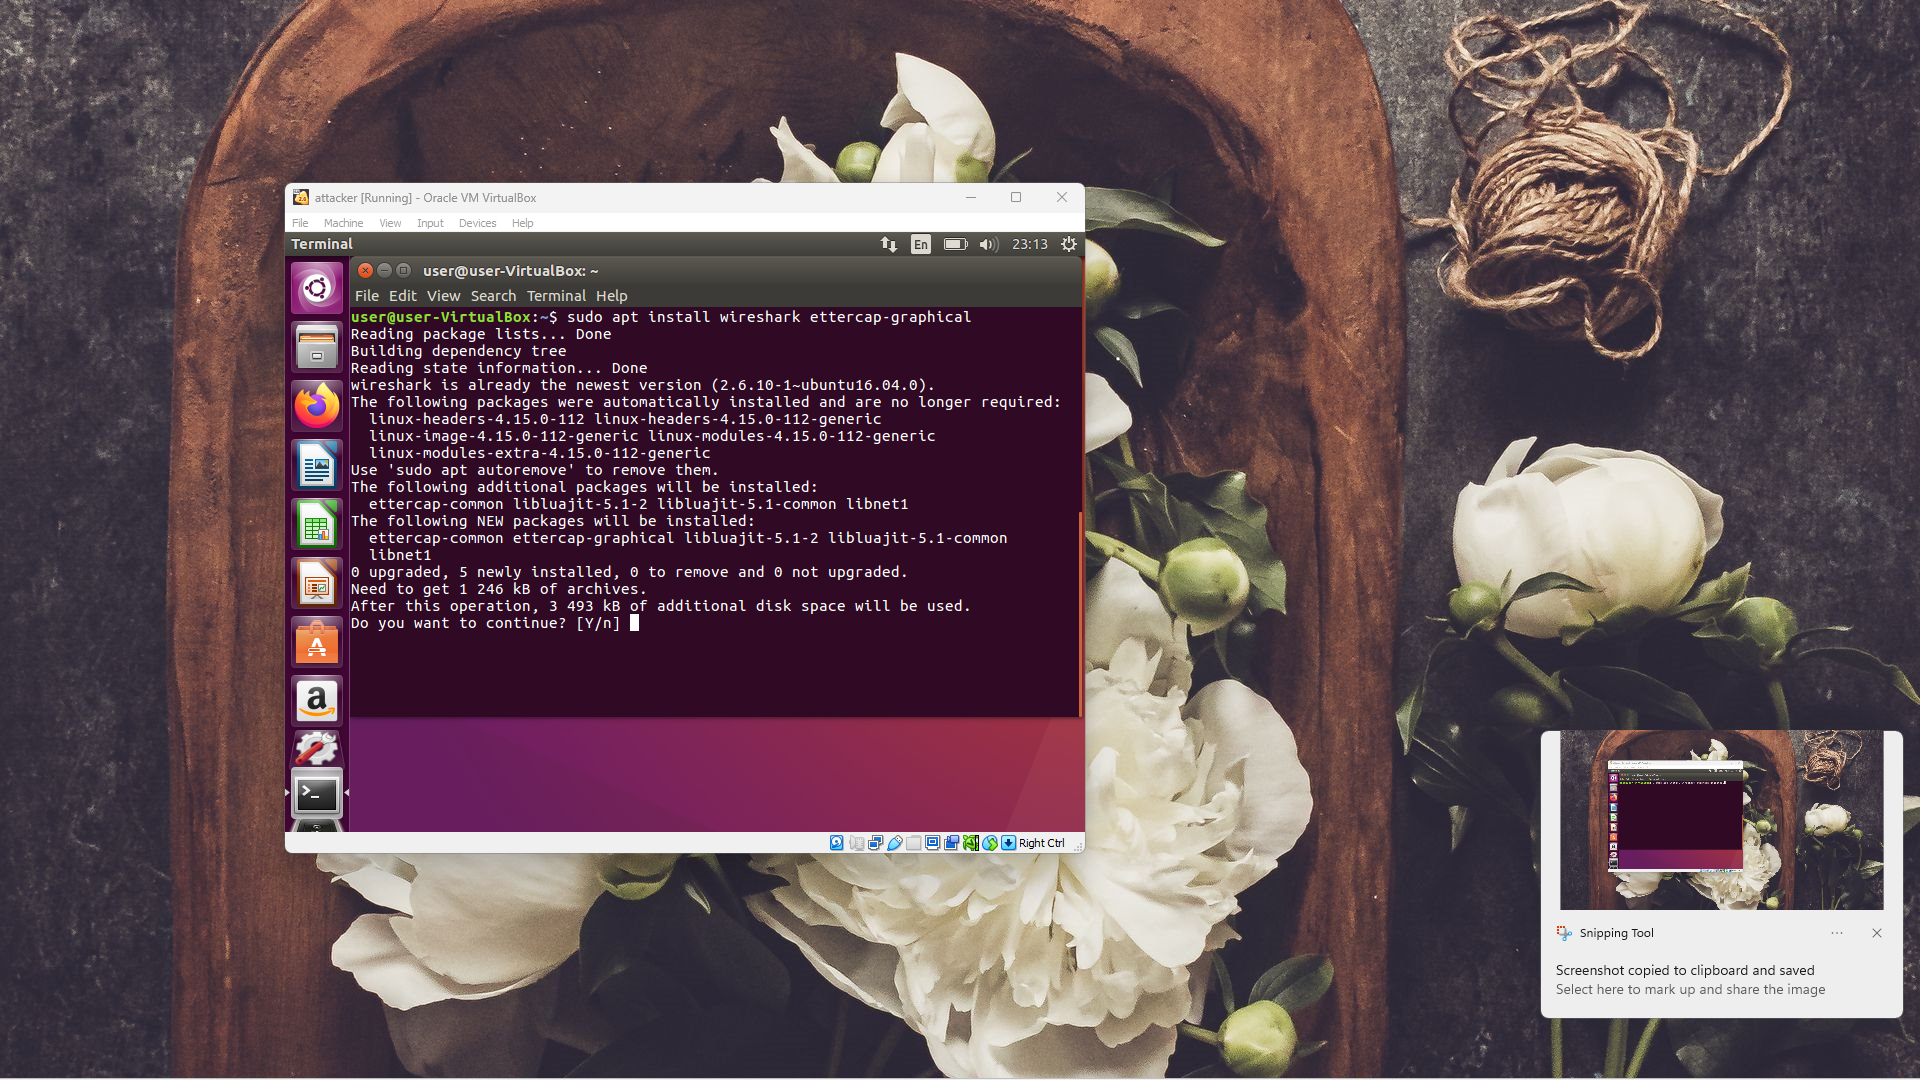
\includegraphics[width=0.85\textwidth]{02_00 (14)}
    \caption{sudo apt install wireshark ettercap-graphical}
    \label{img:0011}
  \end{figure}

  \subsubsection{Проверка параметров и работоспособности сети}

  Узнаем \textit{MAC} и \textit{IPv4} адреса атакующей и атакуемой машины, для этого воспользуемя 
  встроенной утилитой \textit{ip}:

  \begin{figure}[H]
    \centering
    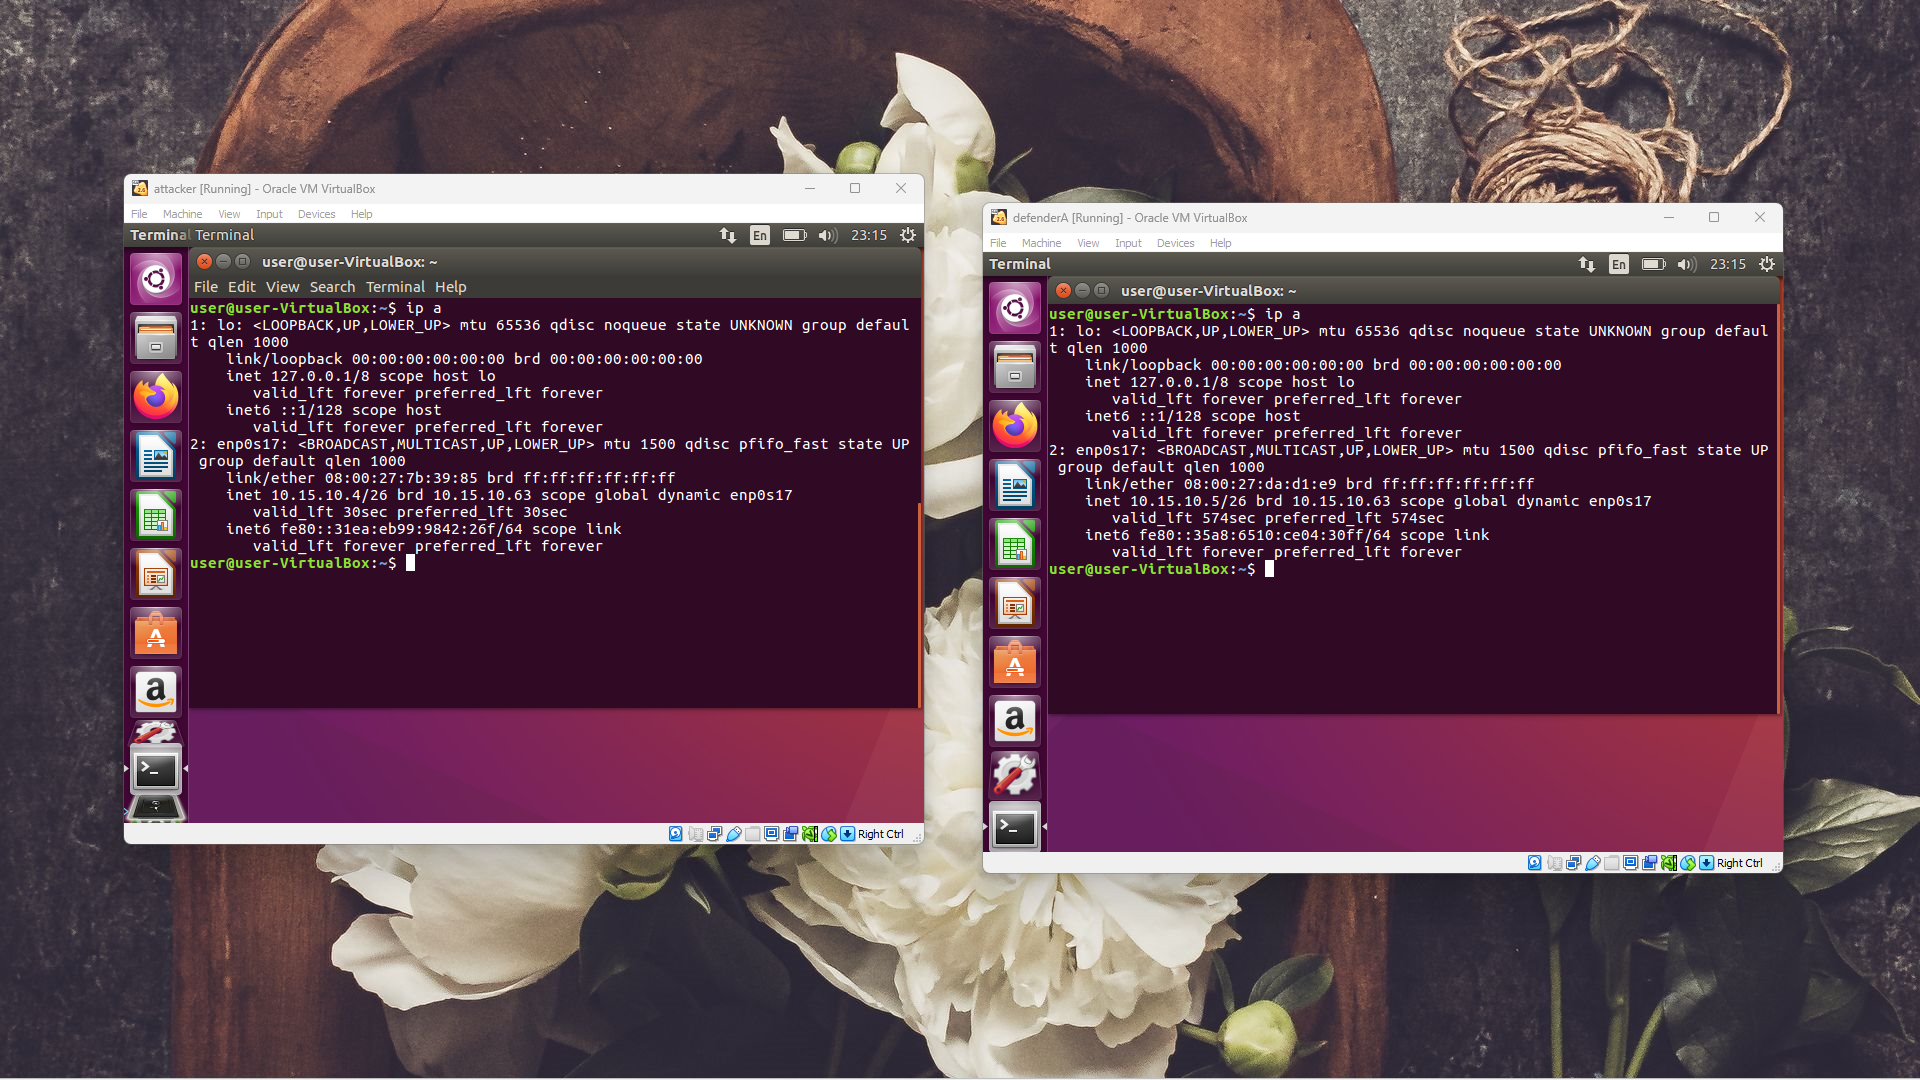
\includegraphics[width=0.85\textwidth]{02_00 (15)}
    \caption{Получение информации о сетевых интерфейсах машин}
    \label{img:0012}
  \end{figure}

  Рассмотрим полученную информацию:

  \begin{table}[H]
    \centering
    \begin{tabular}{| c | c | c | c | c |}
      \hline
      Имя ВМ & Статут & Сетевой интерфейс & MAC-адрес & IPv4-адрес \\
      \hline
      Attacker & Атакующий & enp0s17 & 08:00:27:7b:39:85 & 10.15.10.4 \\
      \hline
      DefenderA & Атакуемый & enp0s17 & 08:00:27:da:d1:e9 & 10.15.10.5 \\
      \hline
    \end{tabular}
    \caption{Информация о сетвых параметрах машин}
  \end{table}

  Проверим, что виртуальные машины могут связываться друг с другом - пропингуем атакующего с атакуемой,
  а атакуюему с атакующей машины при помощи \textit{ping}:

  \begin{figure}[H]
    \centering
    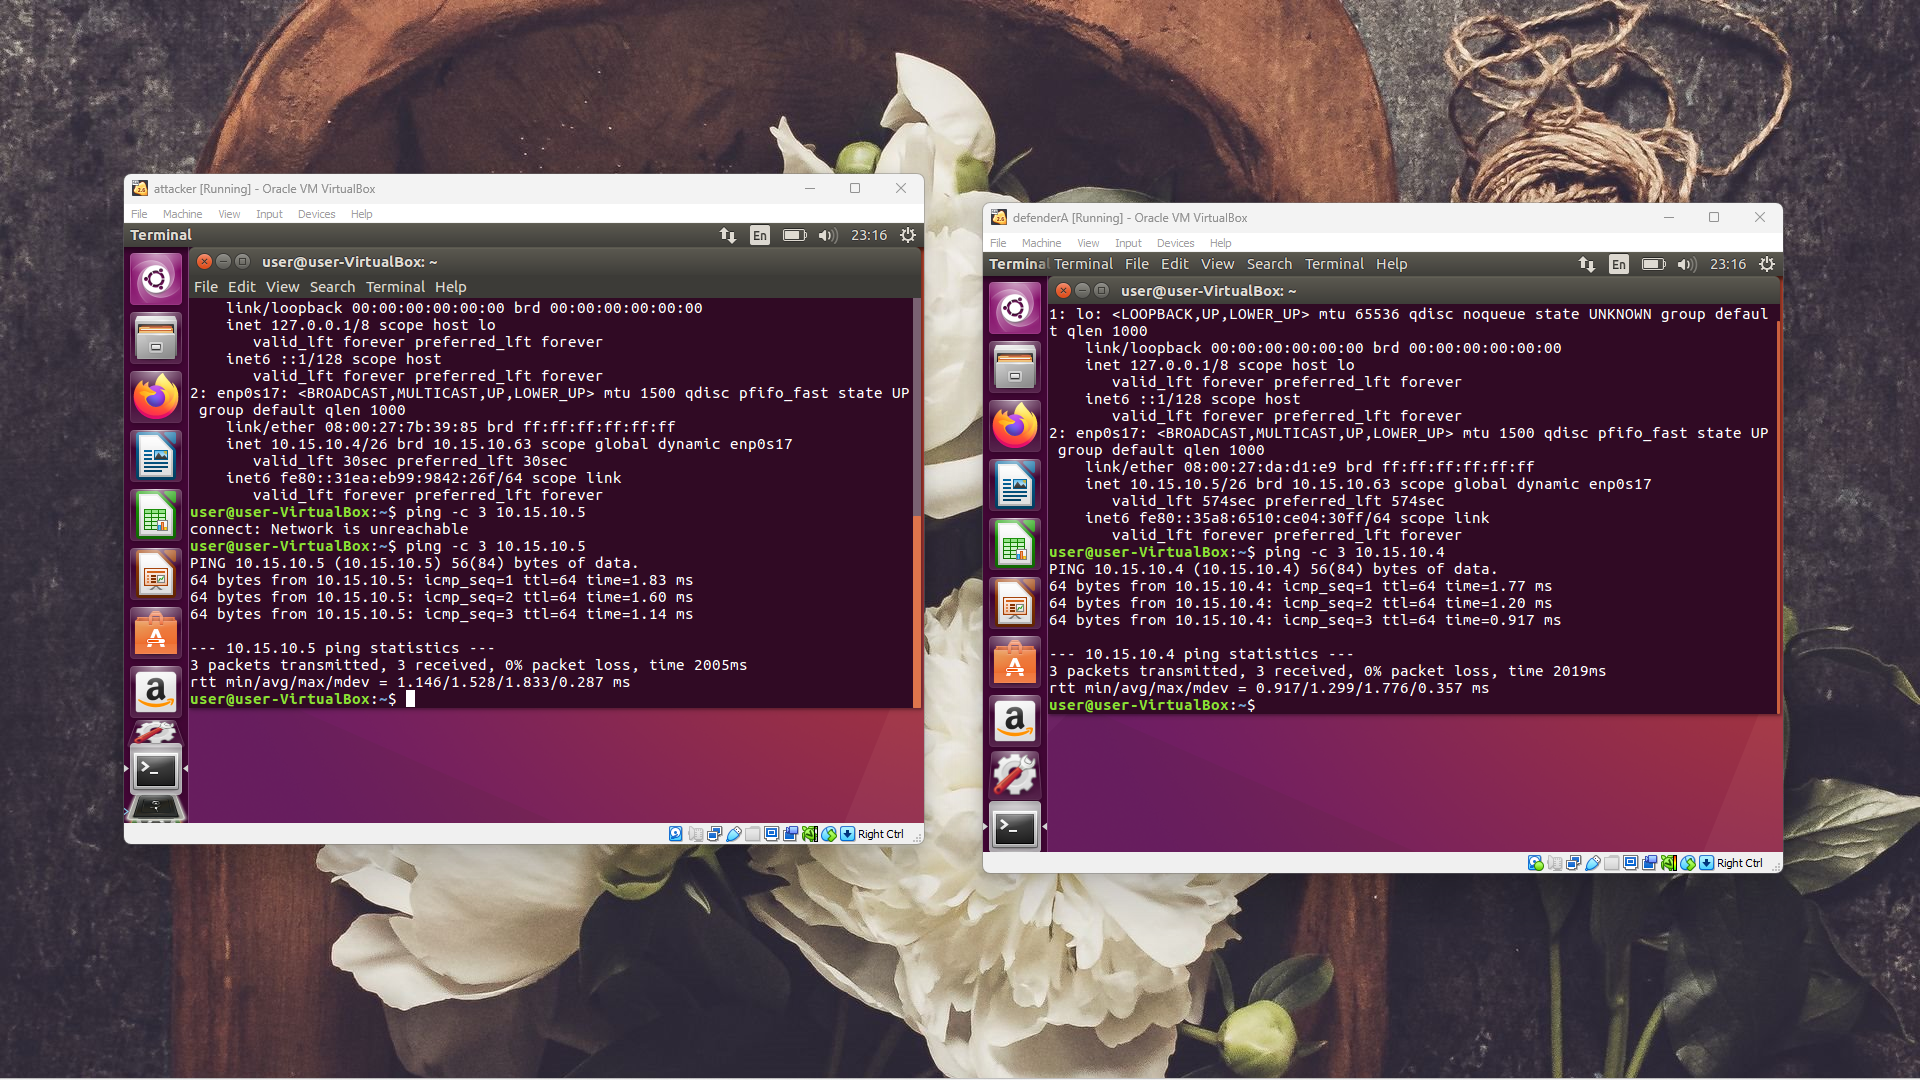
\includegraphics[width=0.85\textwidth]{02_00 (16)}
    \caption{Проверка доступности}
    \label{img:0013}
  \end{figure}

  \subsubsection{Подготовка к спуффингу}

  Чтобы понять, что происходит во время спуффинга, запустим сниффер - \textit{Wireshark}:

  \begin{figure}[H]
    \centering
    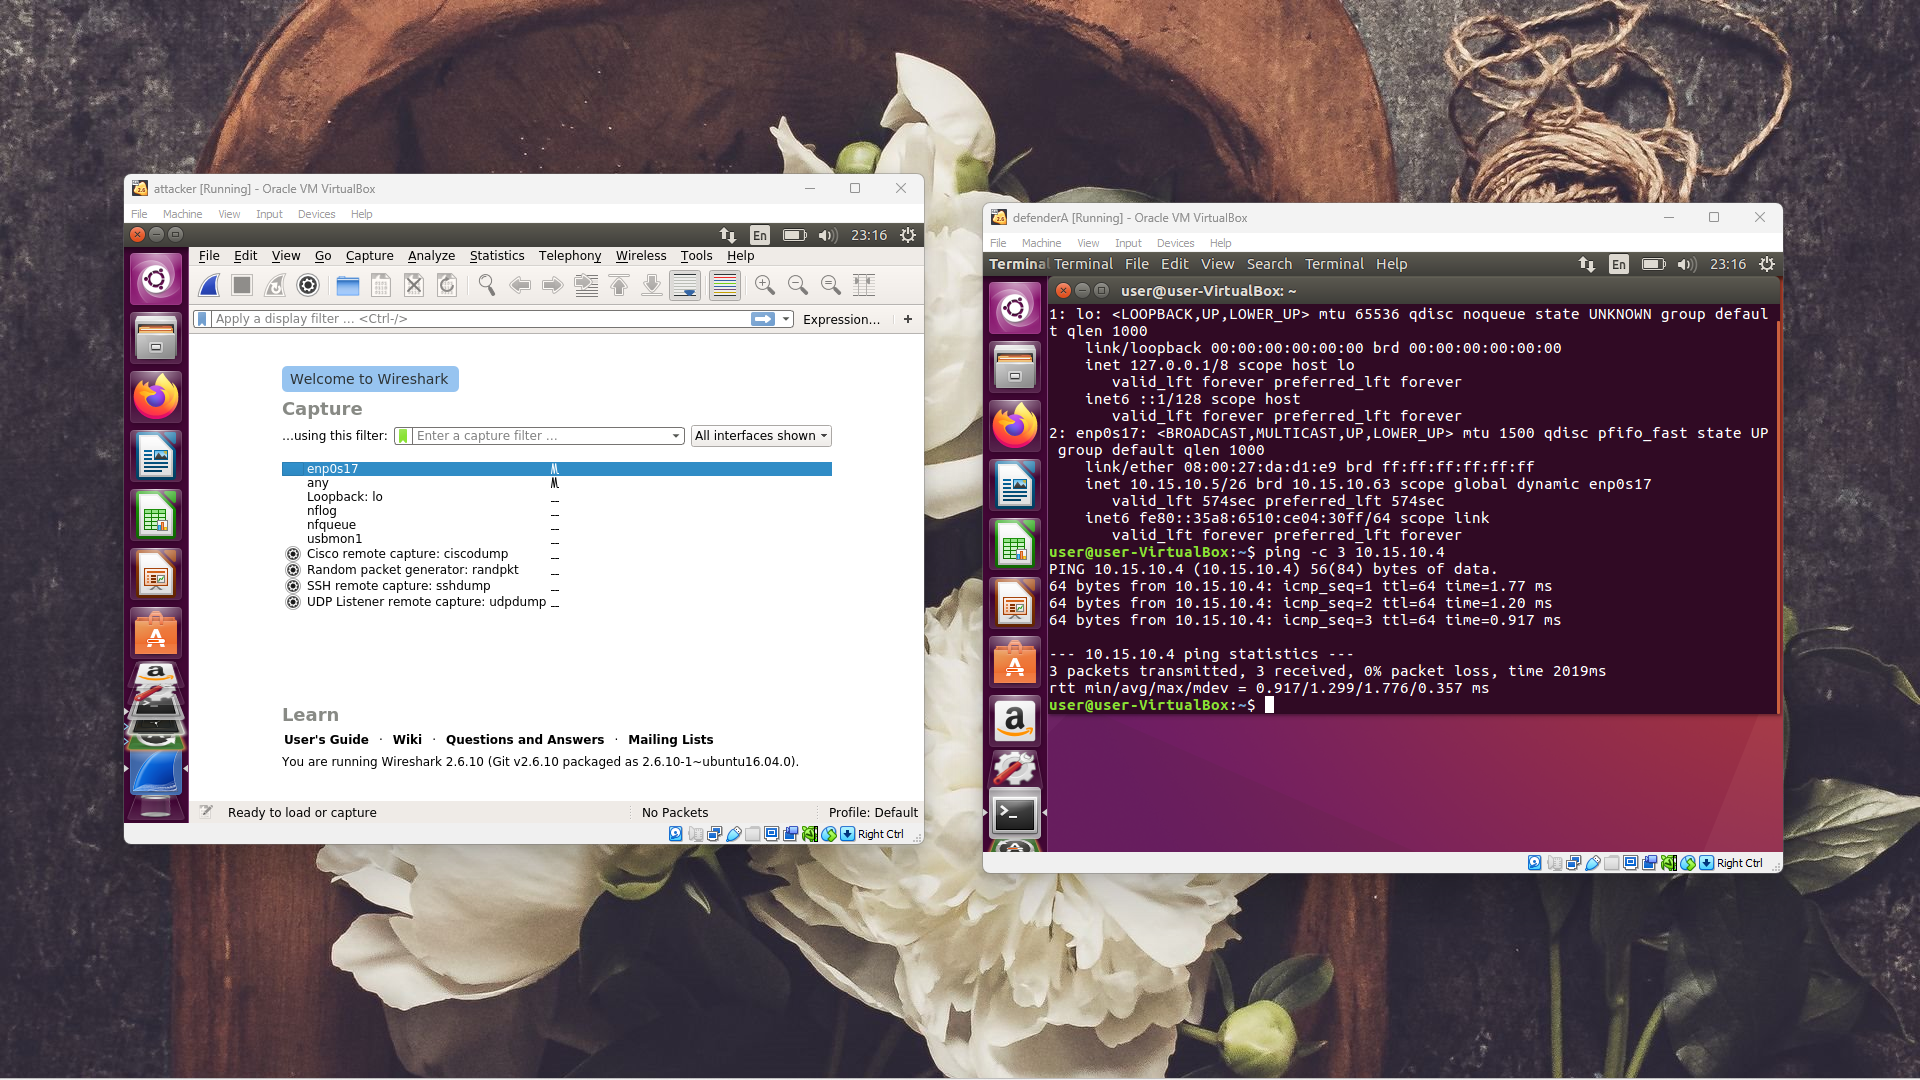
\includegraphics[width=0.85\textwidth]{02_00 (17)}
    \caption{Запускаем wireshark и выбираем нужный интерфейс}
    \label{img:0014}
  \end{figure}

  \begin{figure}[H]
    \centering
    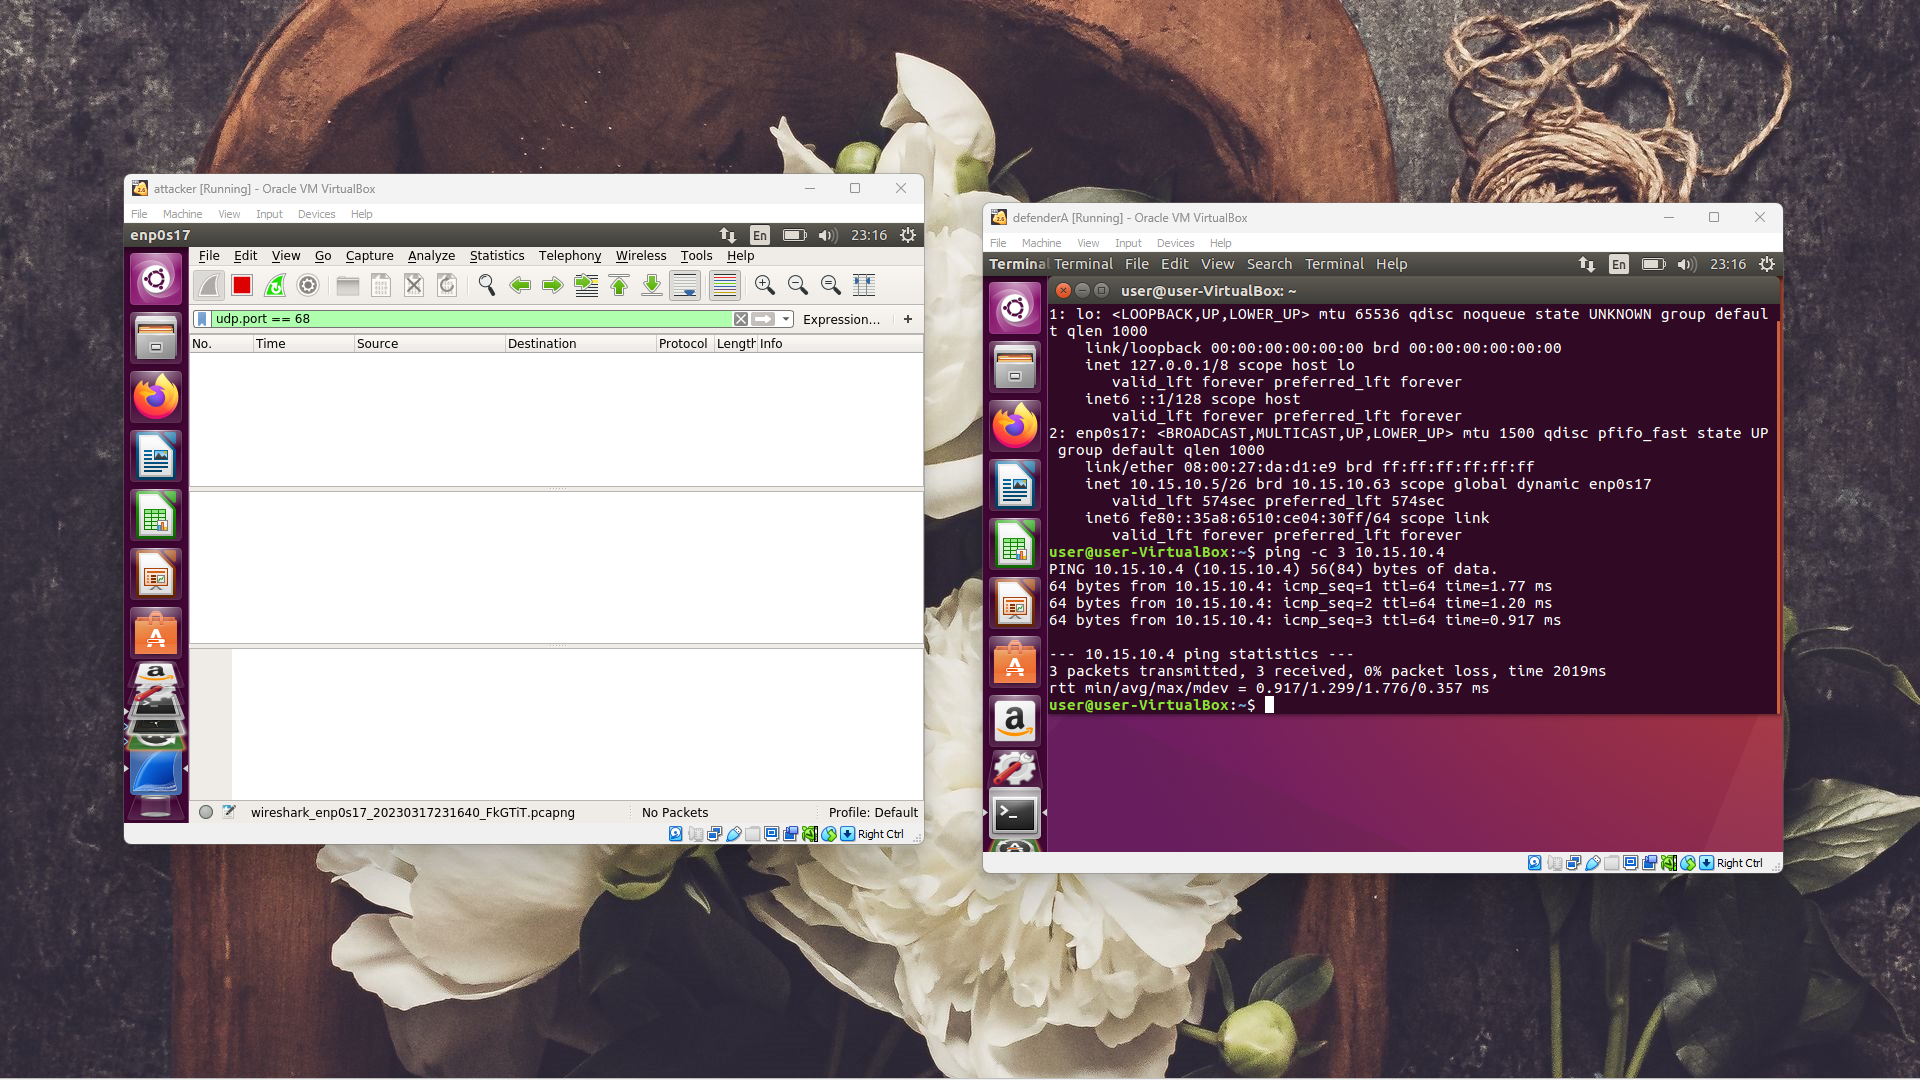
\includegraphics[width=0.85\textwidth]{02_00 (18)}
    \caption{Устанавливаем фильтр на порт, чтобы анализировать только DHCP-пакеты}
    \label{img:0015}
  \end{figure}

  Сбросим \textit{IP} атакуемой машины и запросим для нее новый при помощи \textit{dhclient}:
  
  \begin{figure}[H]
    \centering
    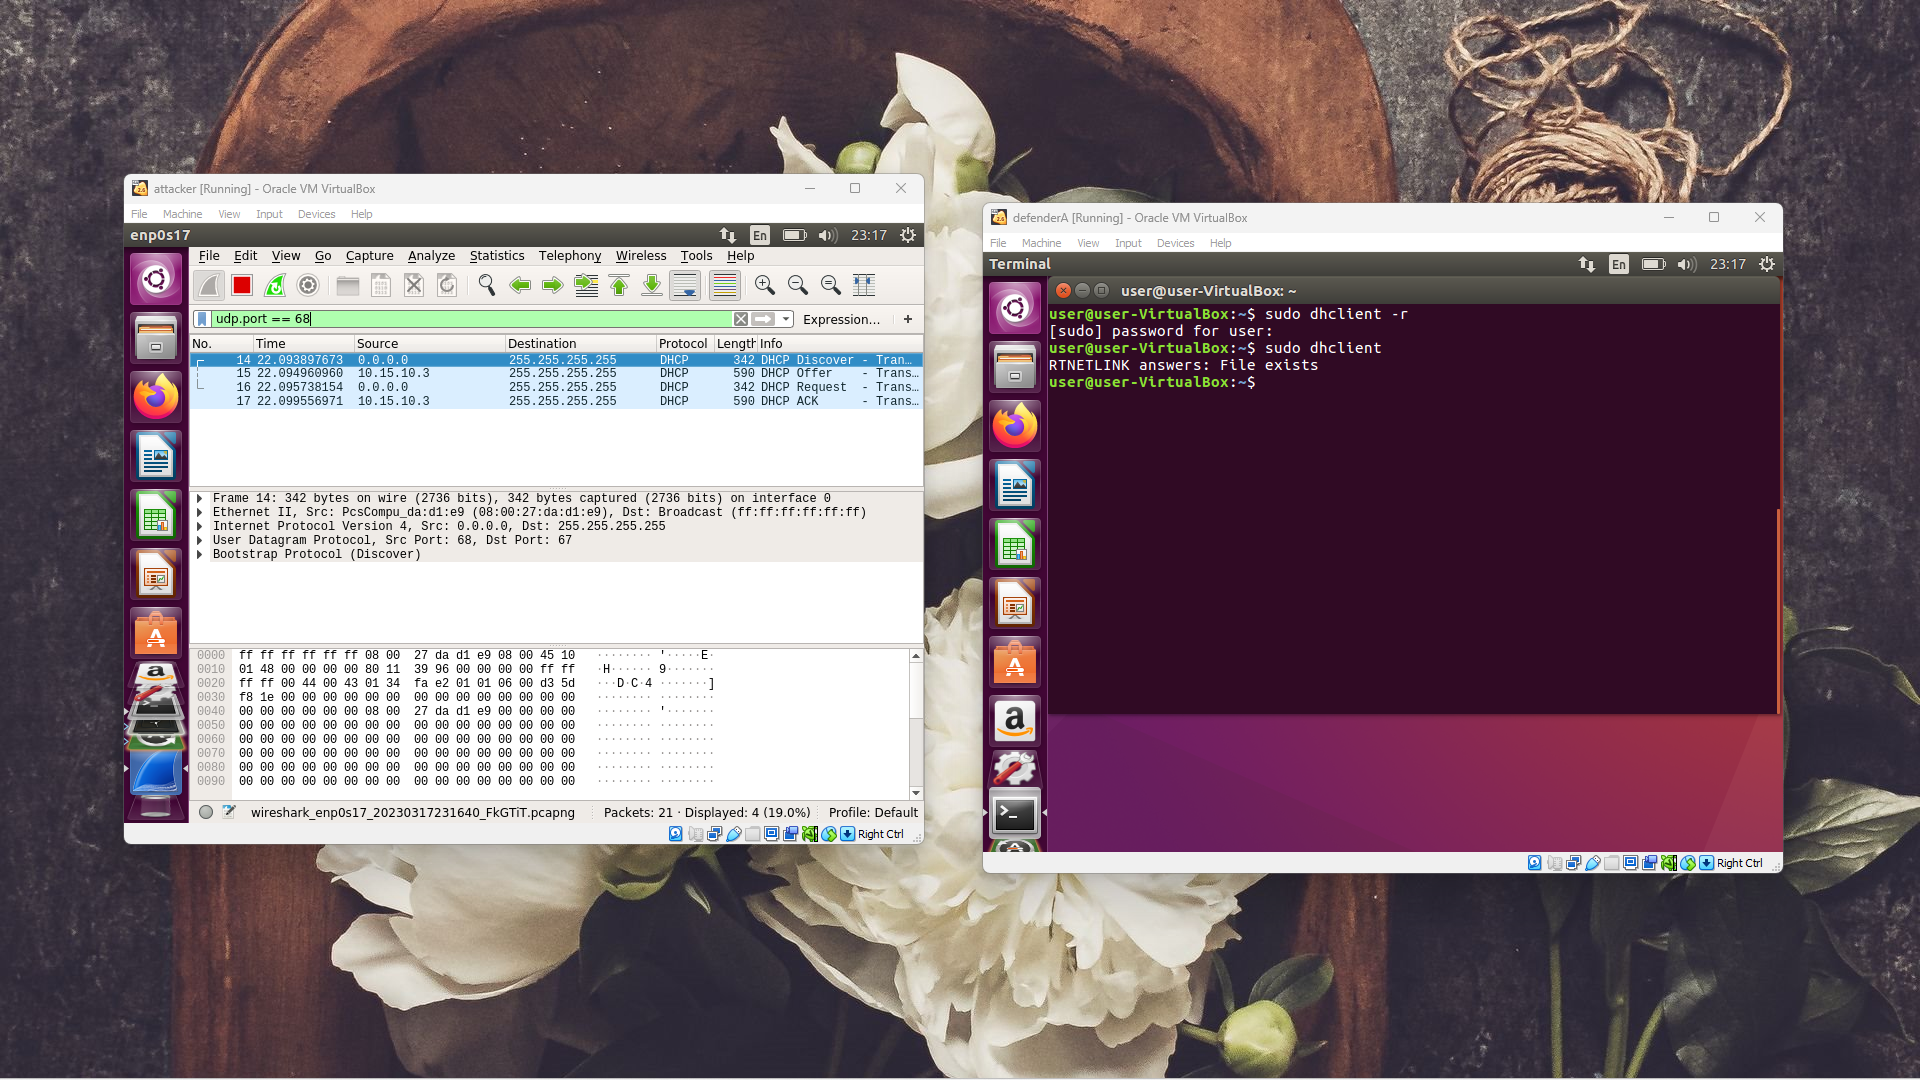
\includegraphics[width=0.85\textwidth]{02_00 (19)}
    \caption{Сброс и запрос нового IP адреса}
    \label{img:0016}
  \end{figure}

  Рассмотрим перехваченные пакеты. Первым пришел \textit{DHCP Discover} запрос - атакуемая машина,
  оставшись без \textit{IP} адреса после выполнения команды \textit{sudo dhclient -r}, отправила
  широковещательный запрос на поиск \textit{DHCP} сервера для текущей сети. Далее последовал ответ от \textit{DHCP}-сервера,
  расположенного по адресу 10.15.10.3 - \textit{DHCP offer}:

  \begin{figure}[H]
    \centering
    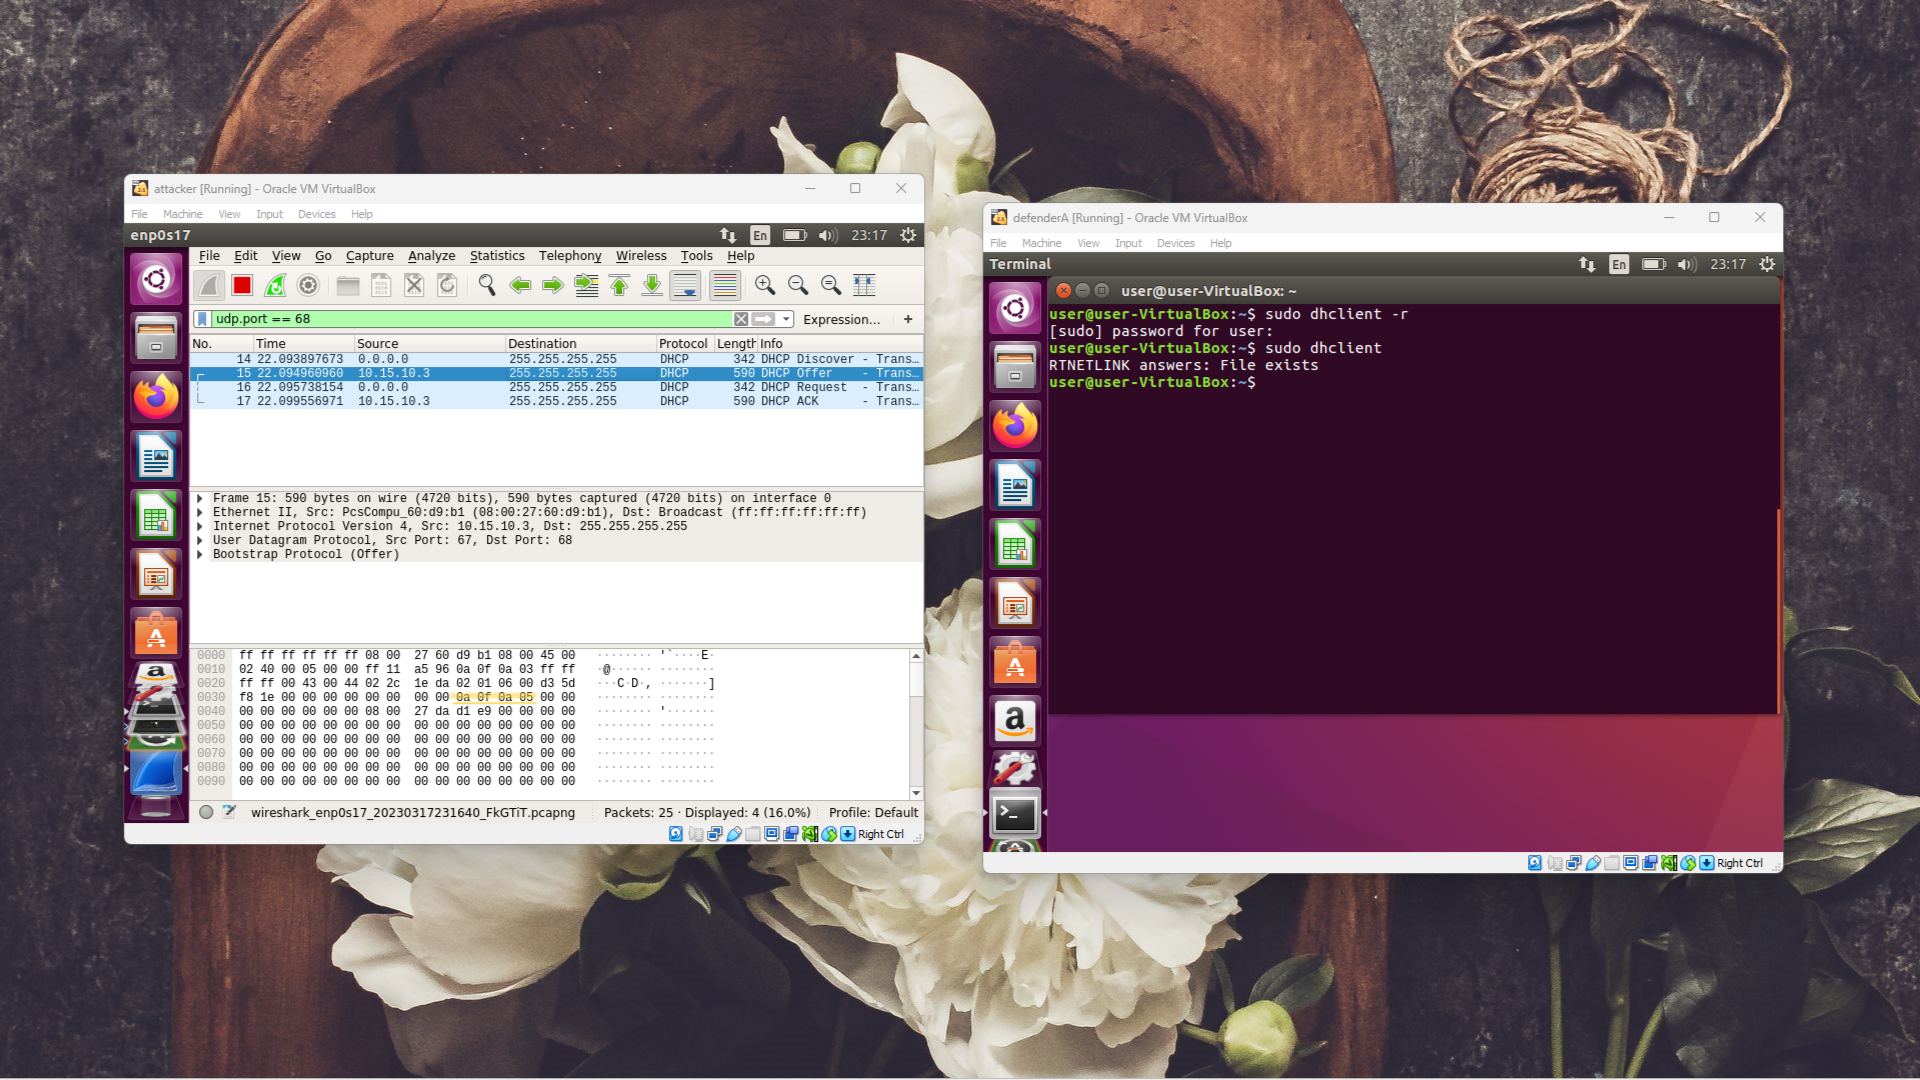
\includegraphics[width=0.85\textwidth]{02_00 (20)}
    \caption{DHCP Offer}
    \label{img:0017}
  \end{figure}

  Внимательно изучим пакет - видно, что нашей машине предложили взять
  адрес 10.15.10.5 (обведено желтым). У атакуемой машины не было ограничений на \textit{IP}
  адрес, поэтому она отправила \textit{DHCP Request} - запрос, чтобы за ней закрепили
  ранее предложенный адрес. Позже последовал положительный \textit{DHCP ACK} ответ.

  Как результат, \textit{ip a} показывает, что текущая машина имеет \textit{IP} адрес
  10.15.10.5:

  \begin{figure}[H]
    \centering
    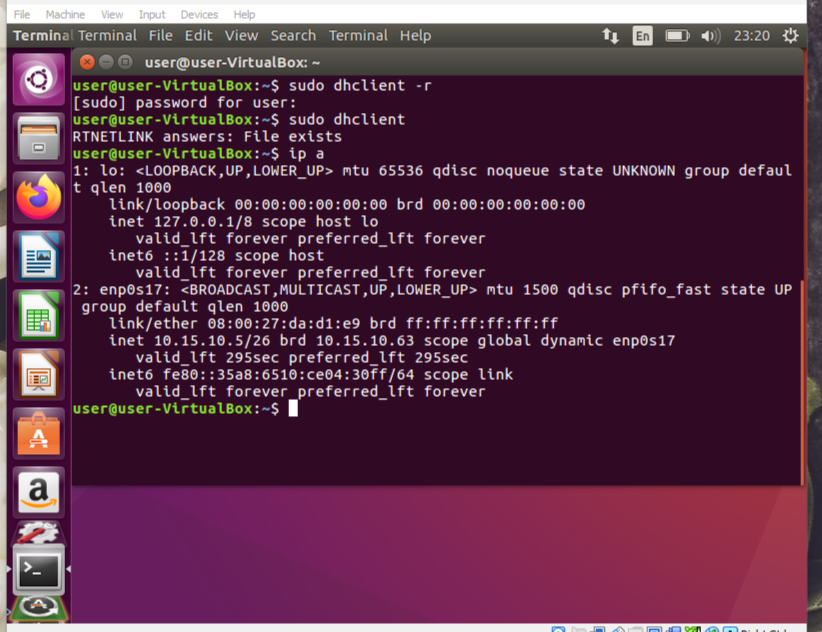
\includegraphics[width=0.65\textwidth]{02_00 (20_1)}
    \caption{Обновленные параметры сетевых интерфейсов}
    \label{img:0018}
  \end{figure}

  \subsubsection{Непосредственно спуффинг}

  Для осуществления \textit{DHCP} спуффинга запустим ранее скачанную утилиту \textit{ettercap}:

  \begin{figure}[H]
    \centering
    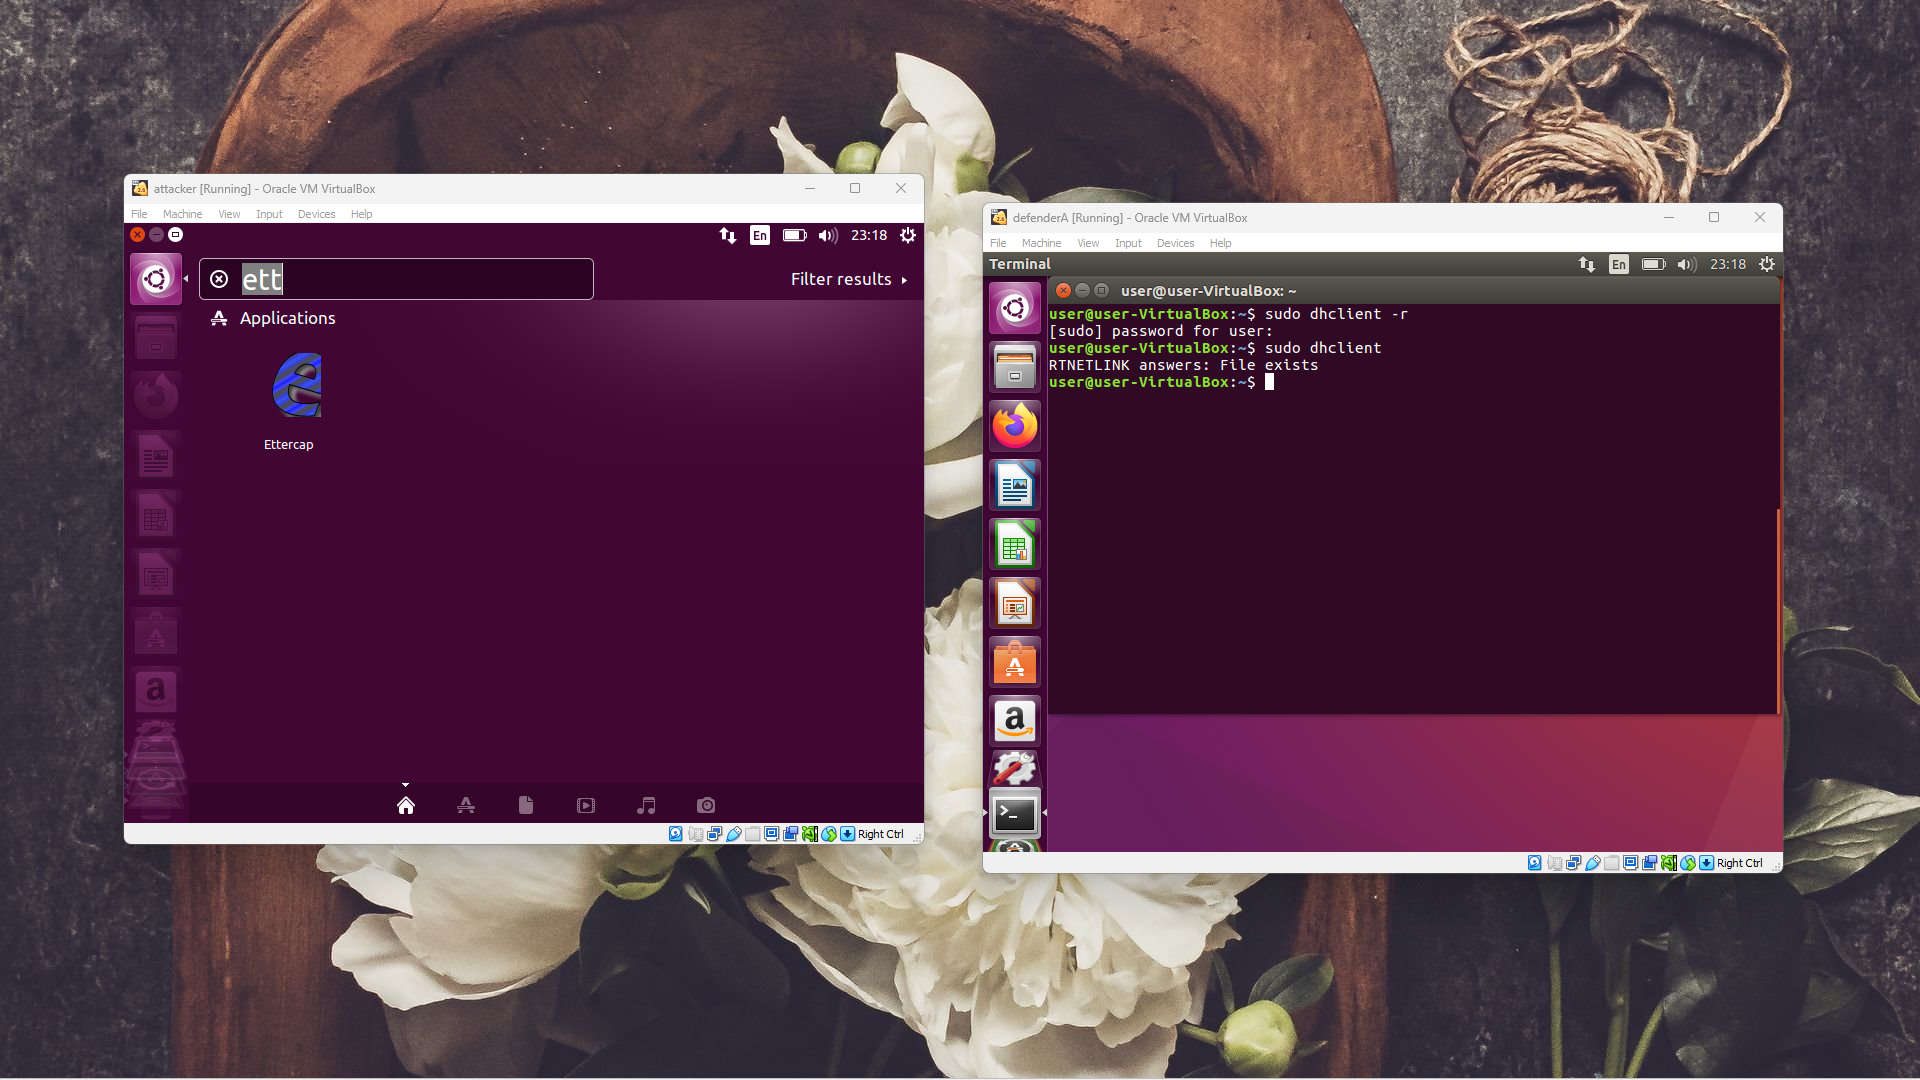
\includegraphics[width=0.85\textwidth]{02_00 (23)}
    \caption{Запускаем ettercap}
    \label{img:0019}
  \end{figure}

  Данная утилита требует права суперпользователя, поэтому выдем их, указав пароль:

  \begin{figure}[H]
    \centering
    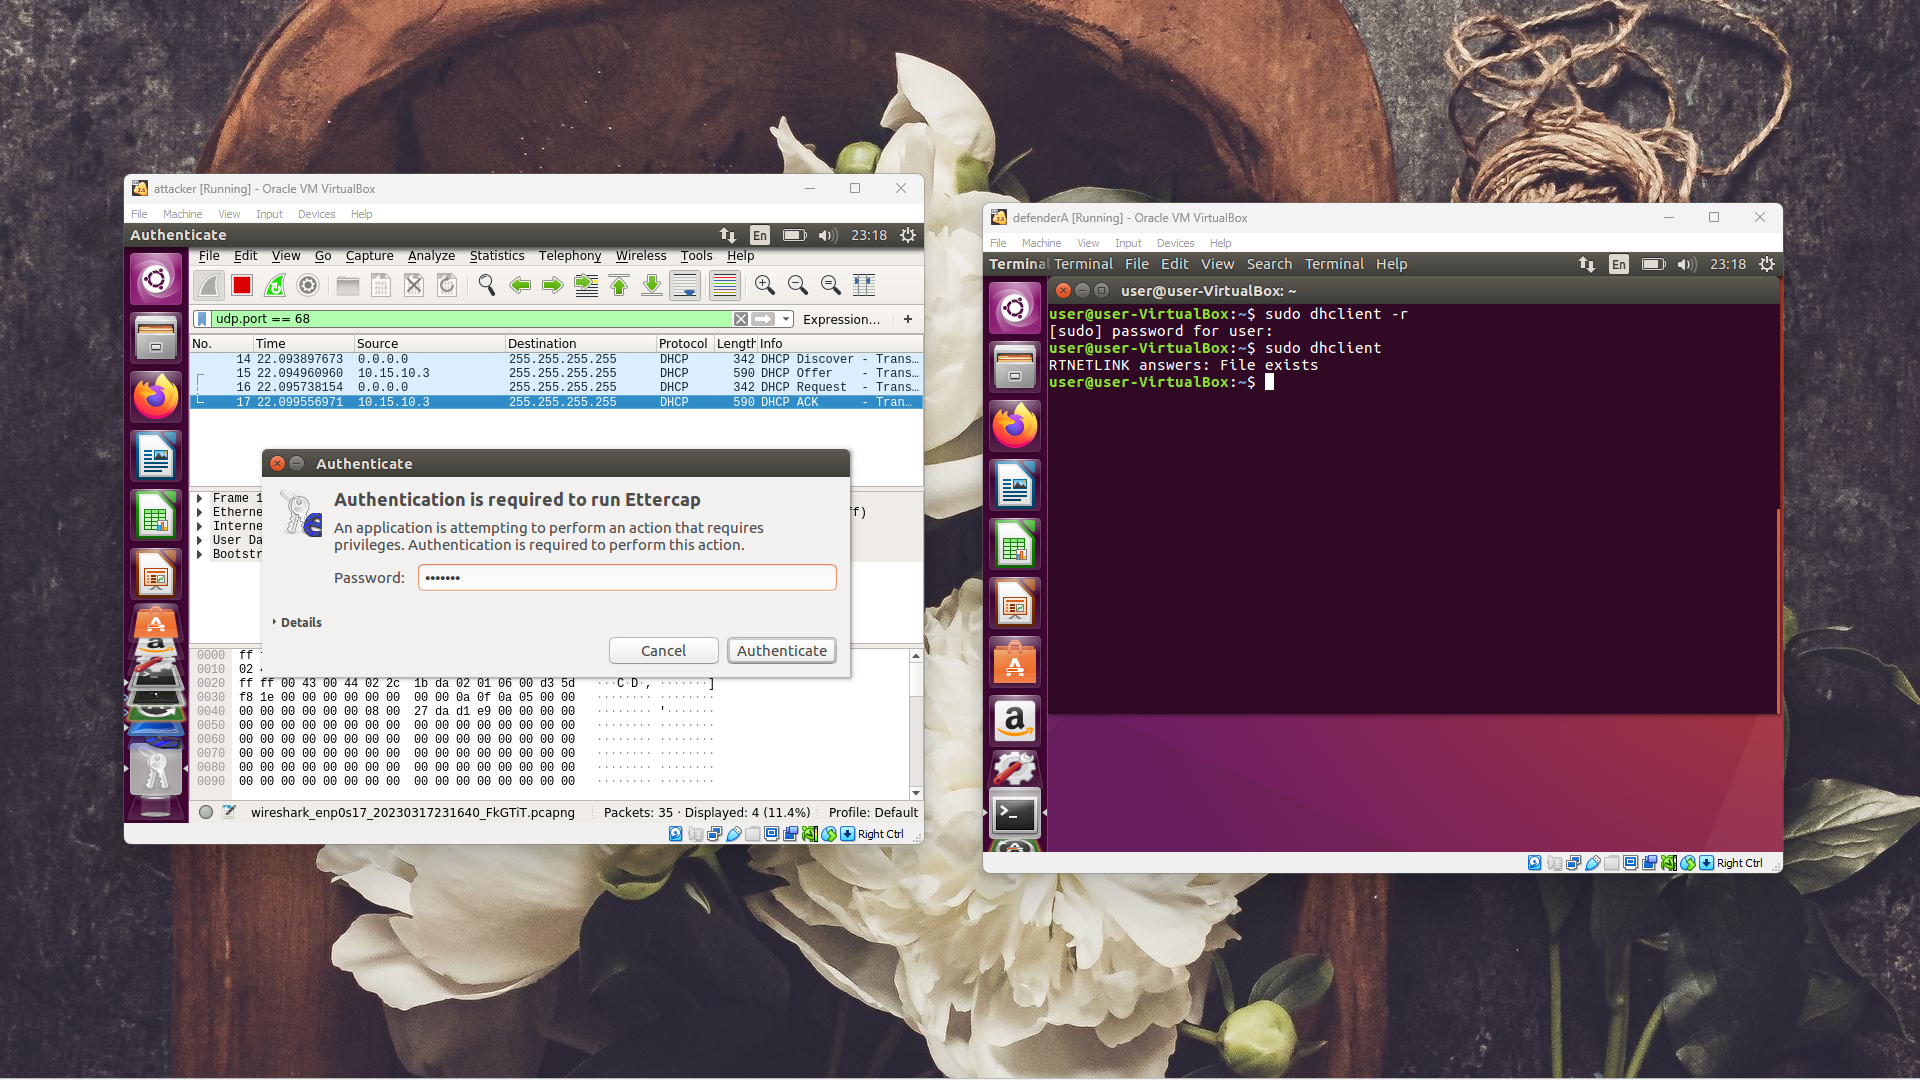
\includegraphics[width=0.85\textwidth]{02_00 (24)}
    \caption{Выдача необходимых прав}
    \label{img:0020}
  \end{figure}

  Далее идет настройка утилиты для правильной работы. Для начала укажем режим работы встроенного
  в \textit{ettercap} сниффера - в меню выбираем пункт \textbf{sniff}, а в нем уже указываем
  сам режим - \textbf{Unified Sniffing}:

  \begin{figure}[H]
    \centering
    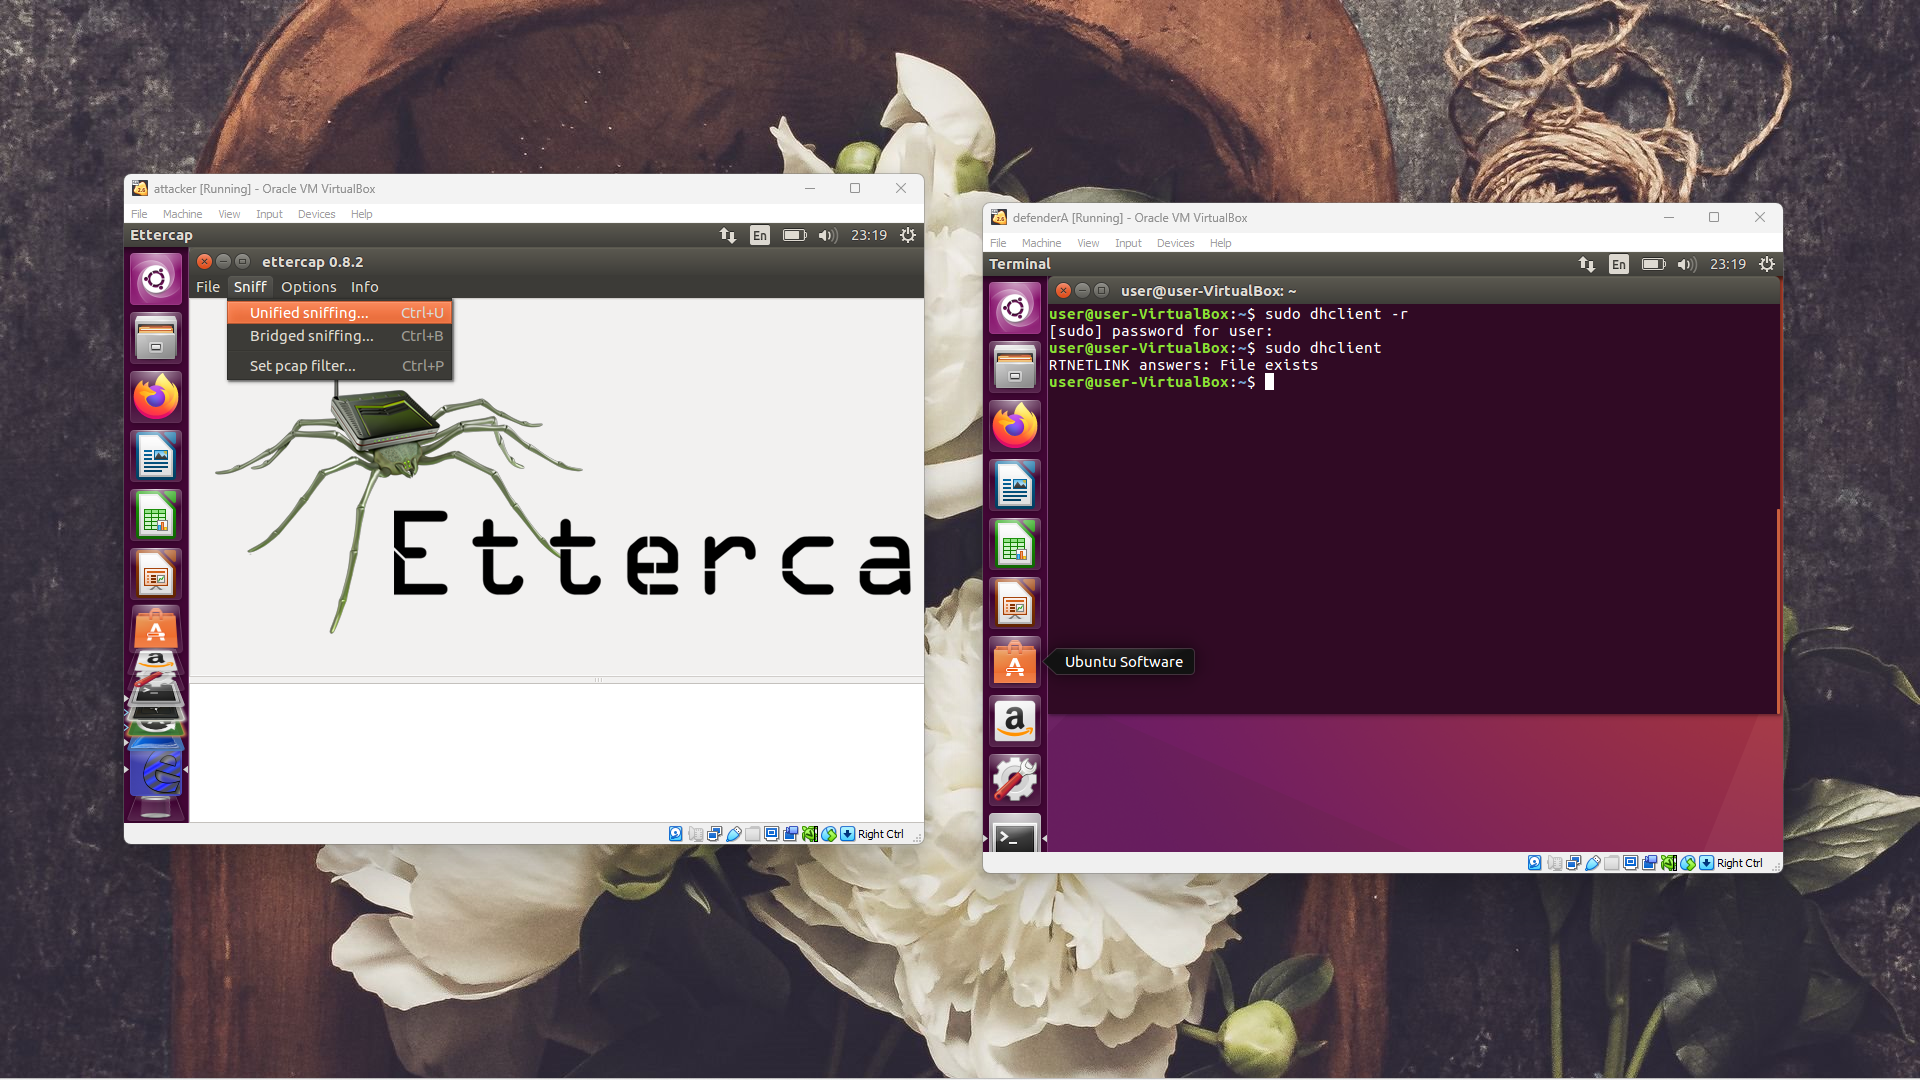
\includegraphics[width=0.85\textwidth]{02_00 (25)}
    \caption{Указываем режим сниффинга}
    \label{img:0021}
  \end{figure}

  Далее потребуется указать используемый сетевой интерфейс (для текущей машины это \textit{enp0s17}):

  \begin{figure}[H]
    \centering
    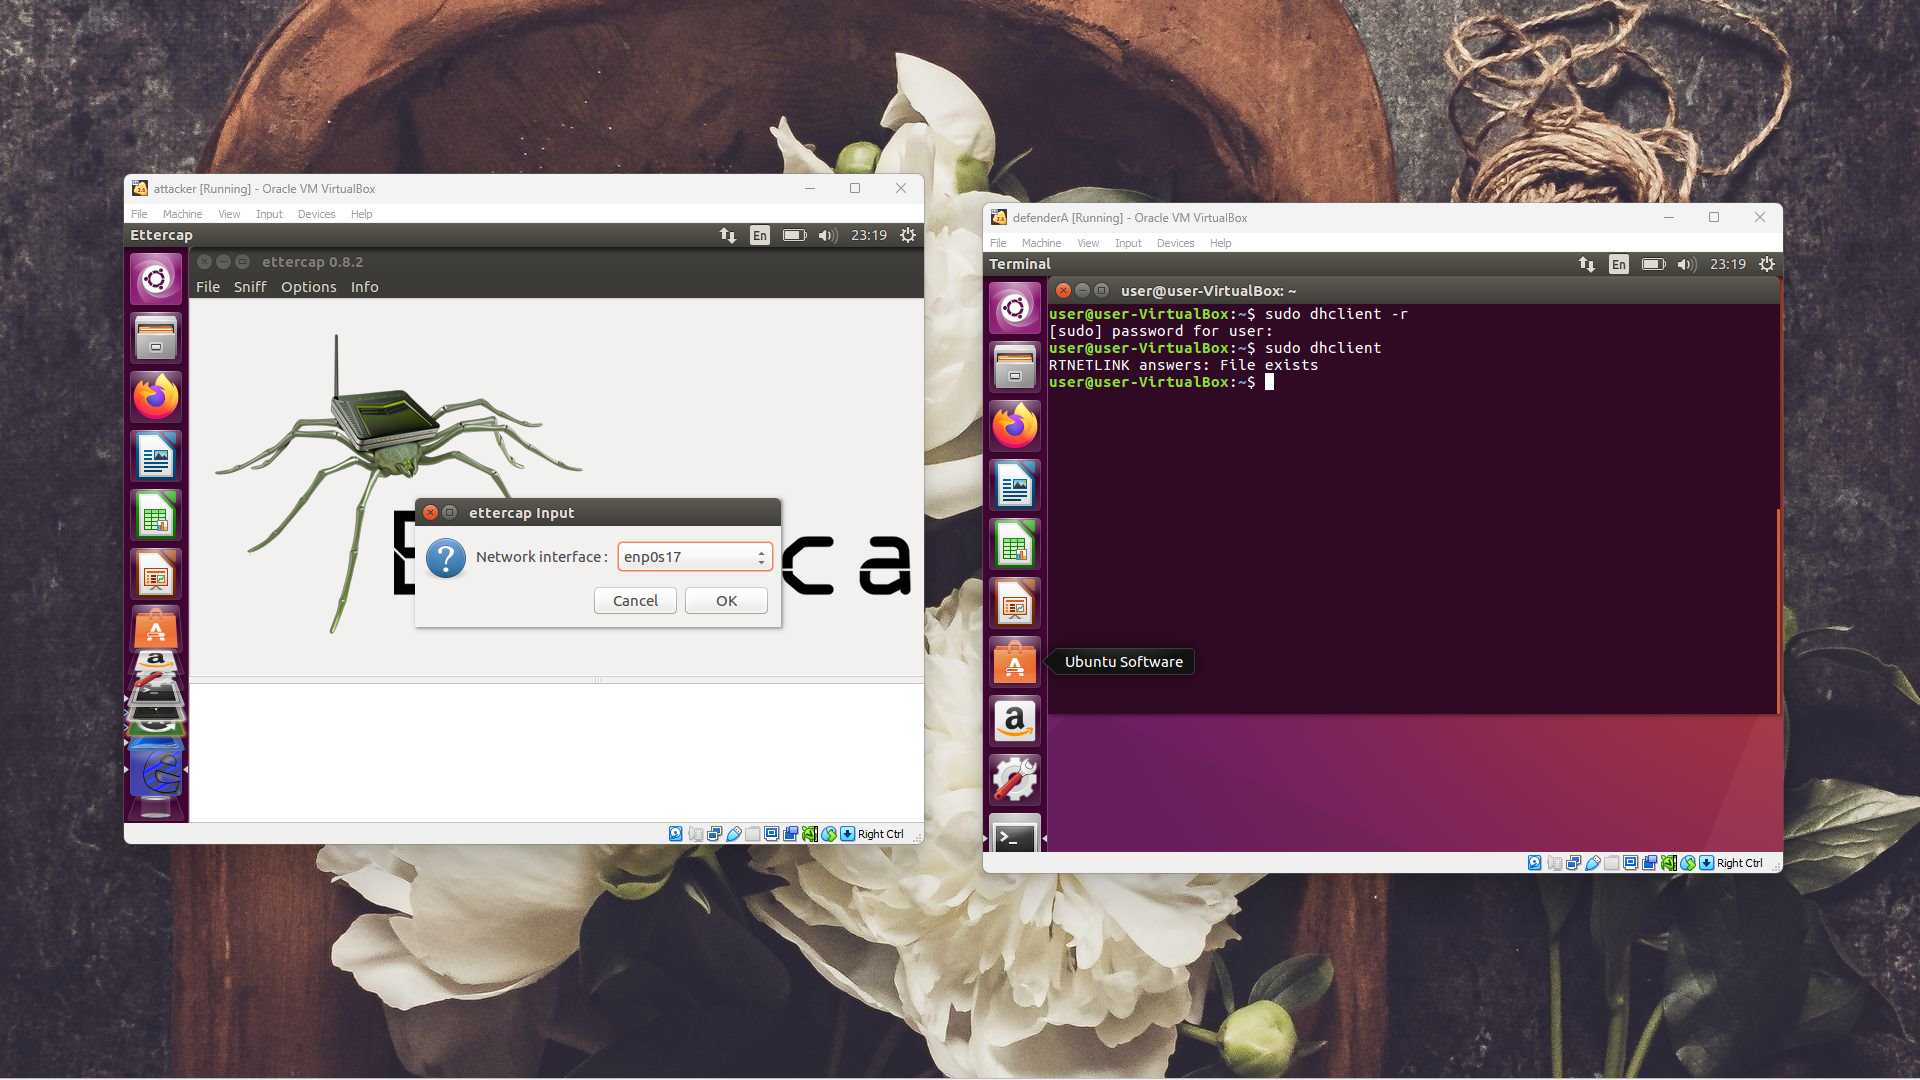
\includegraphics[width=0.85\textwidth]{02_00 (26)}
    \caption{Выбираем нужный сетевой интерфейс}
    \label{img:0022}
  \end{figure}

  Далее запускаем необходимую нам \textit{MITM}-атаку, для этого в меню \textbf{Mitm}
  выбираем пункт \textbf{DHCP Spoofing}:

  \begin{figure}[H]
    \centering
    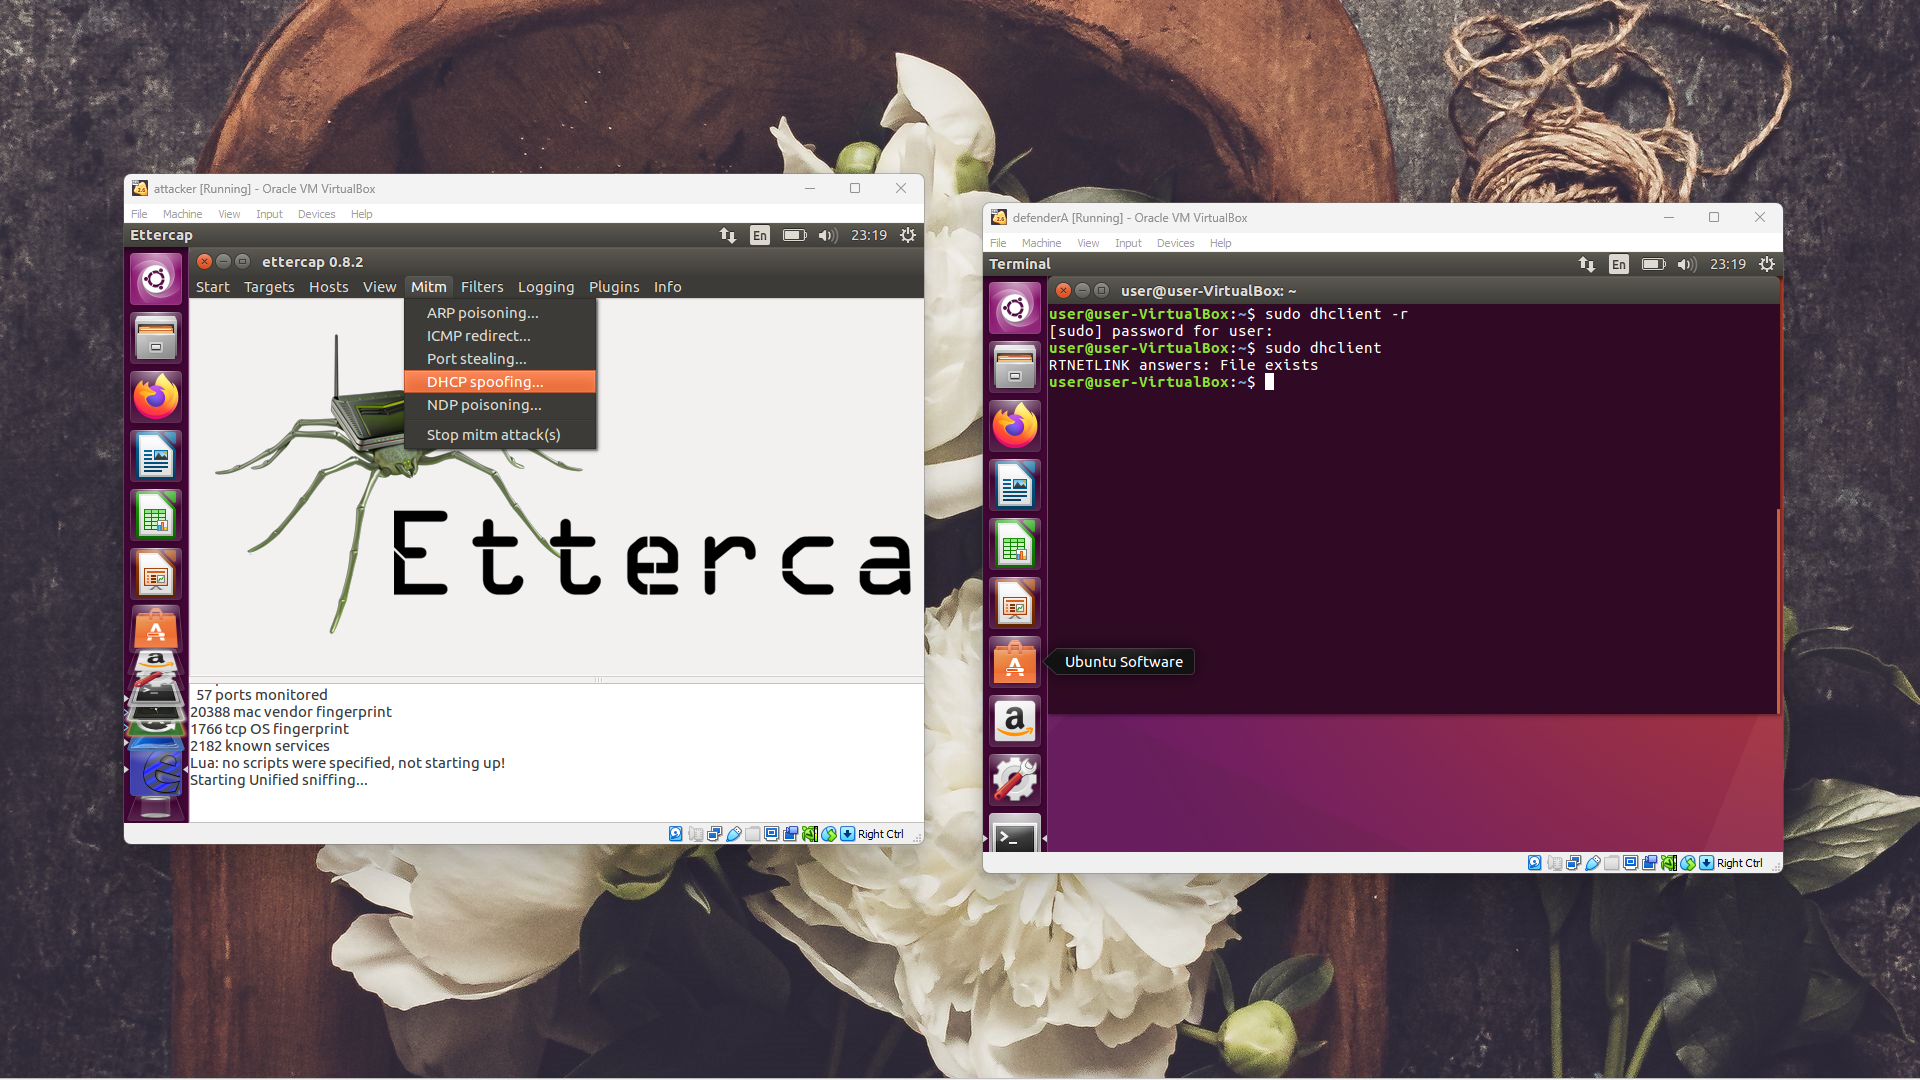
\includegraphics[width=0.85\textwidth]{02_00 (27)}
    \caption{Запуск DHCP спуффинга}
    \label{img:0023}
  \end{figure}

  Саму атаку опять таки придется настроить:

  \begin{figure}[H]
    \centering
    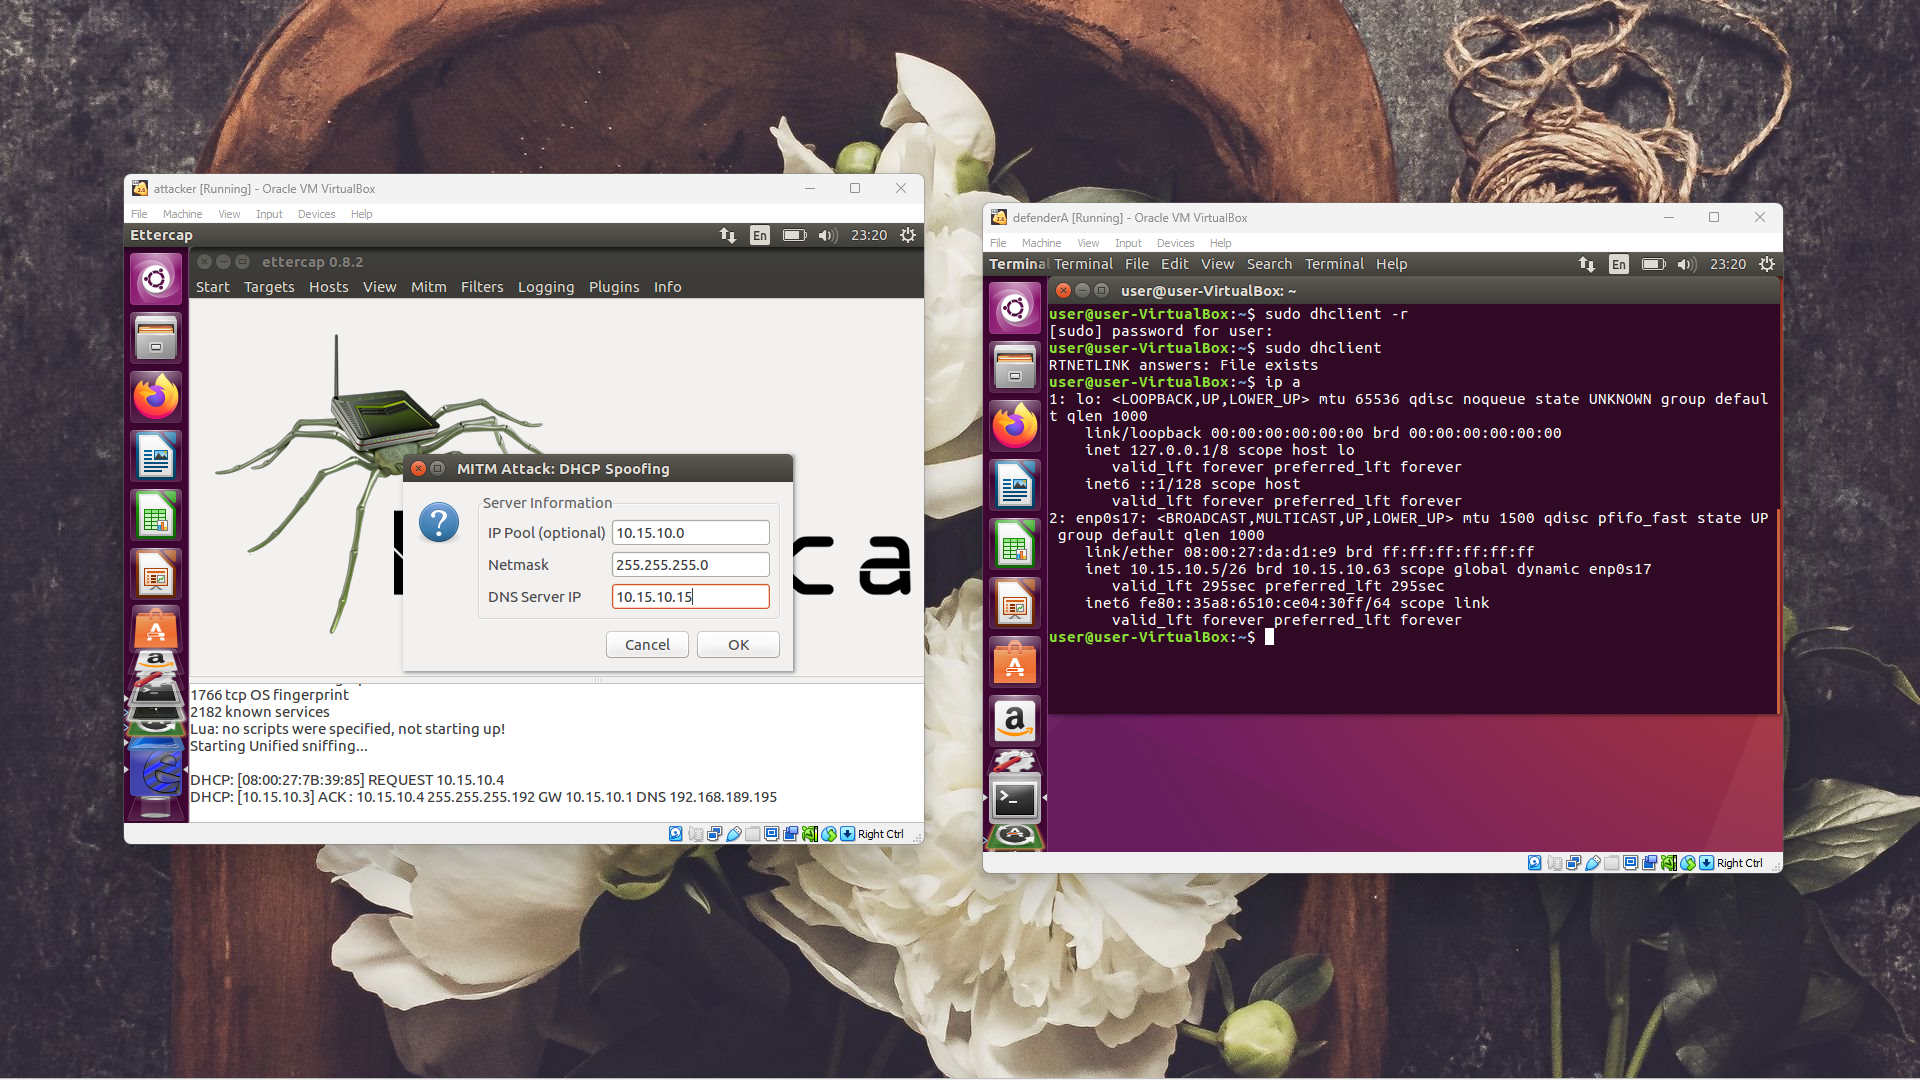
\includegraphics[width=0.85\textwidth]{02_00 (28)}
    \caption{Настройка спуффинга}
    \label{img:0024}
  \end{figure}

  Здесь \textit{IP Pool} - адрес сети, \textit{Netmask} - маска сети. Их значения 
  не соотвествуют реальным (в действительности используемым). Поле \textit{DNS Server IP} -
  адрес \textit{DNS} сервера, который необходимо предлагать при отправке \textit{DHCP Offer} пакета
  (в конкретном случае он отличается от реального - 10.15.10.1). 

  Нажимем \textit{OK} - спуффинг запущен, необходимо проверить, что все работает. Для этого
  опять сбросим и запросим новый \textit{IP} адрес для атакуемой машины (при помощи того же \textit{dhclient}):

  \begin{figure}[H]
    \centering
    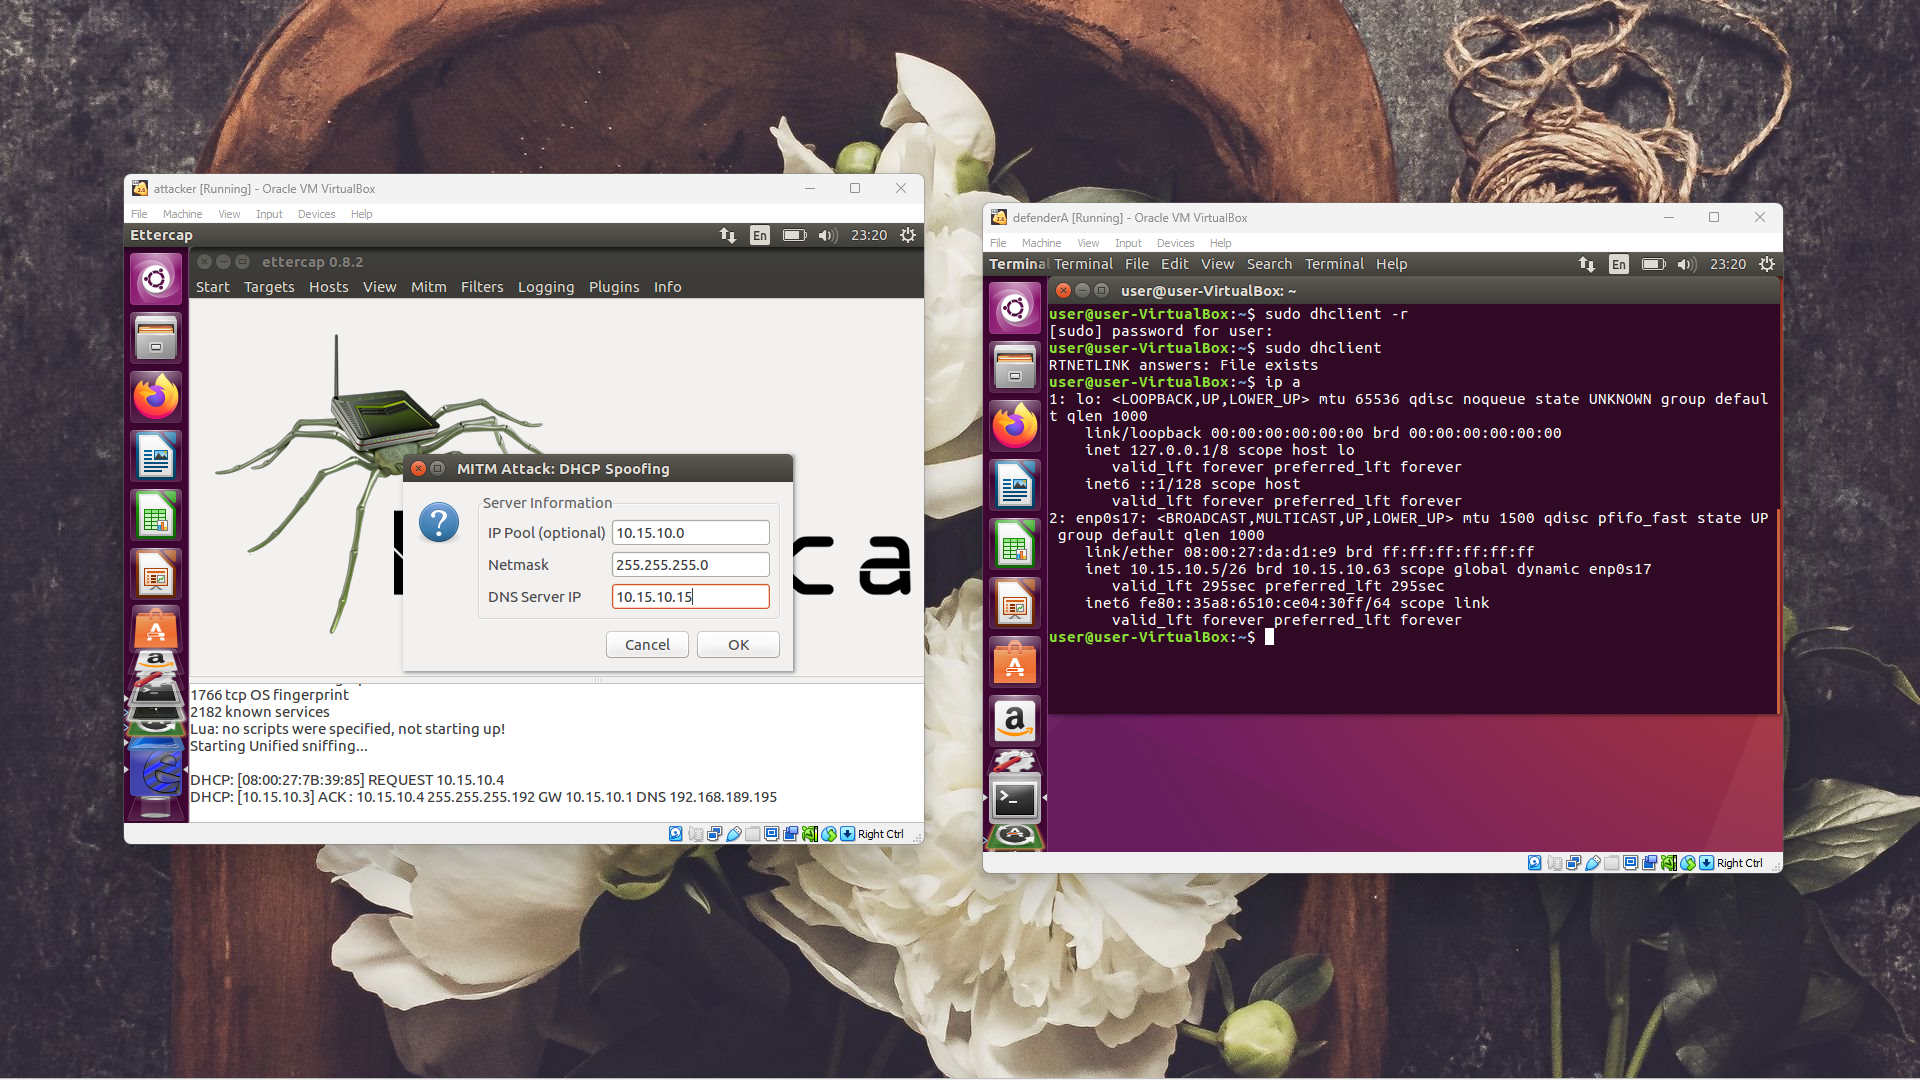
\includegraphics[width=0.85\textwidth]{02_00 (28)}
    \caption{Атакуемая машина попала в ловушку}
    \label{img:0025}
  \end{figure}

  В окне \textit{ettercap} видно сообщение о том, что ловушка сработала, чего мы и добавлись.
  Теперь рассмотрим перехваченные во время атаки сетевые пакеты:

  \begin{figure}[H]
    \centering
    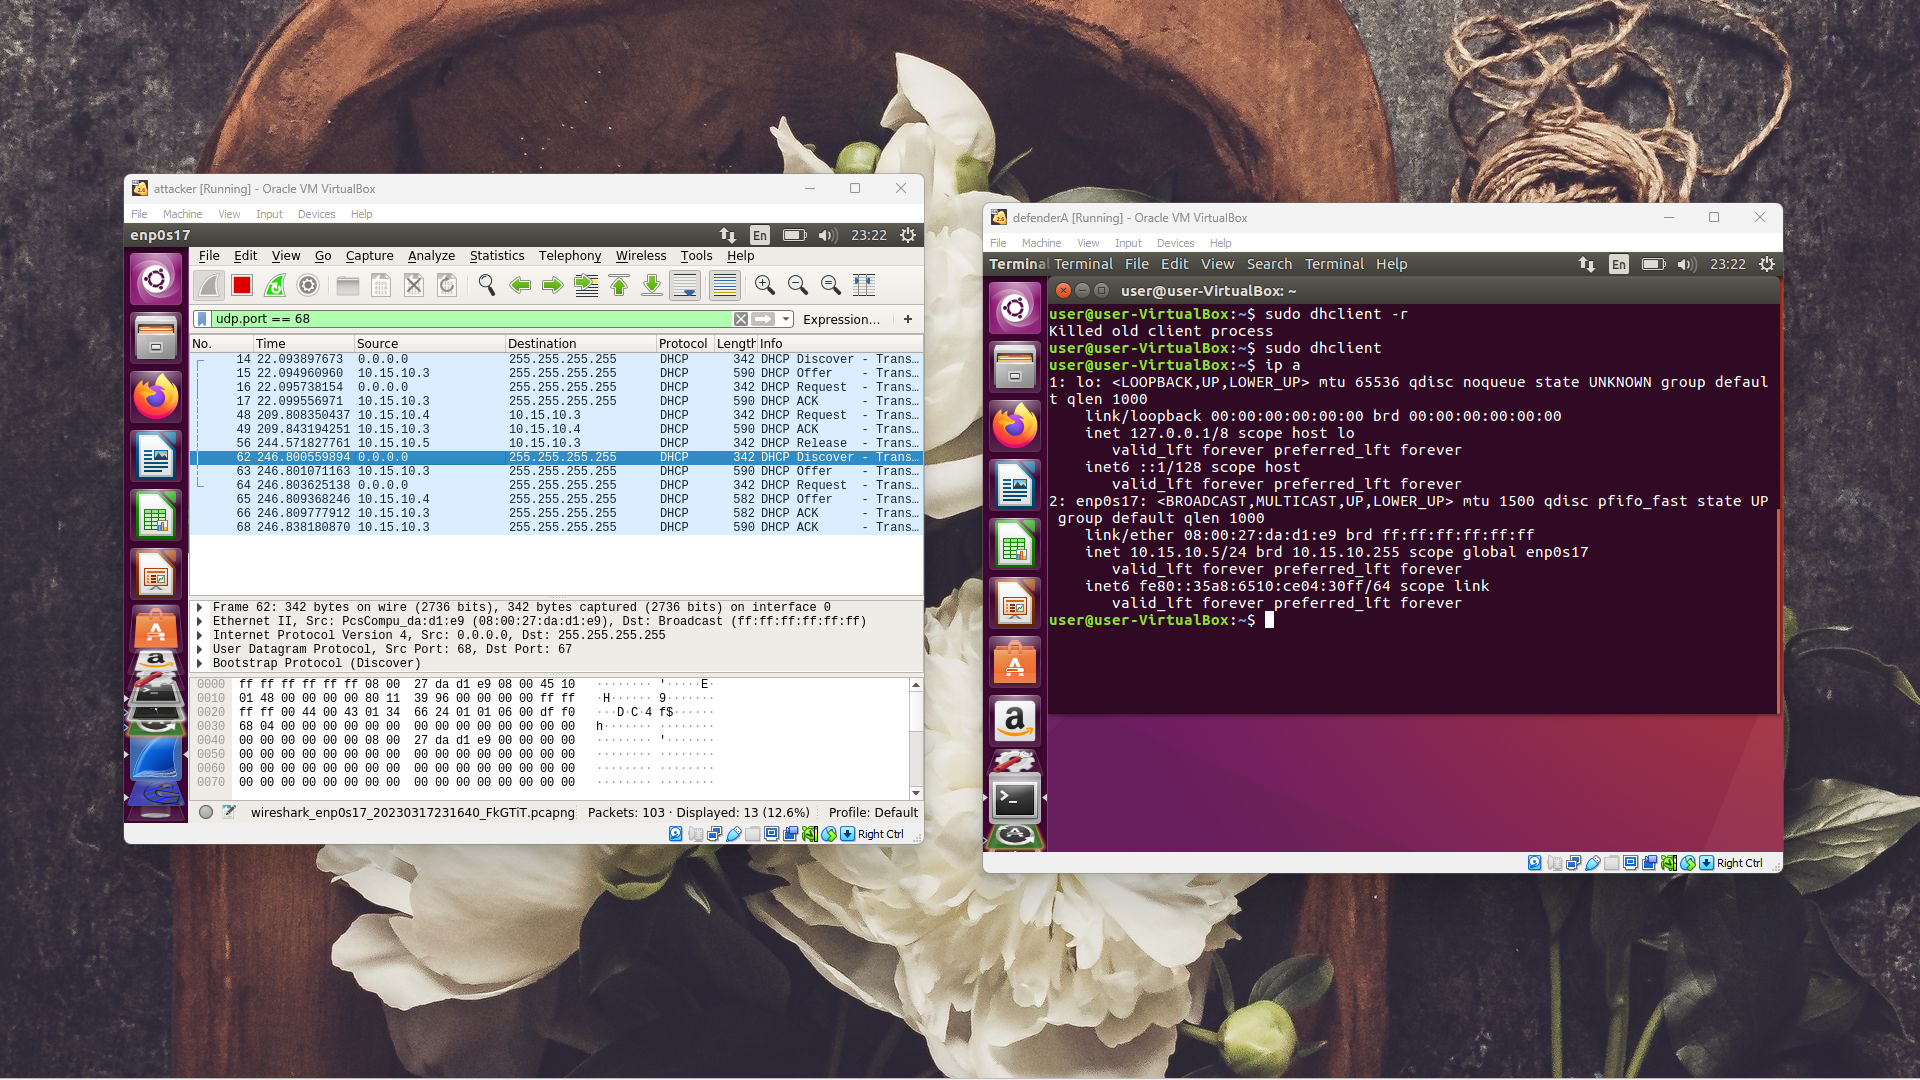
\includegraphics[width=0.85\textwidth]{02_00 (32)}
    \caption{Перехваченные пакеты}
    \label{img:0026}
  \end{figure}

  В первую очередь атакуемая машина освободила ранее присвоенный ей адрес при помощи
  \textit{DHCP RELEASE} широковещательного запроса. Далее она опять отправила \textit{DHCP Discover},
  чтобы узнать информацию о текущей сети (адреса \textit{DHCP} и \textit{DNS}-серверов и т.п.).

  Однако на этот раз атакуемая машина получила не один, а целых два \textit{DHCP Offer} ответа.
  Это произошло потому, что запущенный спуффер правильно отработал - подменил реальный ответ на свой,
  содержащий отравленный адрес \textit{DNS}-сервера.

  Из полученной ранее информации известно, что адрес реального \textit{DHCP}-сервера соответсвует
  10.15.10.3, что говорит о том, что пакеты, отправленные с другого адрес - пакеты, отправленные спуффером.

  Рассмотрим Offer, полученный от атакующей машины:

  \begin{figure}[H]
    \centering
    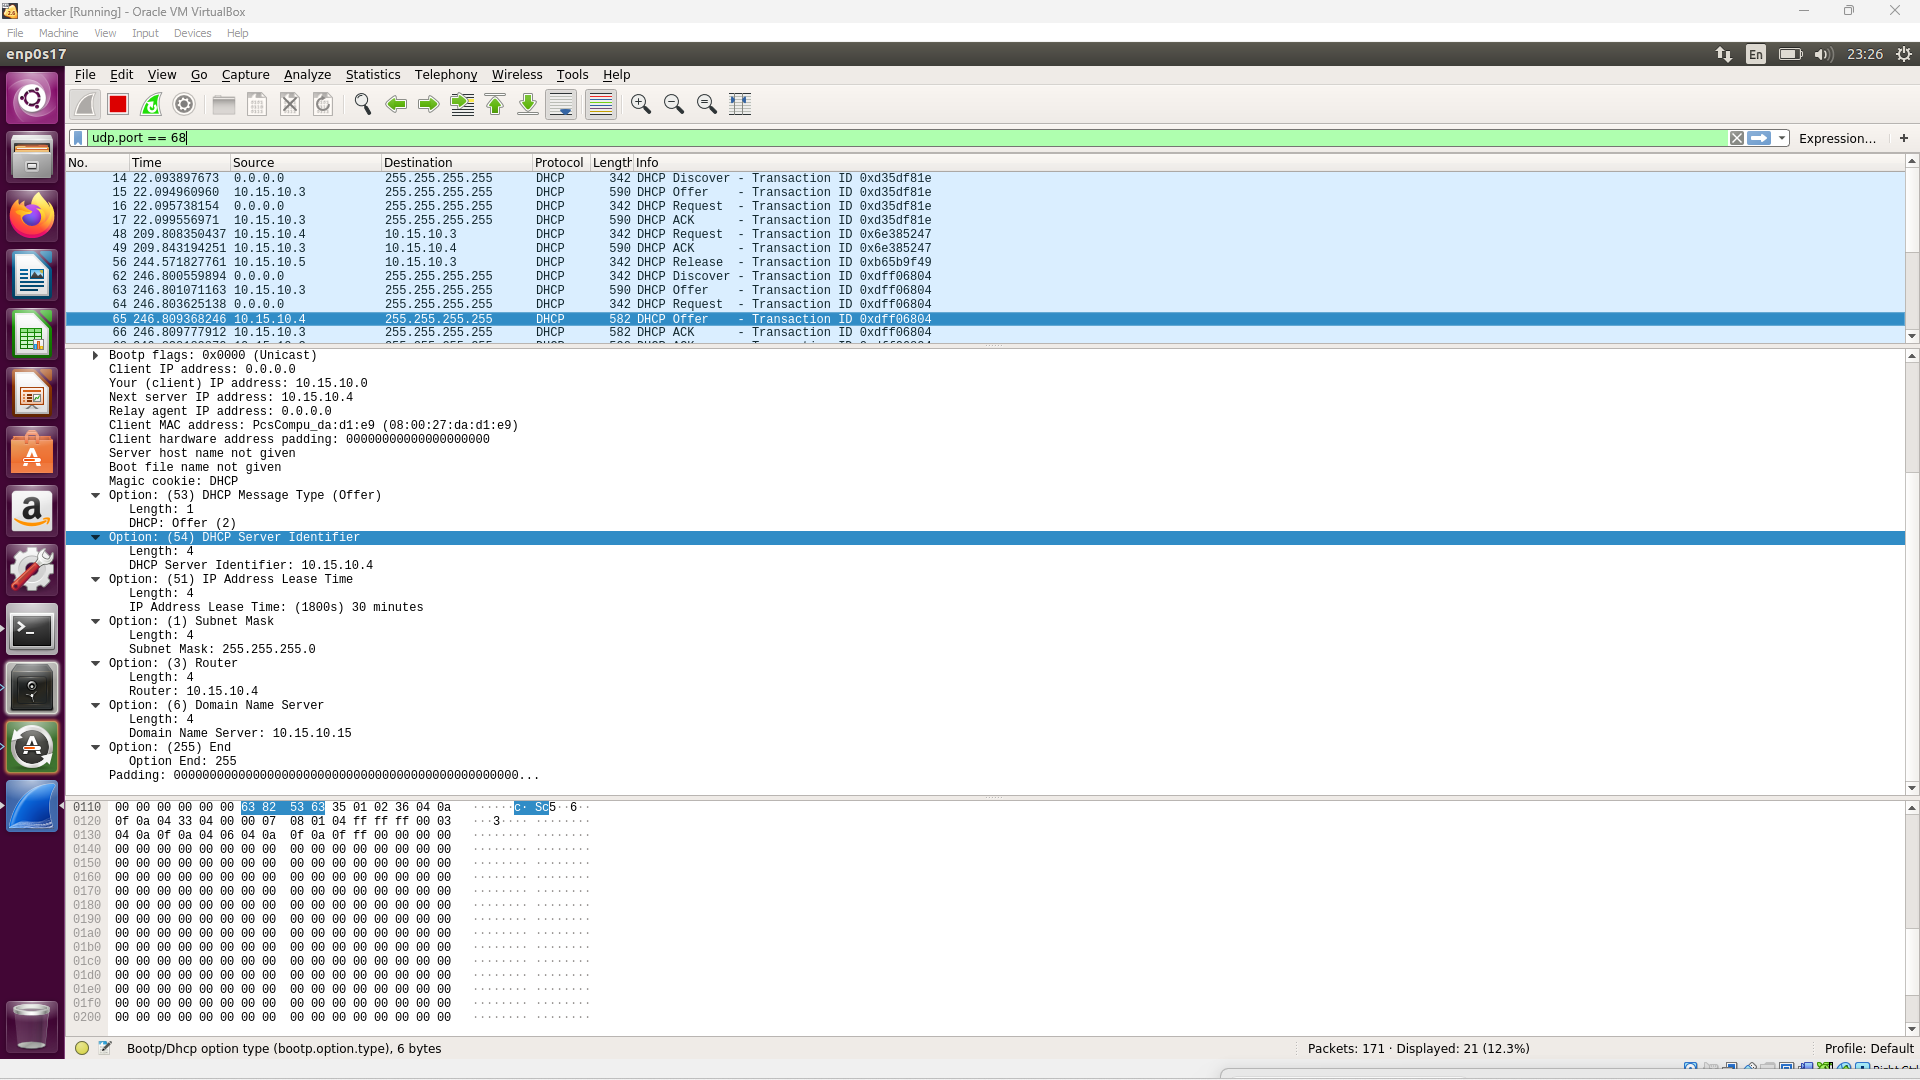
\includegraphics[width=0.85\textwidth]{02_00 (37)}
    \caption{Отравленный DHCP Offer}
    \label{img:0027}
  \end{figure}

  Видно, что данный ответ отдает неправильные адреса сети, \textit{DHCP} и \textit{DNS} серверов.
  Если посмотреть на вывод команды \textit{ip a} на рис. \ref{img:0018} на стр. \pageref{img:0018},
  а потом на вывод той же команды на рис. \ref{img:0026} на стр. \pageref{img:0026}, то видно,
  что спуффинг сработал и данные скомпрометированны.

  \subsubsection{Очистка}

  Чтобы сбросить результаты атаки перезагрузим обе ВМ:

  \begin{figure}[H]
    \centering
    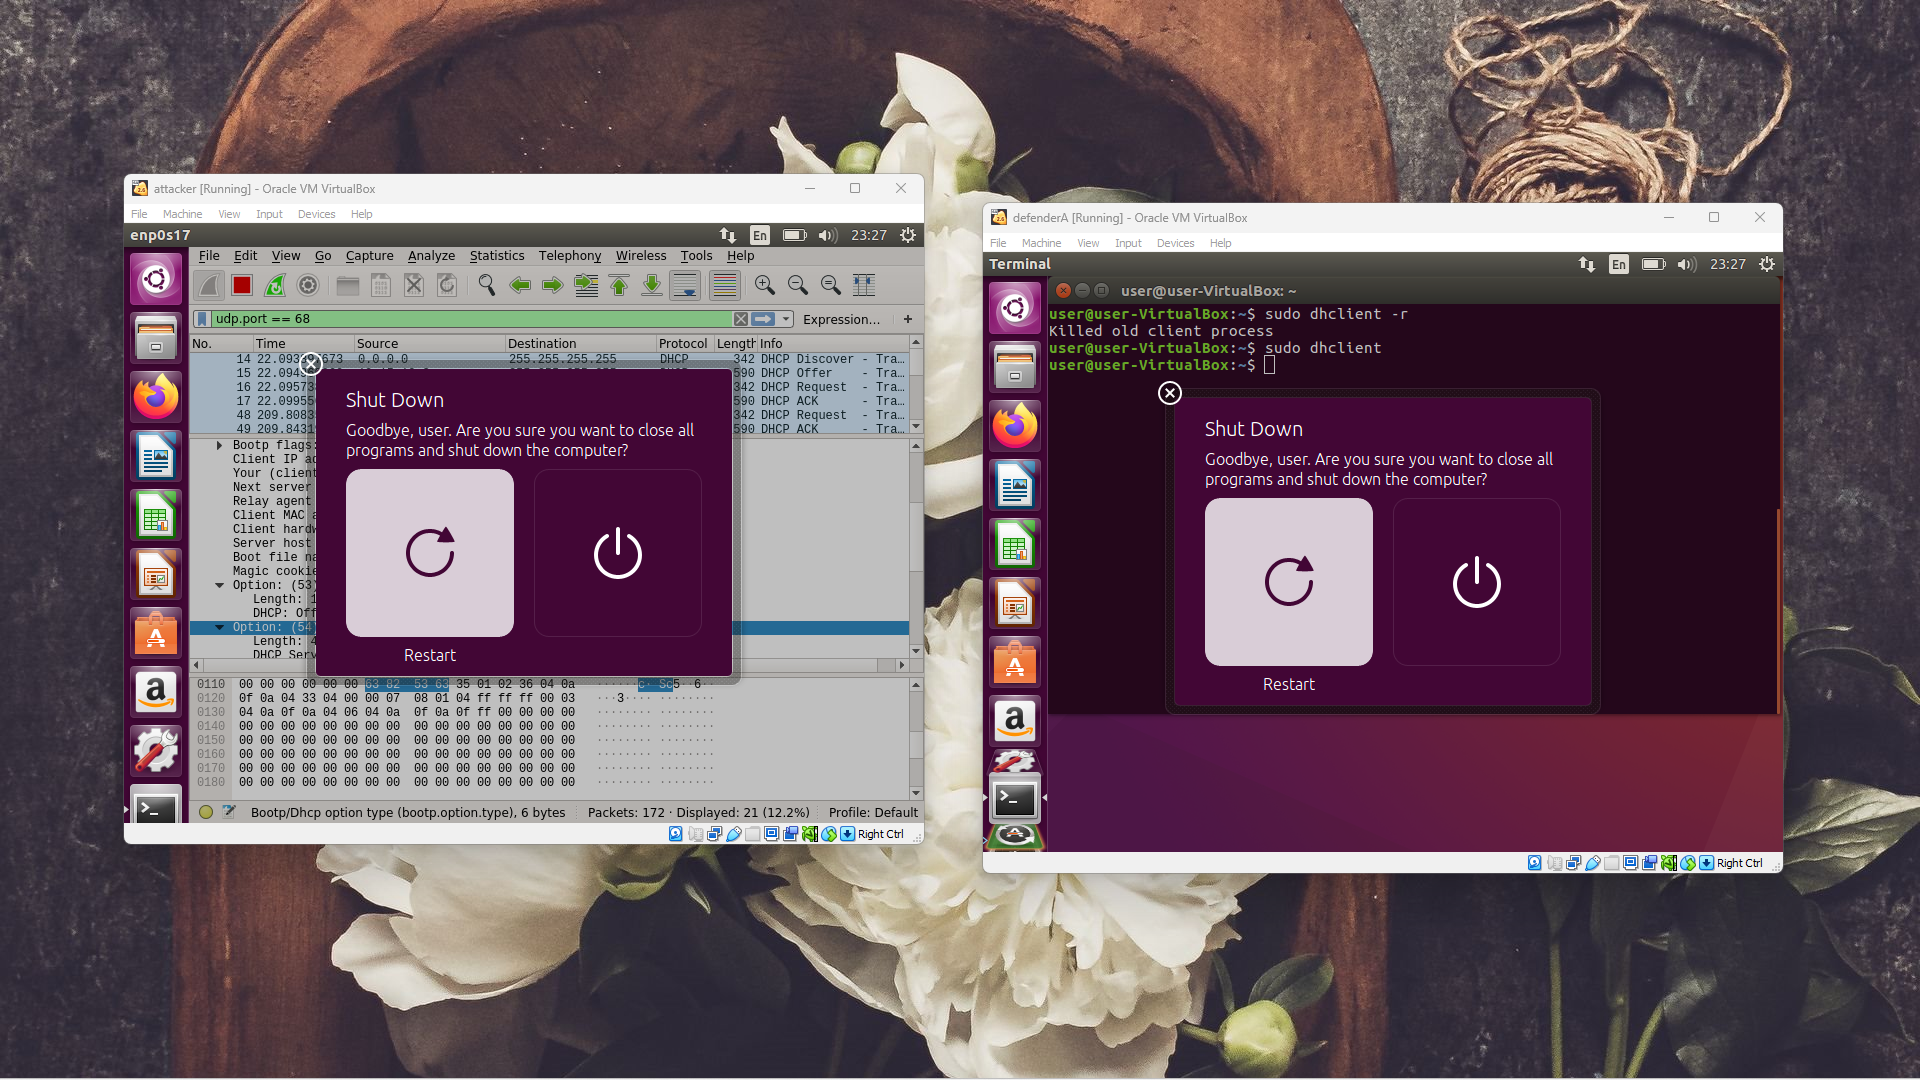
\includegraphics[width=0.85\textwidth]{02_00 (38)}
    \caption{Перезагрузка виртуальных машин}
    \label{img:0028}
  \end{figure}

  \subsection{ARP-spoofing}
  \subsubsection{Подготовка к атаке}

  Для осуществления этой атаки нам потребуется еще одна атакуемая машина, создадим ее
  при помощи клонирования уже существующей:

  \begin{figure}[H]
    \centering
    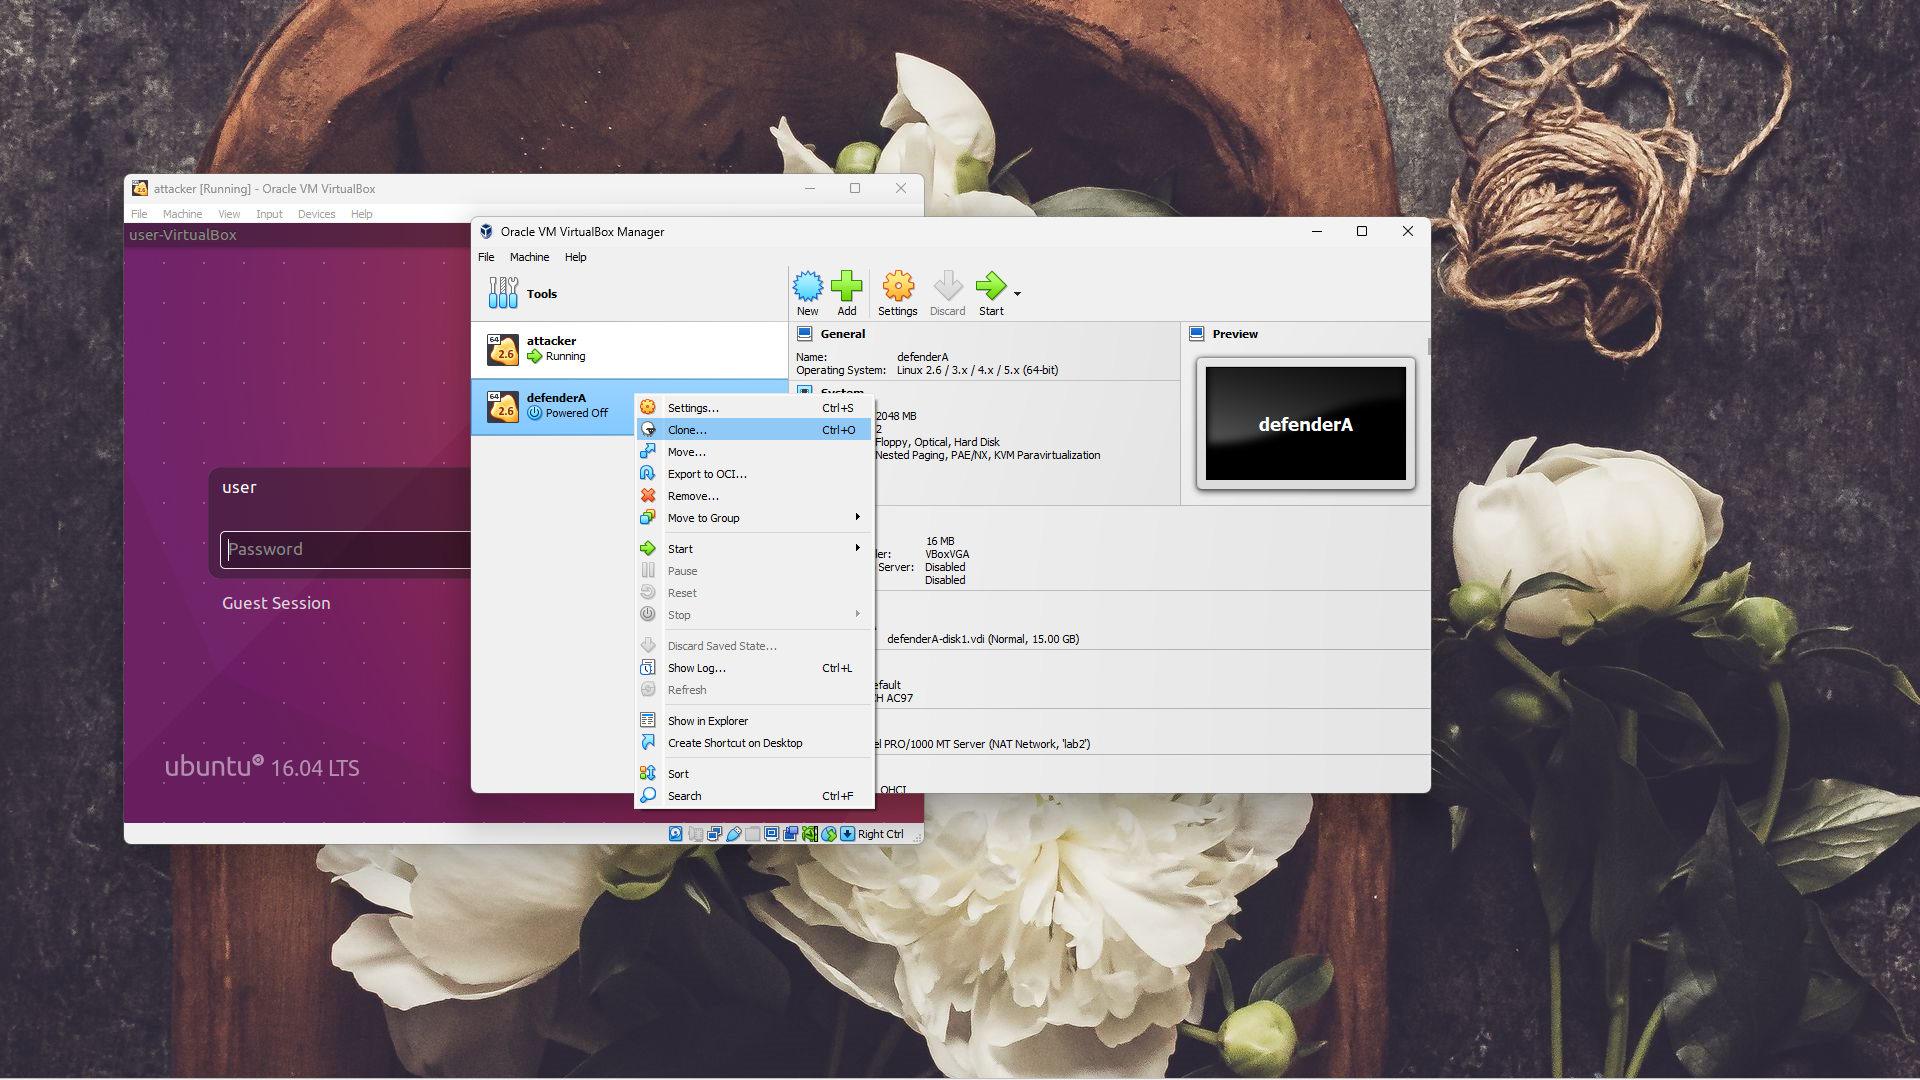
\includegraphics[width=0.85\textwidth]{02_00 (39)}
    \caption{Запускаем клонирование ВМ}
    \label{img:0029}
  \end{figure}

  \begin{figure}[H]
    \centering
    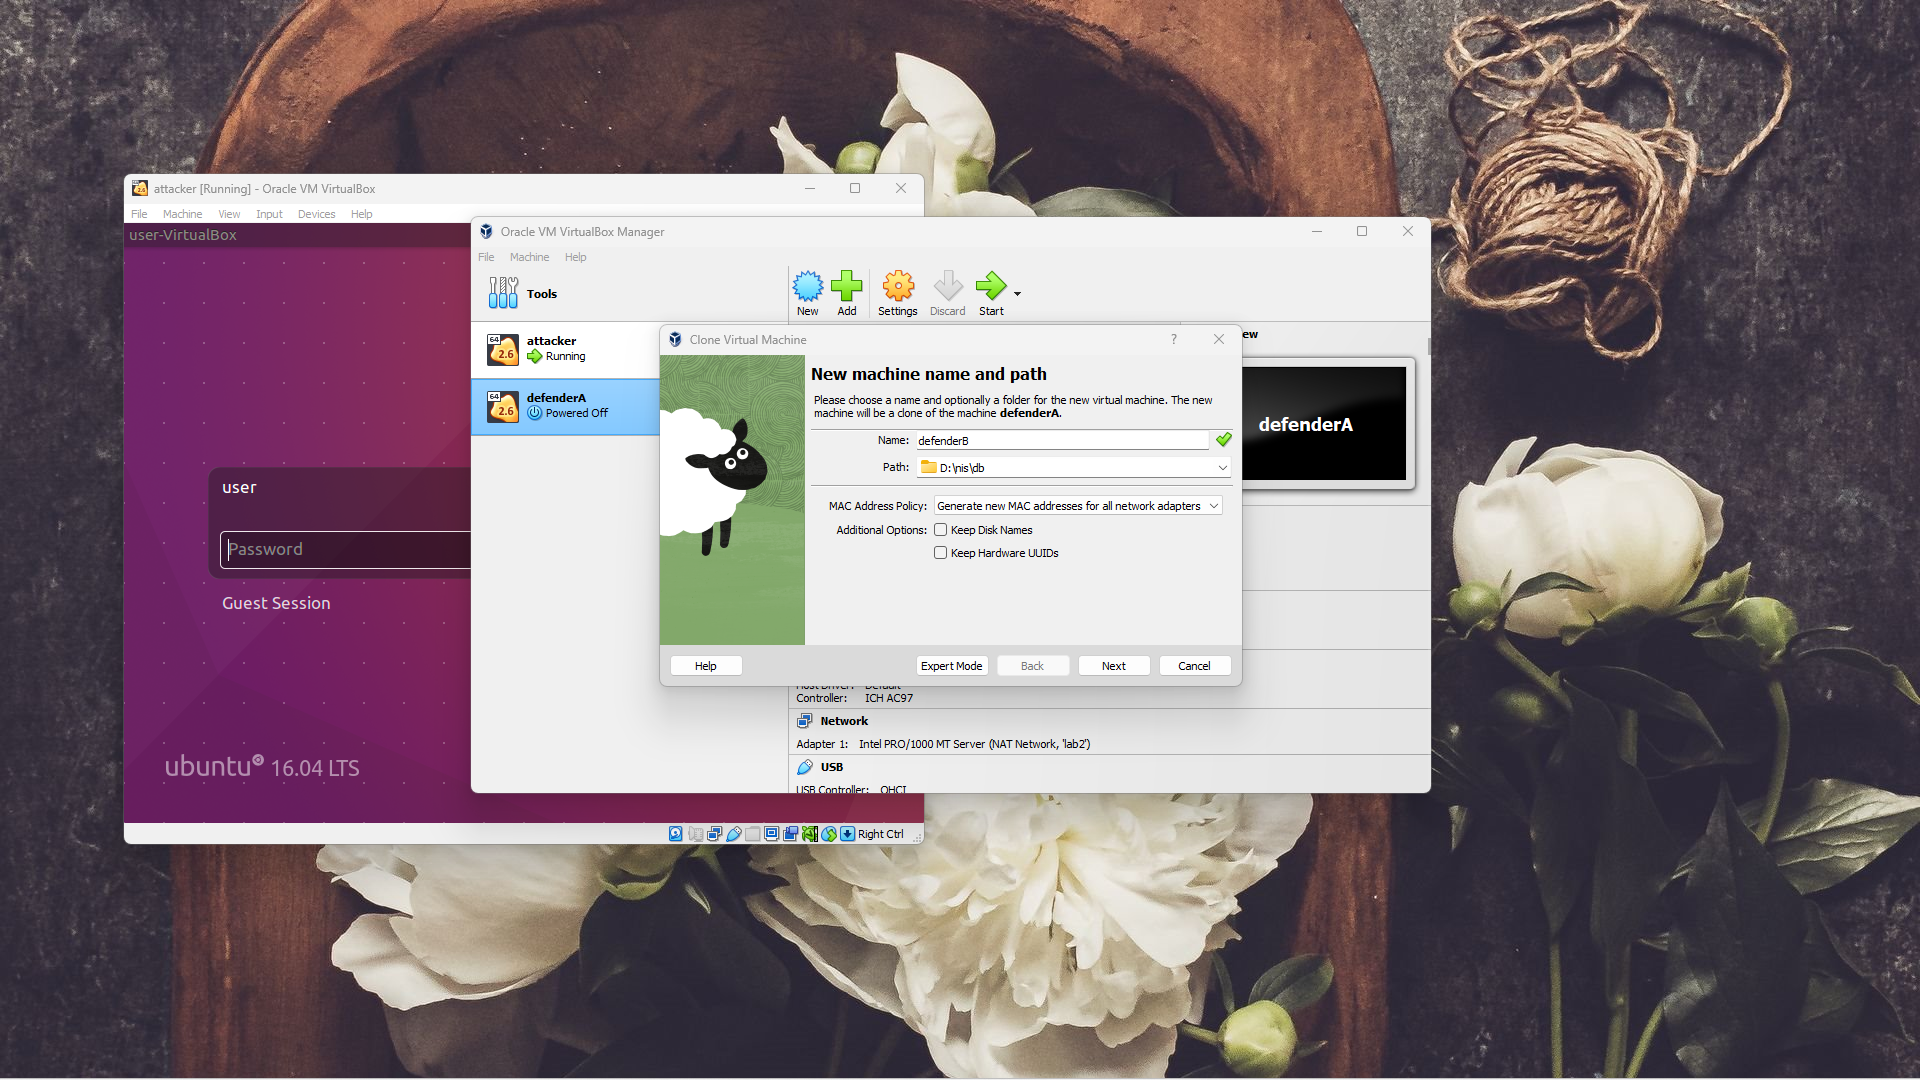
\includegraphics[width=0.85\textwidth]{02_00 (40)}
    \caption{Указываем ее имя и расположение}
    \label{img:0030}
  \end{figure}

  Итого - имеется одна атакующая машина (\textit{Attacker}) и две атакуемые (\textit{DefenderA} и \textit{DefenderB}):

  \begin{figure}[H]
    \centering
    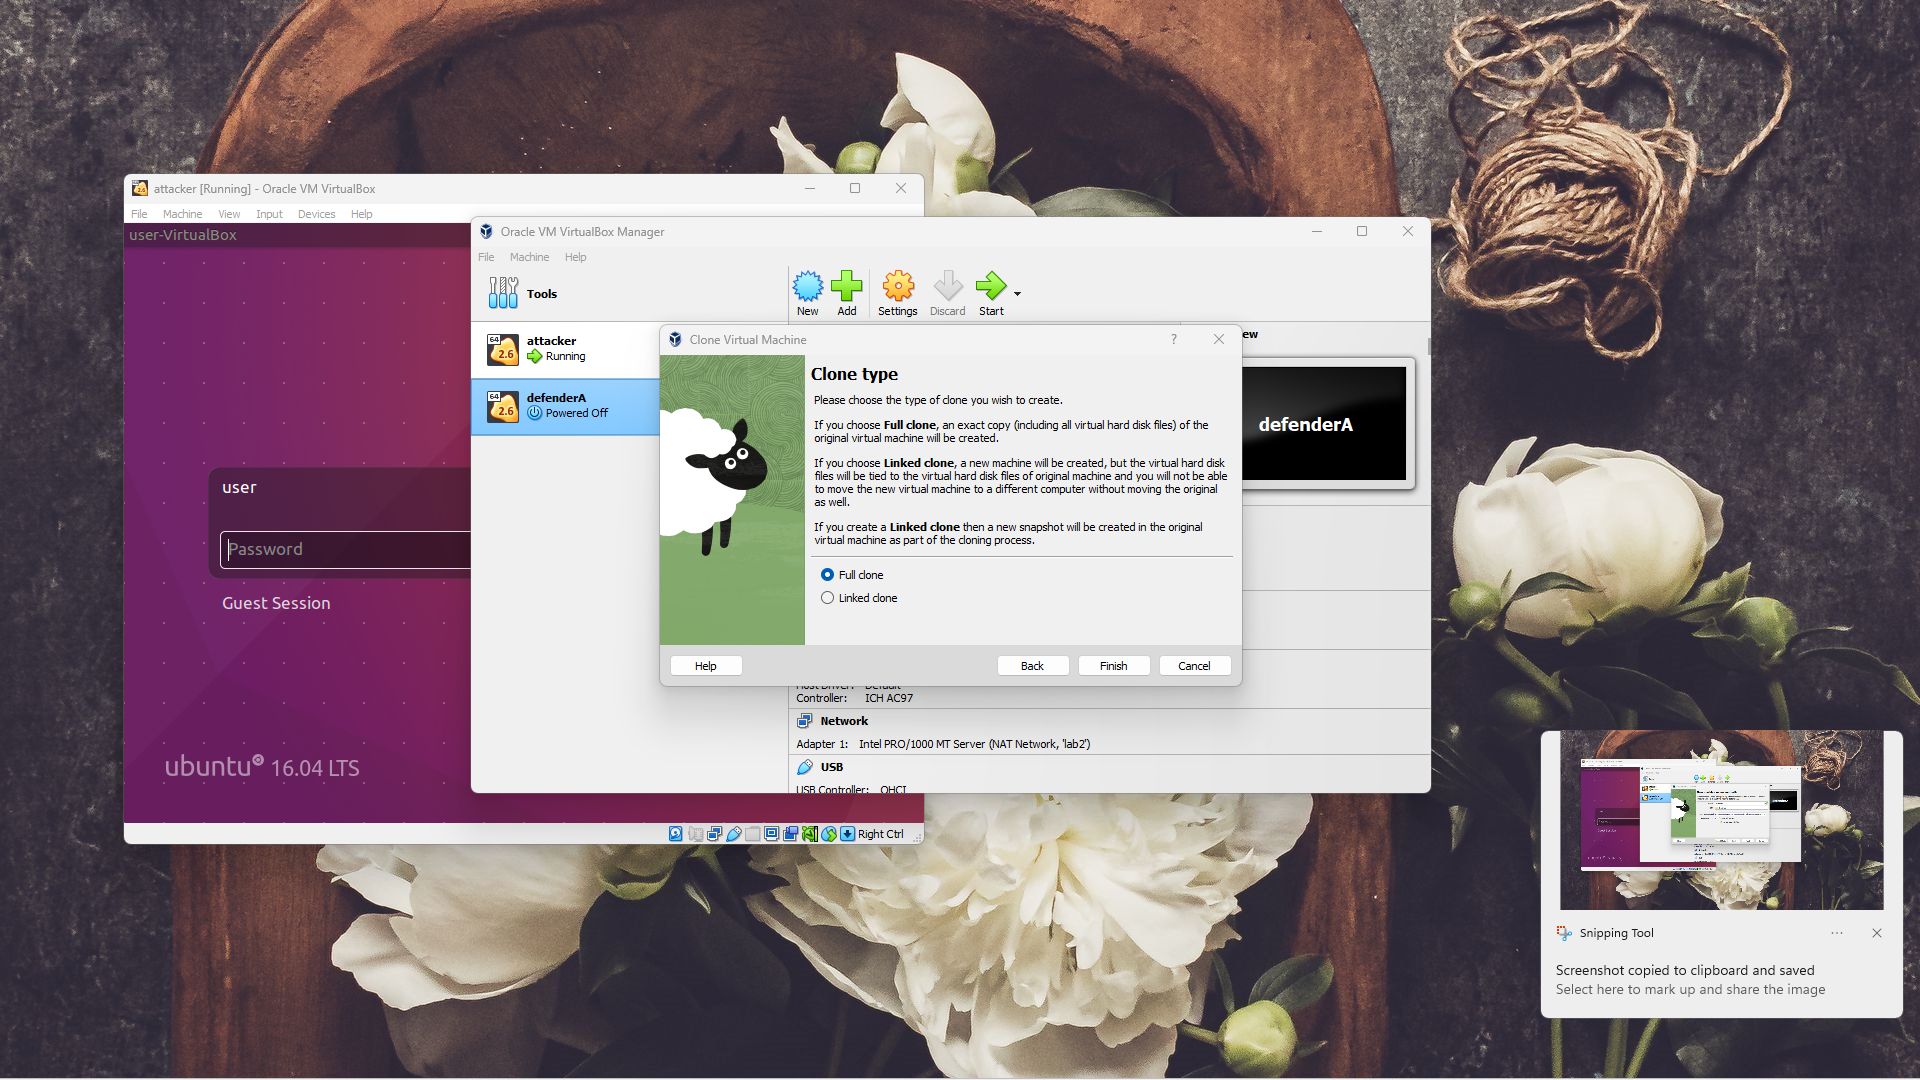
\includegraphics[width=0.85\textwidth]{02_00 (41)}
    \caption{Полученные виртуальные машины}
    \label{img:0031}
  \end{figure}

  Запускаем все виртуальные машины и узнаем их сетевые характеристики при помощи утилиты \textit{ip}:

  \begin{table}[H]
    \centering
    \begin{tabular}{| c | c | c | c | c |}
      \hline
      Имя ВМ & Статут & Сетевой интерфейс & MAC-адрес & IPv4-адрес \\
      \hline
      Attacker & Атакующий & enp0s17 & 08:00:27:7b:39:85 & 10.15.10.4 \\
      \hline
      DefenderA & Атакуемый & enp0s17 & 08:00:27:da:d1:e9 & 10.15.10.5 \\
      \hline
      DefenderB & Атакуемый & enp0s17 & 08:00:27:ab:ff:28 & 10.15.10.6 \\
      \hline
    \end{tabular}
    \caption{Информация о сетвых параметрах машин}
  \end{table}

  Далее необходимо удостовериться, что каждая из машин может по сети подключится к любой другой,
  для этого осуществим перекрестную проверку с помощью \textit{ping}:
  
  \begin{figure}[H]
    \centering
    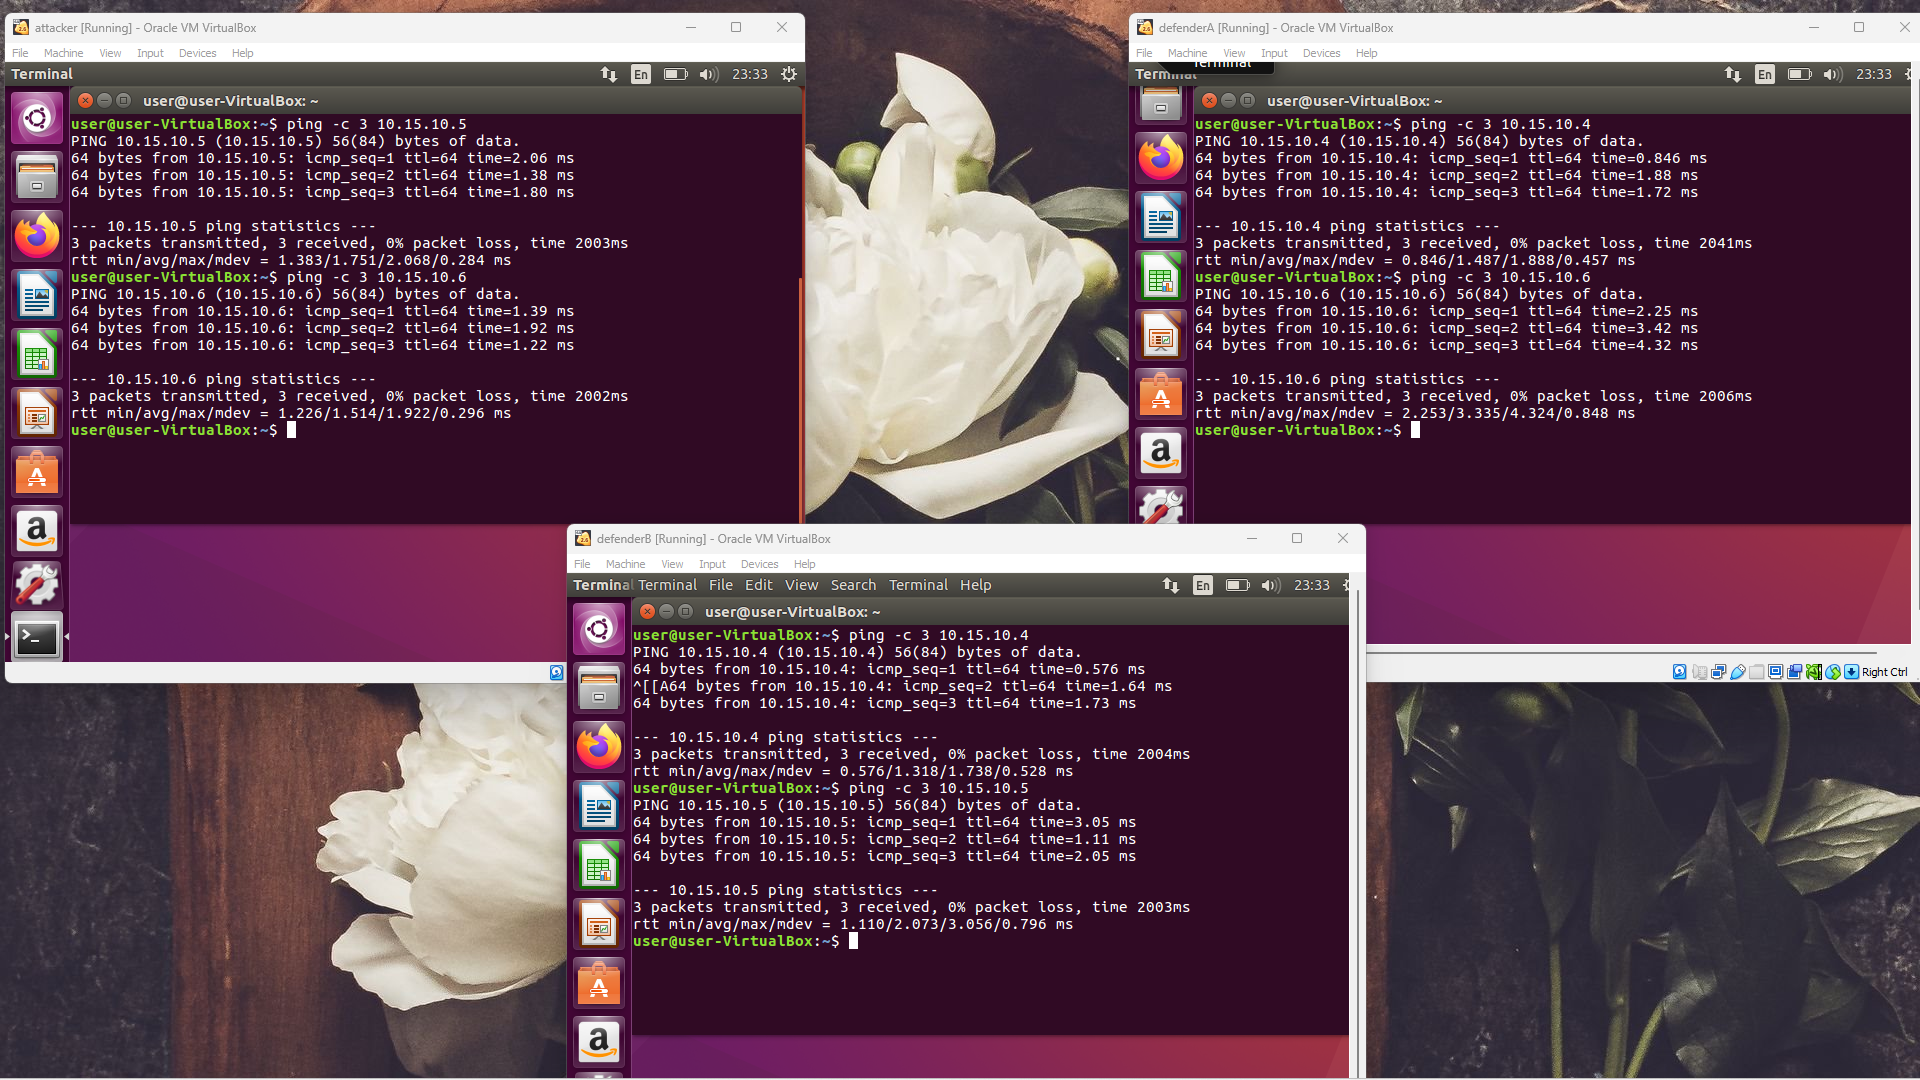
\includegraphics[width=0.85\textwidth]{02_00 (43)}
    \caption{Проверка доступности машин}
    \label{img:0032}
  \end{figure}

  Также рассмотрим текущее состояние \textit{ARP} таблиц для каждой из машин при помощи
  утилиты \textit{arp}:

  \begin{figure}[H]
    \centering
    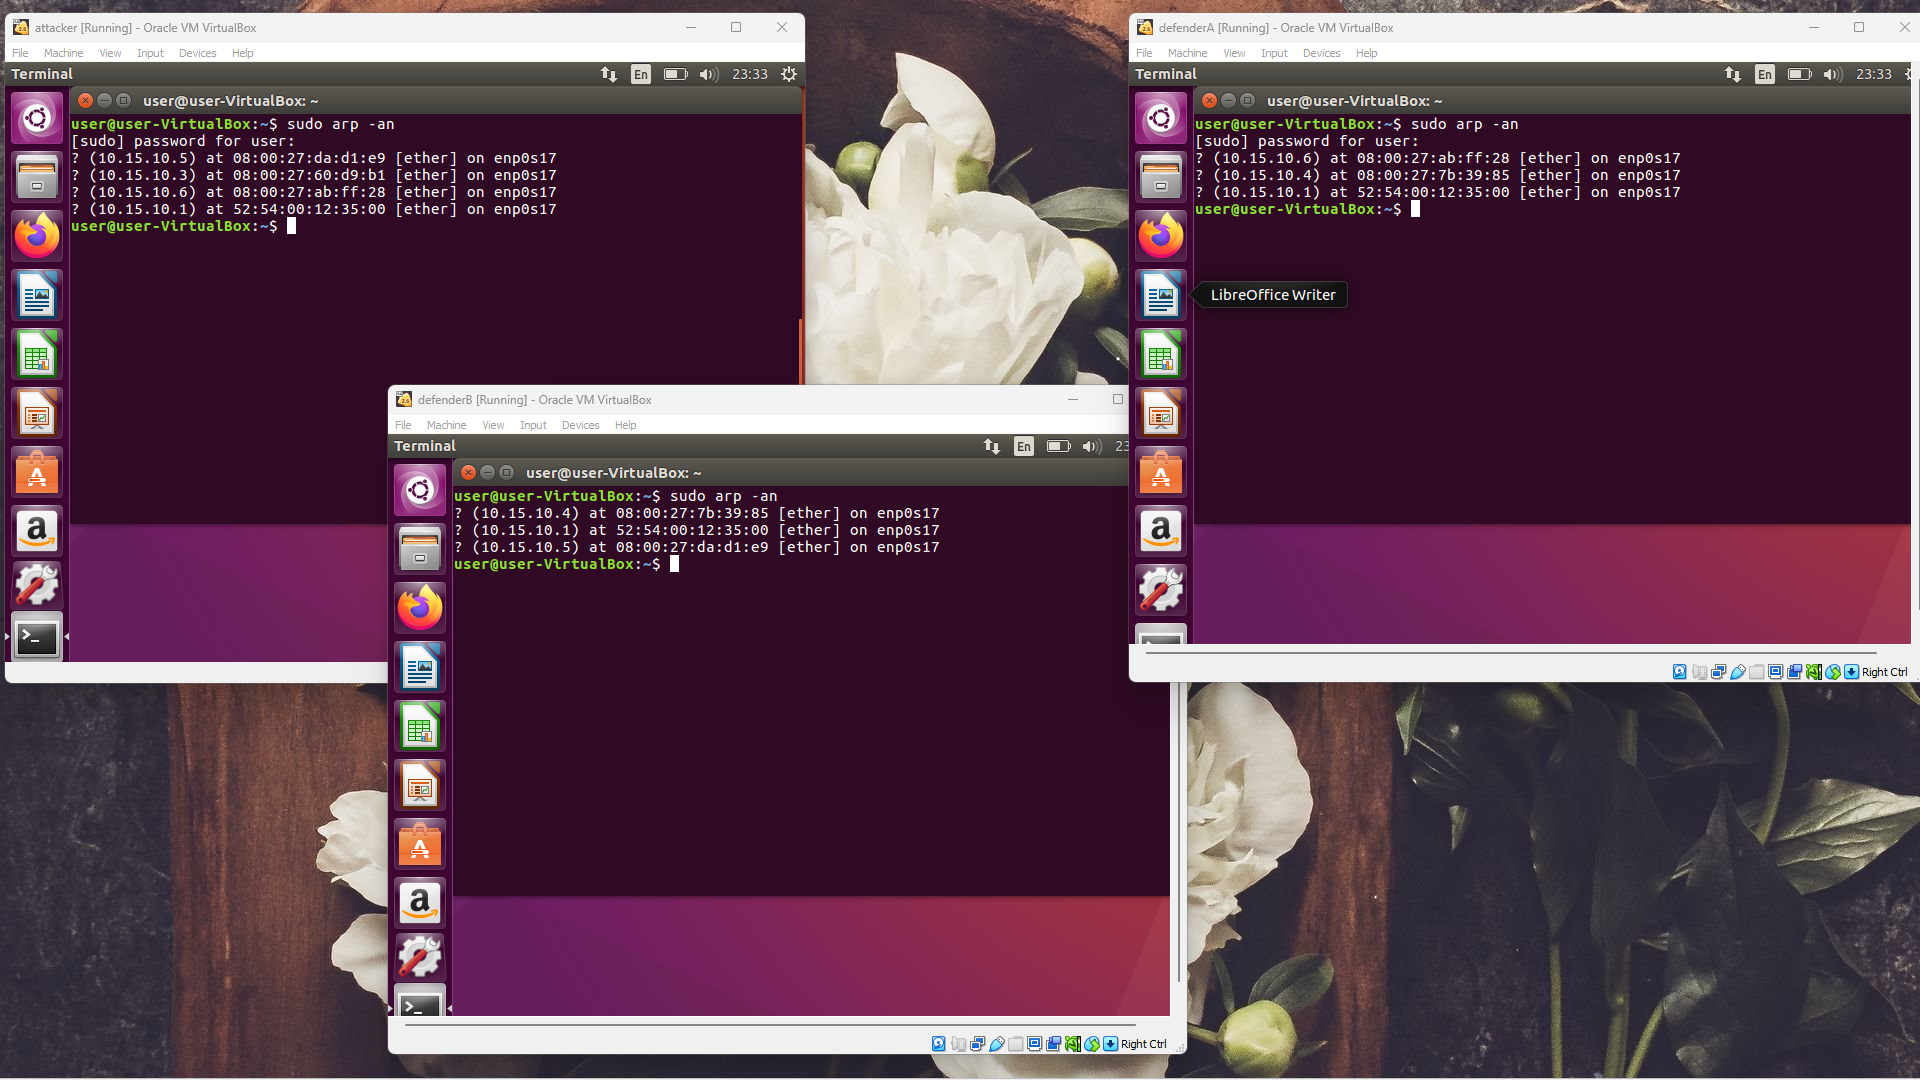
\includegraphics[width=0.85\textwidth]{02_00 (44)}
    \caption{sudo arp -an - результат запуска на каждой машине}
    \label{img:0033}
  \end{figure}

  Для того, чтобы лучше понять способ осуществления \textit{ARP} спуффинга, запустим
  сниффер для анализа трафика:

  \begin{figure}[H]
    \centering
    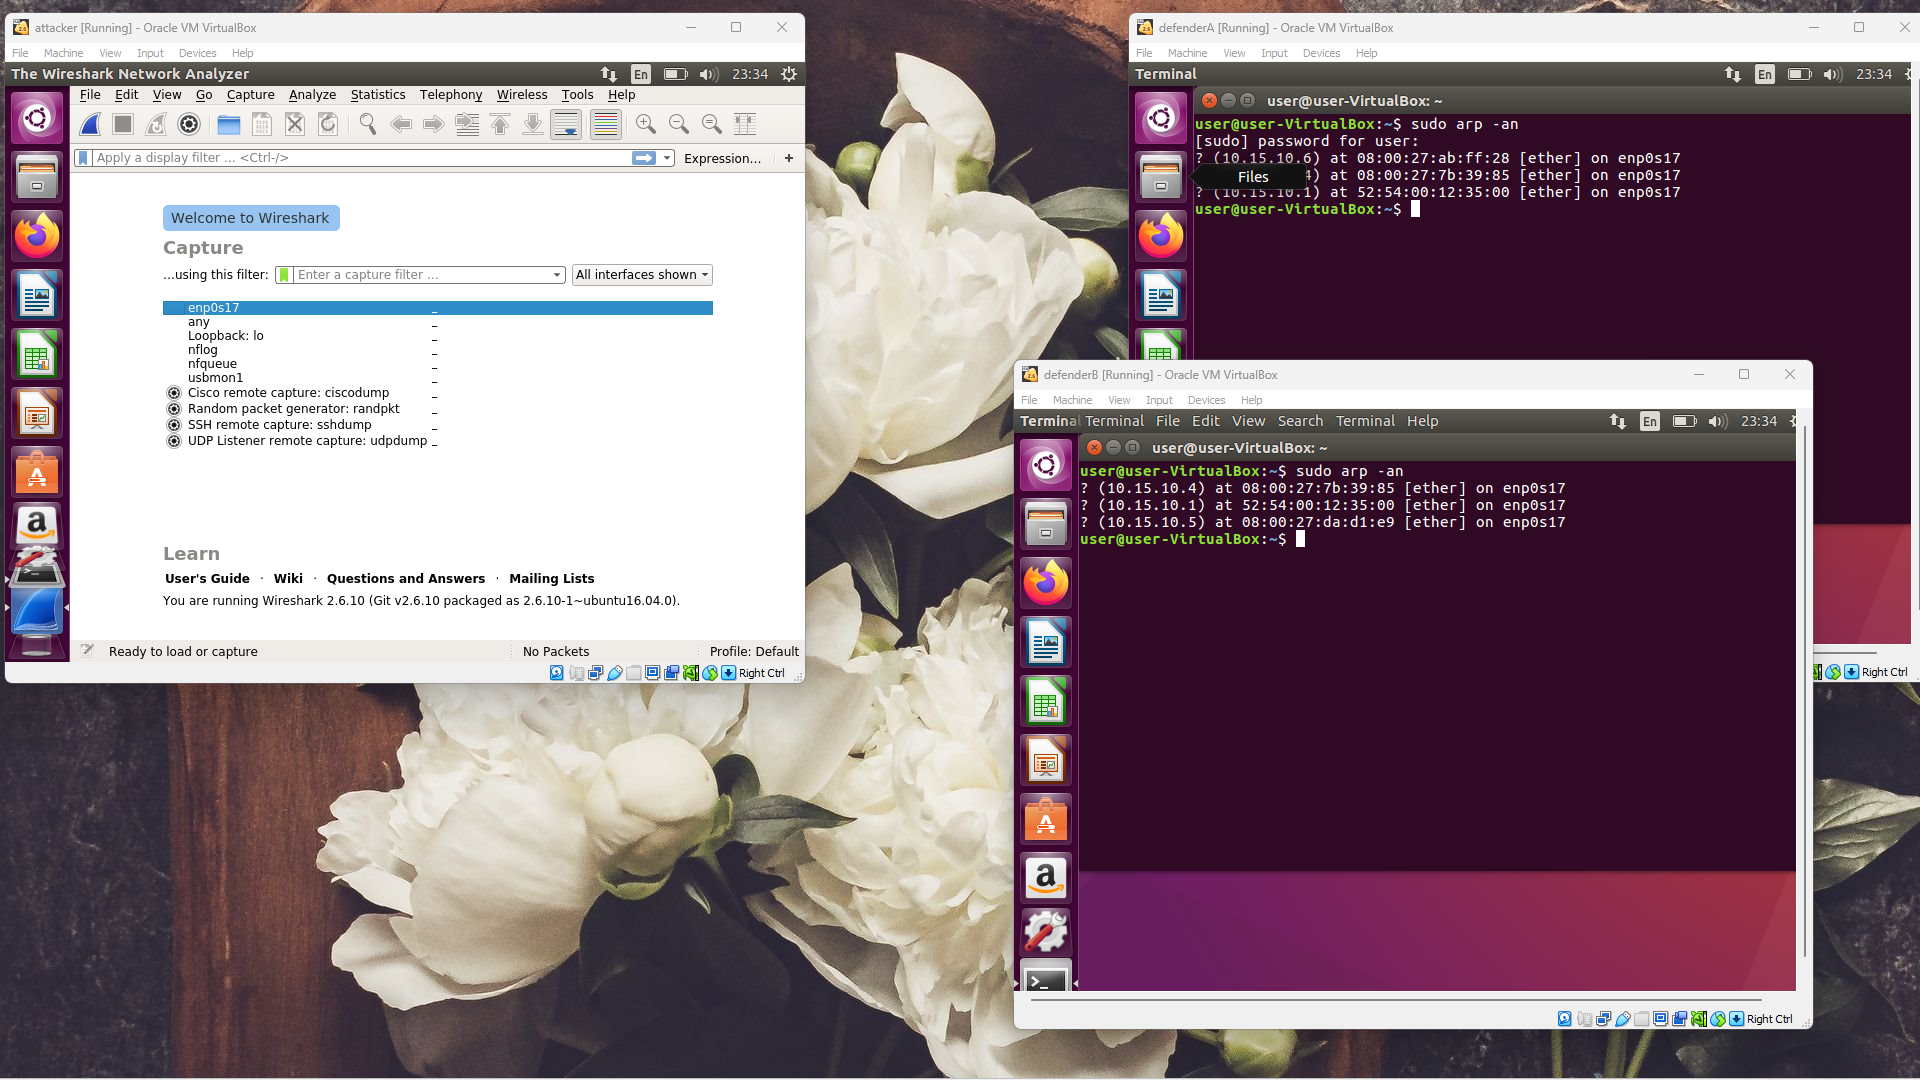
\includegraphics[width=0.85\textwidth]{02_00 (45)}
    \caption{Запускаем Wireshark}
    \label{img:0034}
  \end{figure}

  Чтобы анализировать только \textit{ARP} и \textit{ICMP} пакеты воспользуемся фильтром:

  \begin{figure}[H]
    \centering
    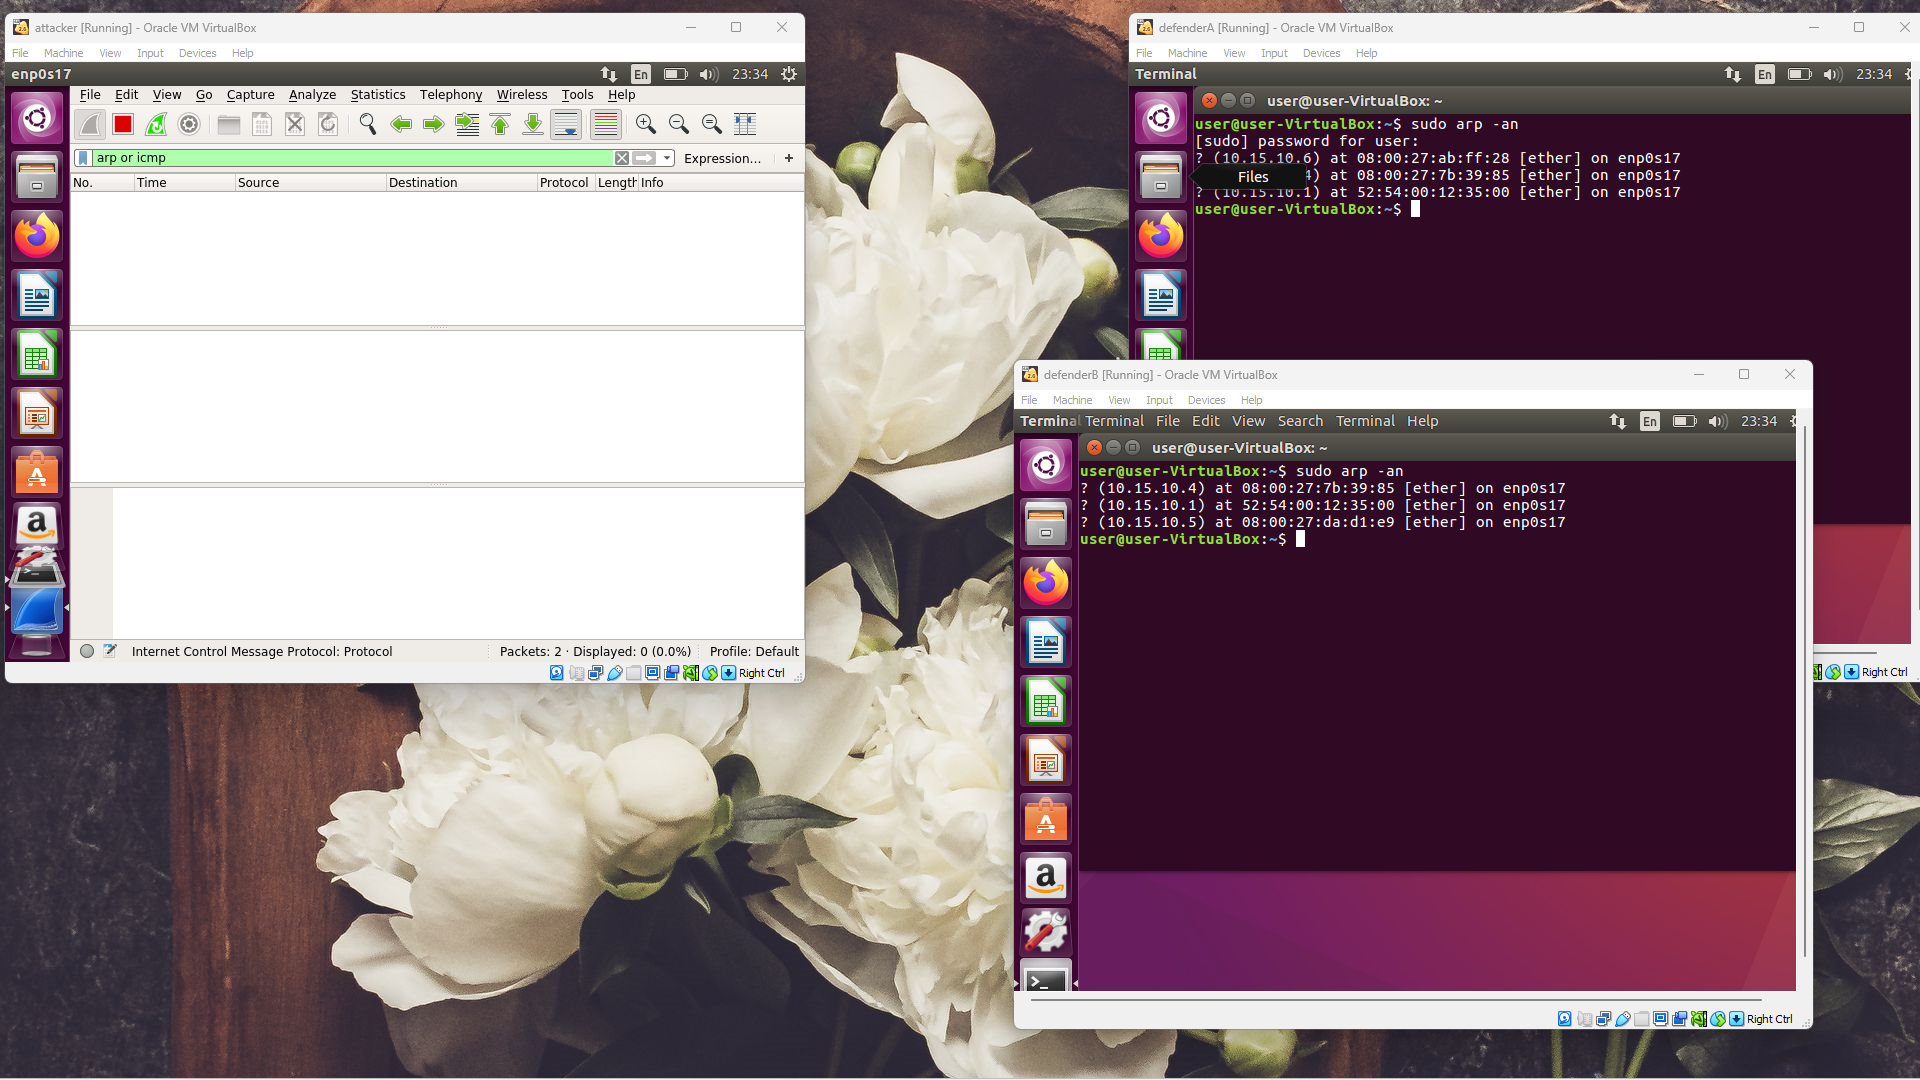
\includegraphics[width=0.85\textwidth]{02_00 (46)}
    \caption{Применяем подходящий фильтр}
    \label{img:0035}
  \end{figure}

  \subsubsection{Осуществление атаки}

  Для осуществления атаки снова запустим \textit{ettercap}:

  \begin{figure}[H]
    \centering
    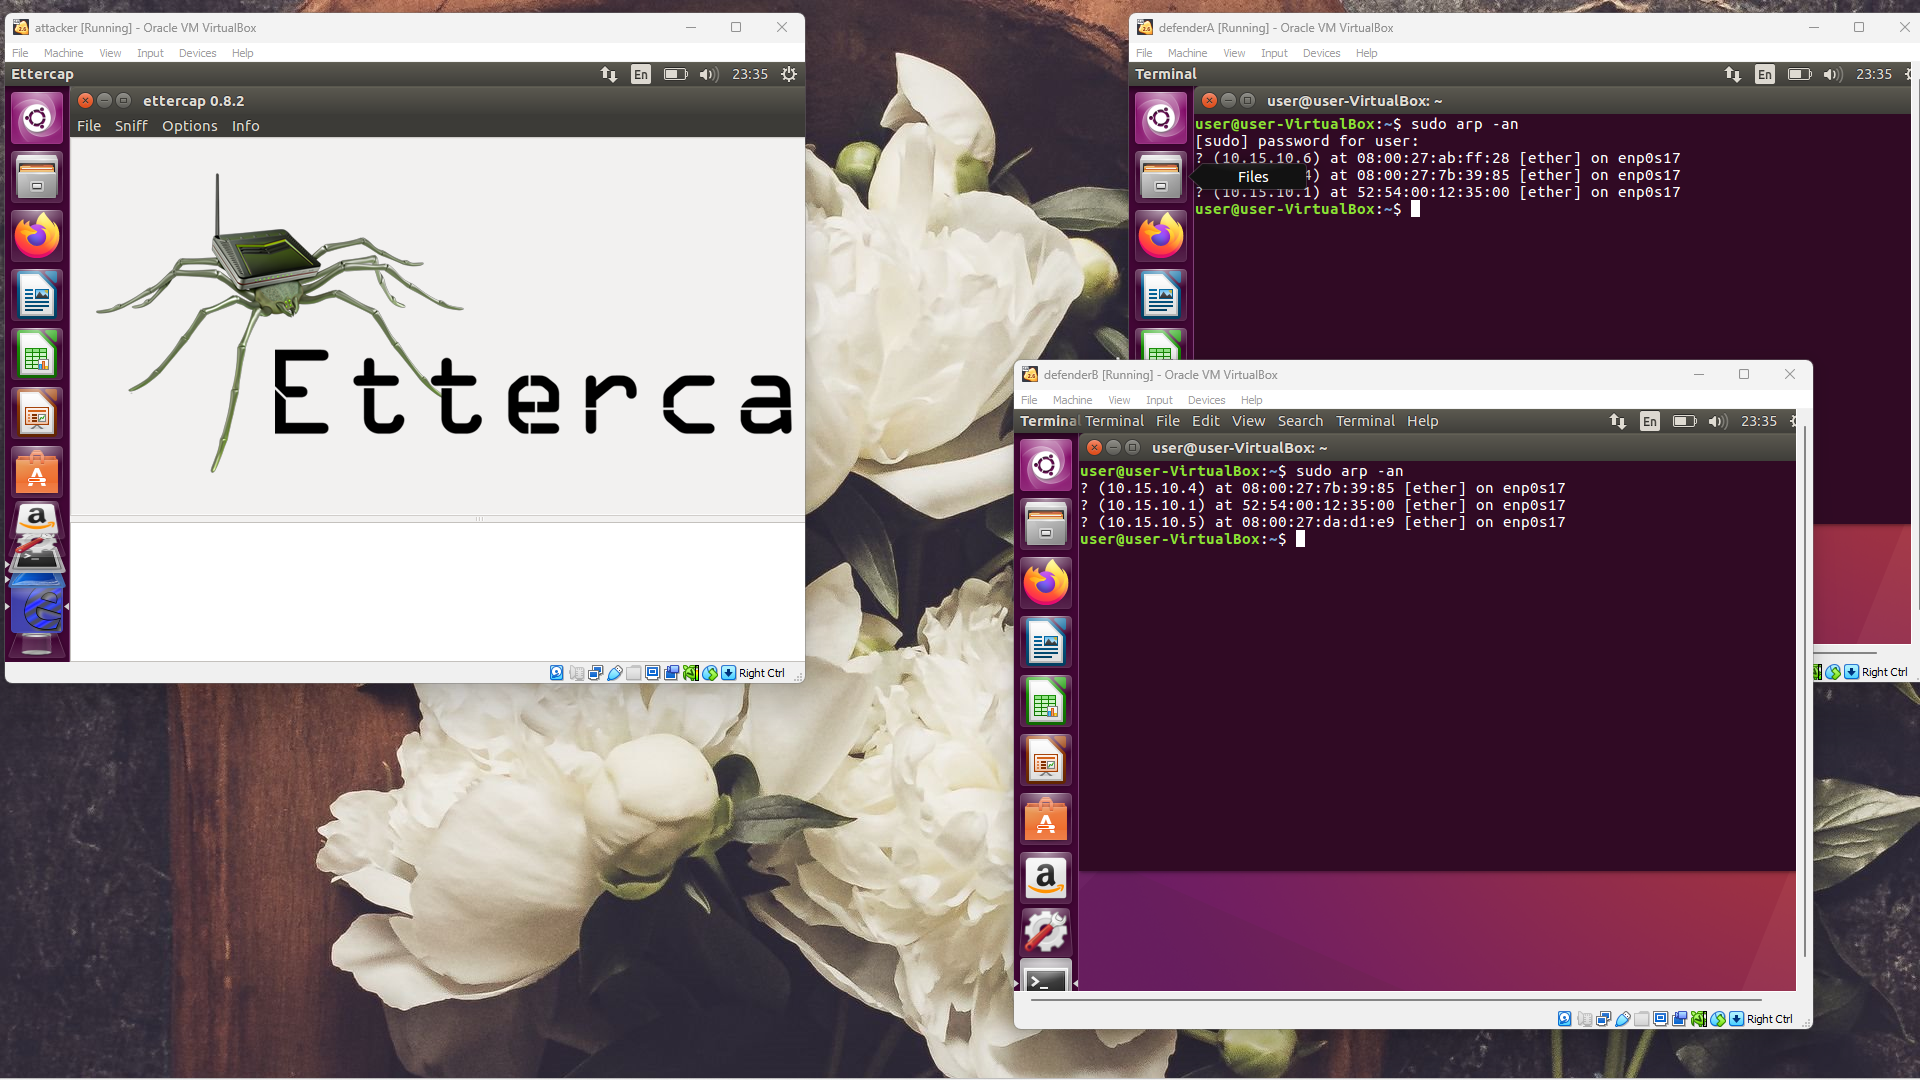
\includegraphics[width=0.85\textwidth]{02_00 (47)}
    \caption{Запушенный ettercap}
    \label{img:0036}
  \end{figure}

  Далее снова установим необходимый режим встроенного сниффера (см. предыдущую атаку) и просканируем
  сеть - изучим существующие хосты, для этого в меню \textbf{Hosts} выберем опцию \textbf{Scan for hosts}:

  \begin{figure}[H]
    \centering
    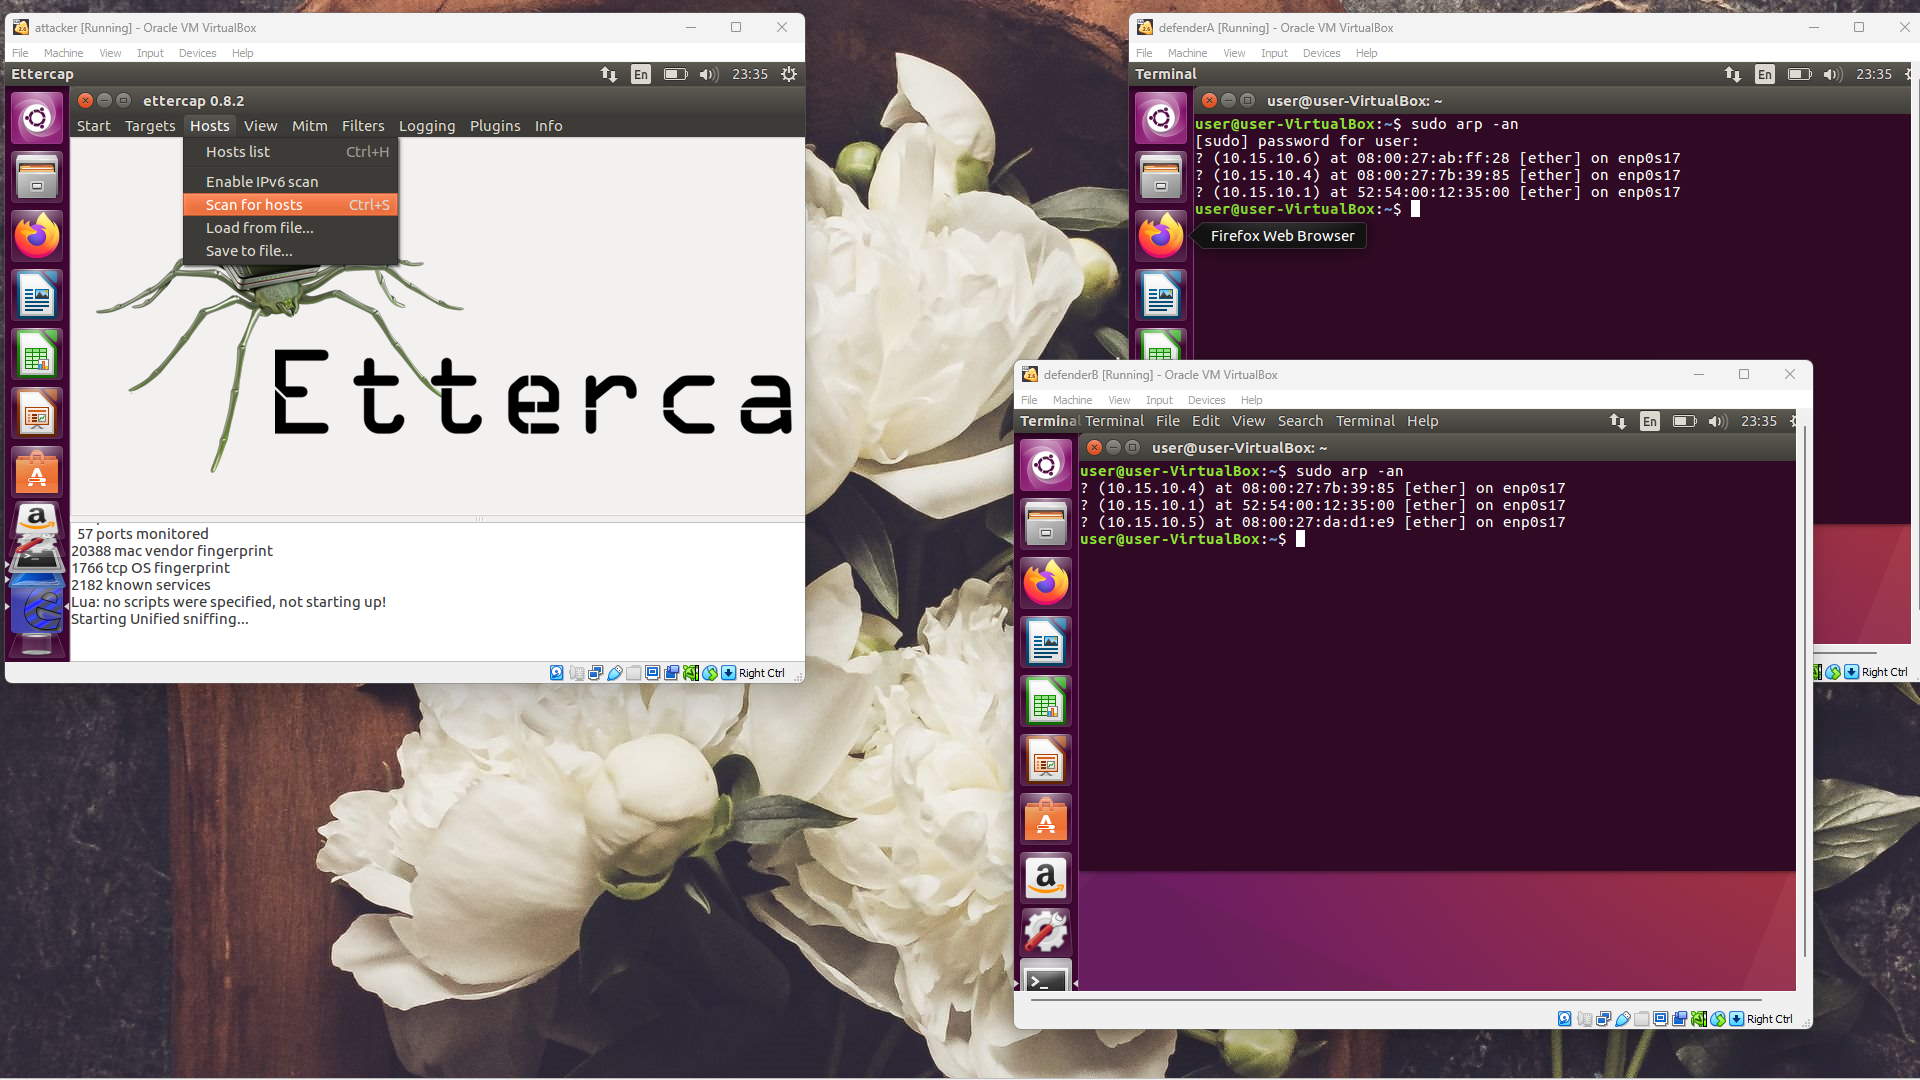
\includegraphics[width=0.85\textwidth]{02_00 (50)}
    \caption{Полученные информации о других машинах, находящихся в той же сети}
    \label{img:0037}
  \end{figure}

  \textit{ettercap} в своем окне отобразил, что просканировал 63 хоста, на 5 из которых 
  были обнаружены работающие устройства:

  \begin{figure}[H]
    \centering
    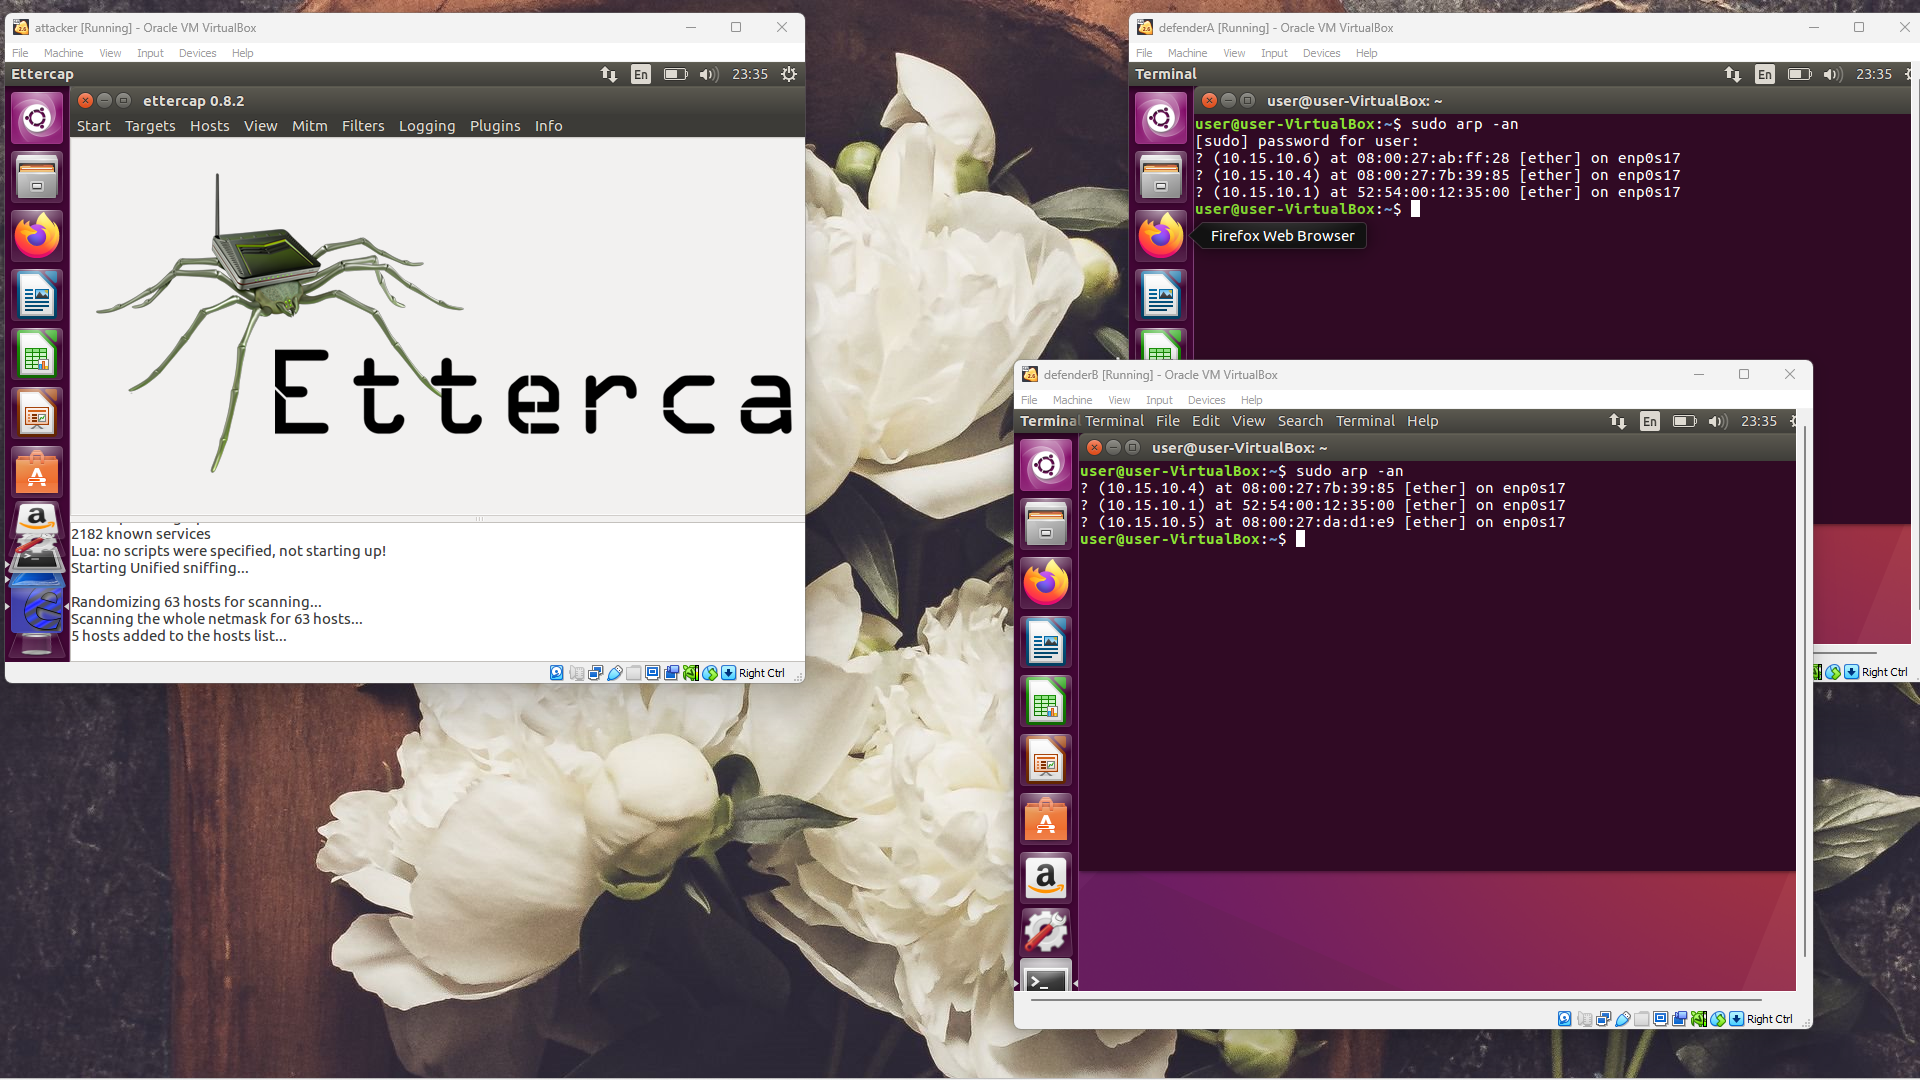
\includegraphics[width=0.85\textwidth]{02_00 (51)}
    \caption{Результат сканирования хостов}
    \label{img:0038}
  \end{figure}

  Далее укажем, между какими устройствами мы хотим стать посредником. Для этого в меню \textbf{Hosts}
  выбираем пункт \textbf{Host List}:

  \begin{figure}[H]
    \centering
    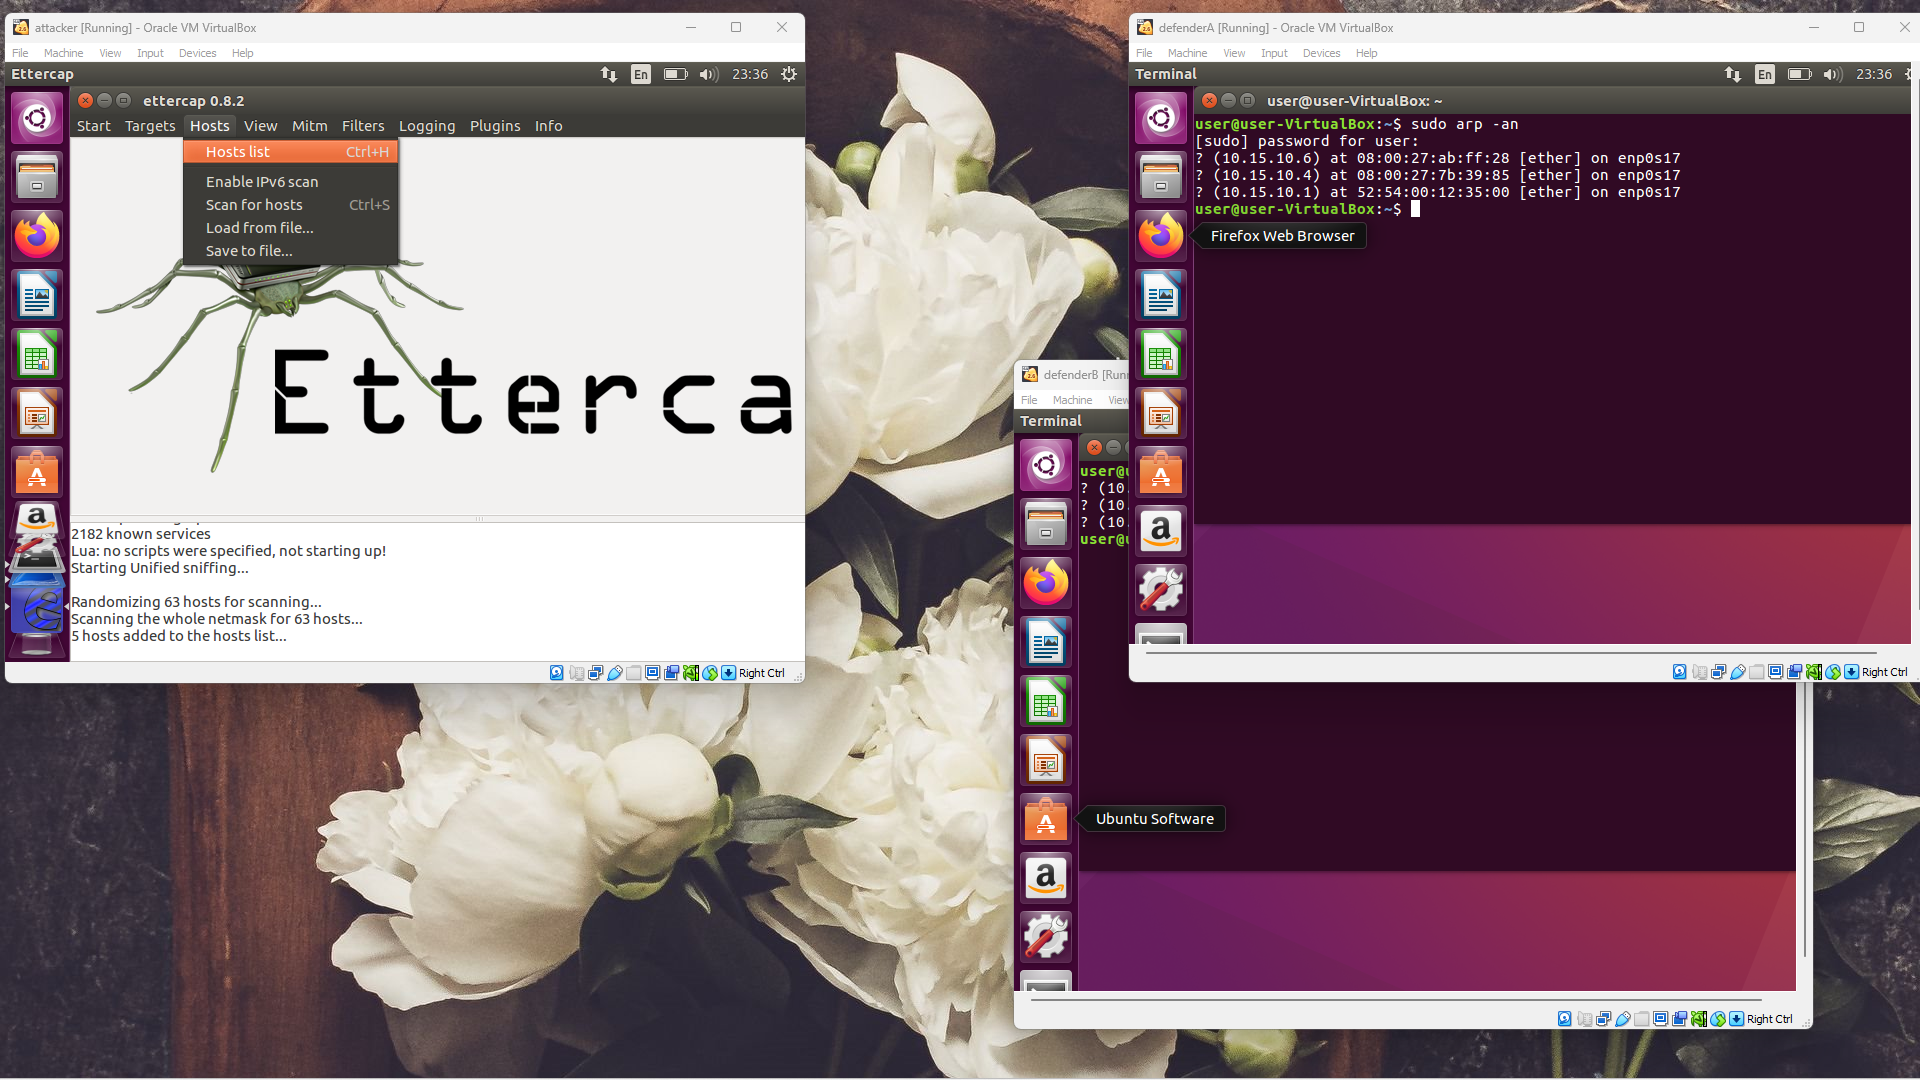
\includegraphics[width=0.85\textwidth]{02_00 (52)}
    \caption{Настраиваем спуффинг}
    \label{img:0039}
  \end{figure}

  В качестве первого адреса (target 1) указываем машину \textit{DefenderA} (10.15.10.5), а 
  в качестве второго (target 2) - \textit{DefenderB} (10.15.10.6):

  \begin{figure}[H]
    \centering
    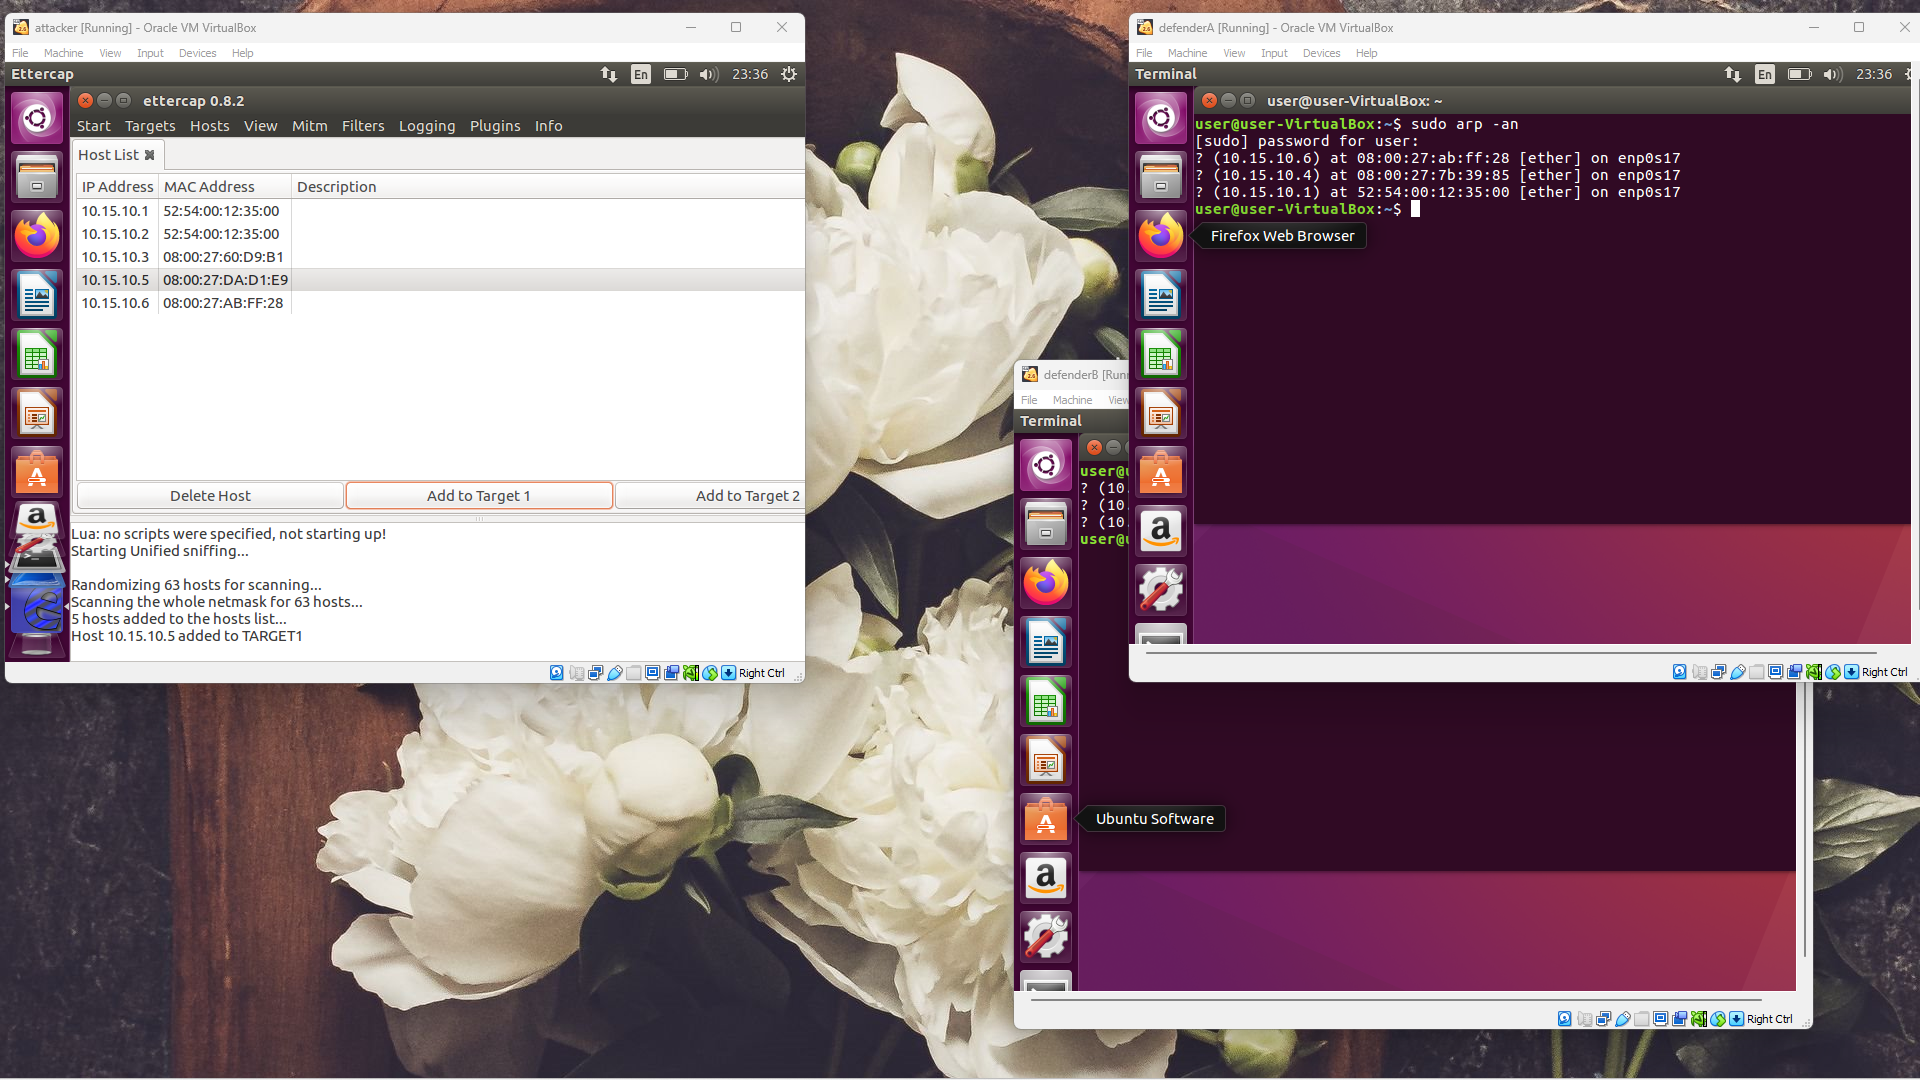
\includegraphics[width=0.85\textwidth]{02_00 (53)}
    \caption{Указываем первую цель}
    \label{img:0040}
  \end{figure}

  \begin{figure}[H]
    \centering
    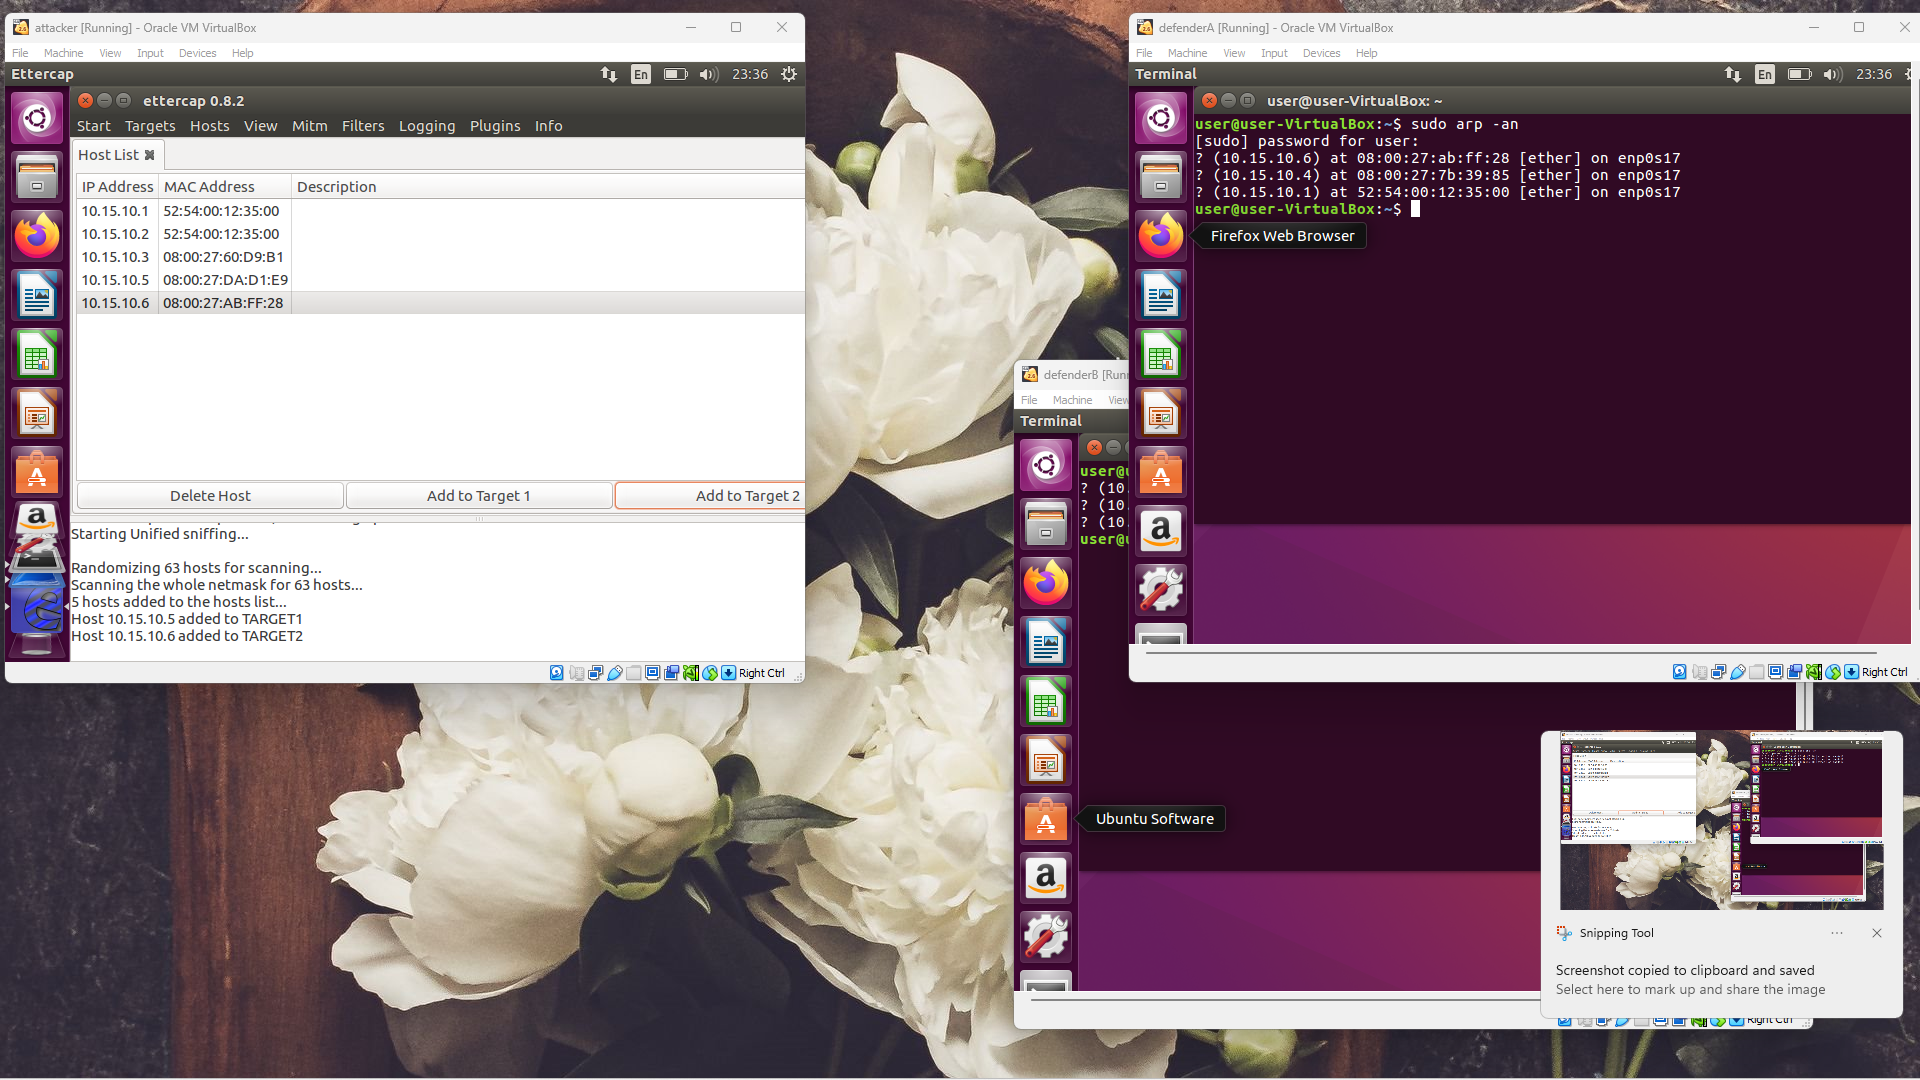
\includegraphics[width=0.85\textwidth]{02_00 (54)}
    \caption{Указываем вторую цель}
    \label{img:0041}
  \end{figure}

  Когда все настройки установлены, запускаем отравление \textit{ARP} кеша,
  для этого в меню \textbf{Mitm} выбираем пункт \textbf{ARP Poisoning}:

  \begin{figure}[H]
    \centering
    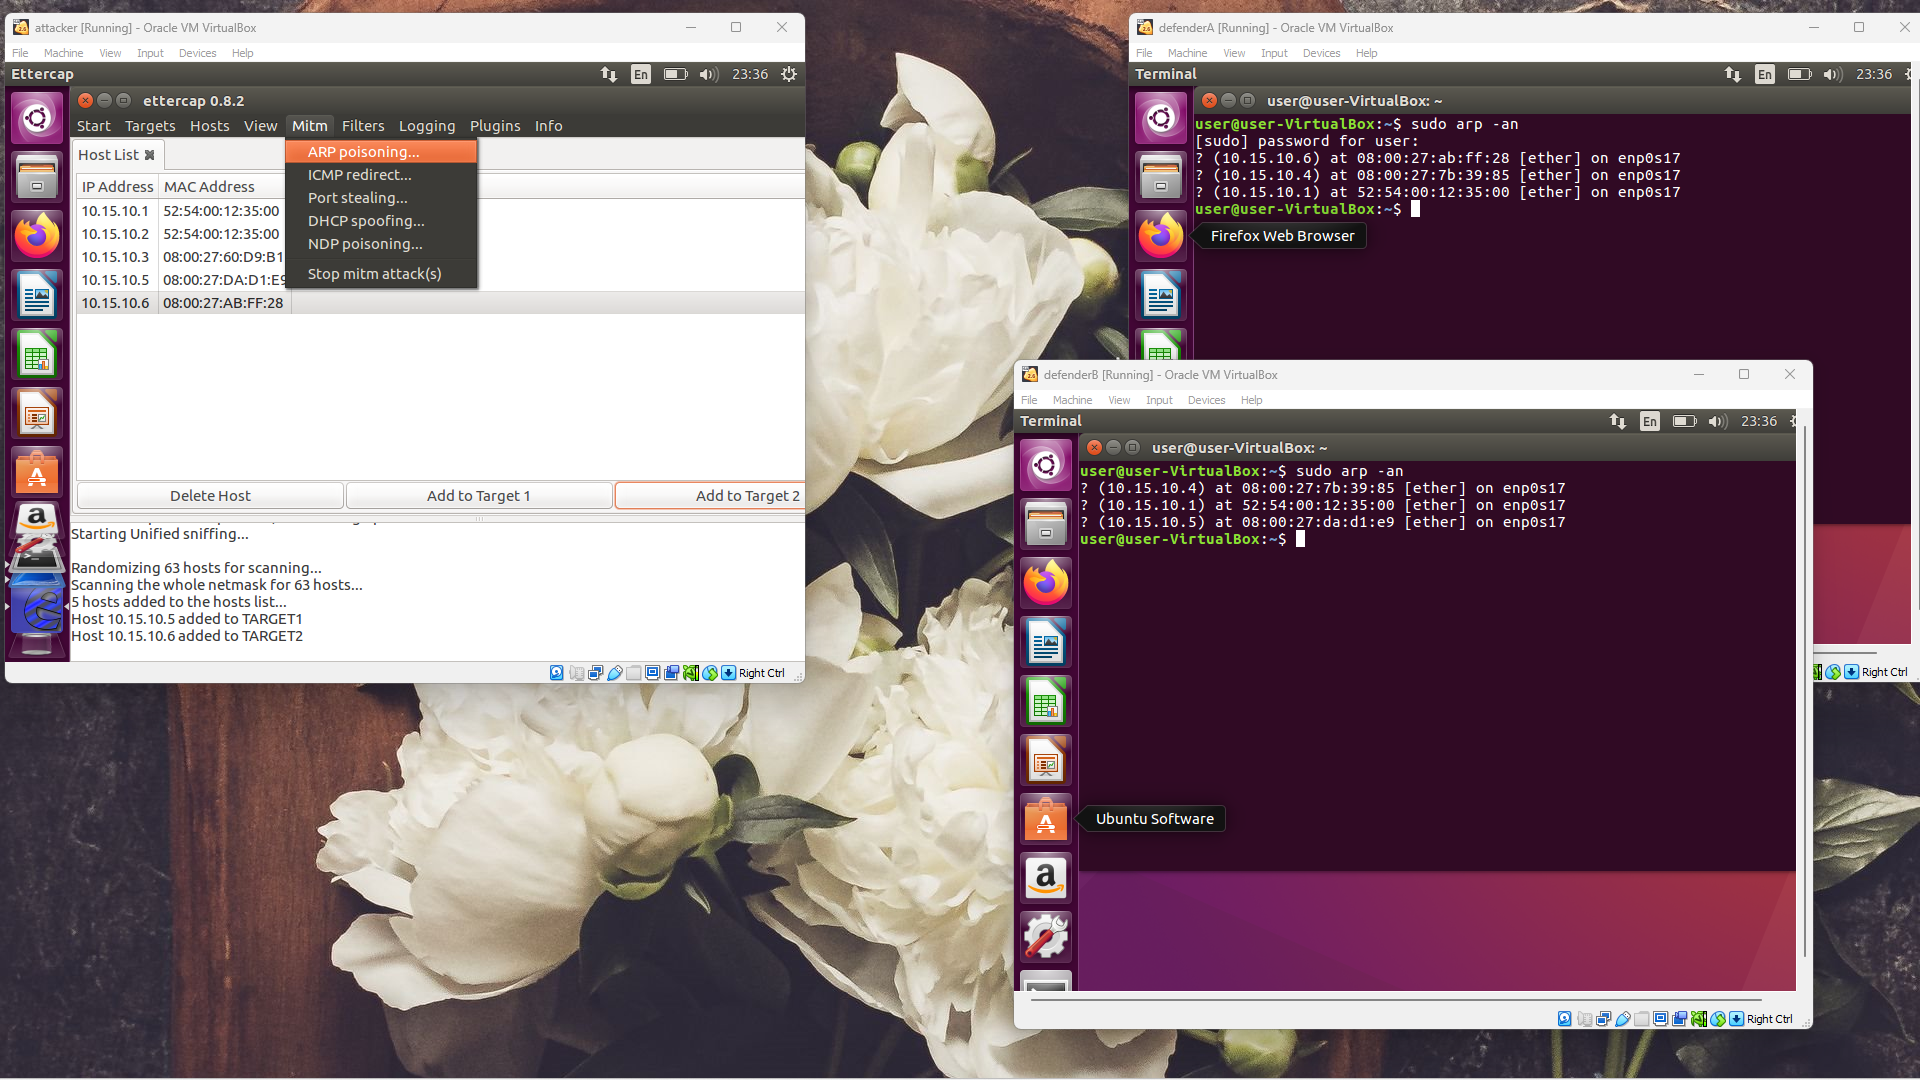
\includegraphics[width=0.85\textwidth]{02_00 (55)}
    \caption{Запуск атаки}
    \label{img:0042}
  \end{figure}

  \begin{figure}[H]
    \centering
    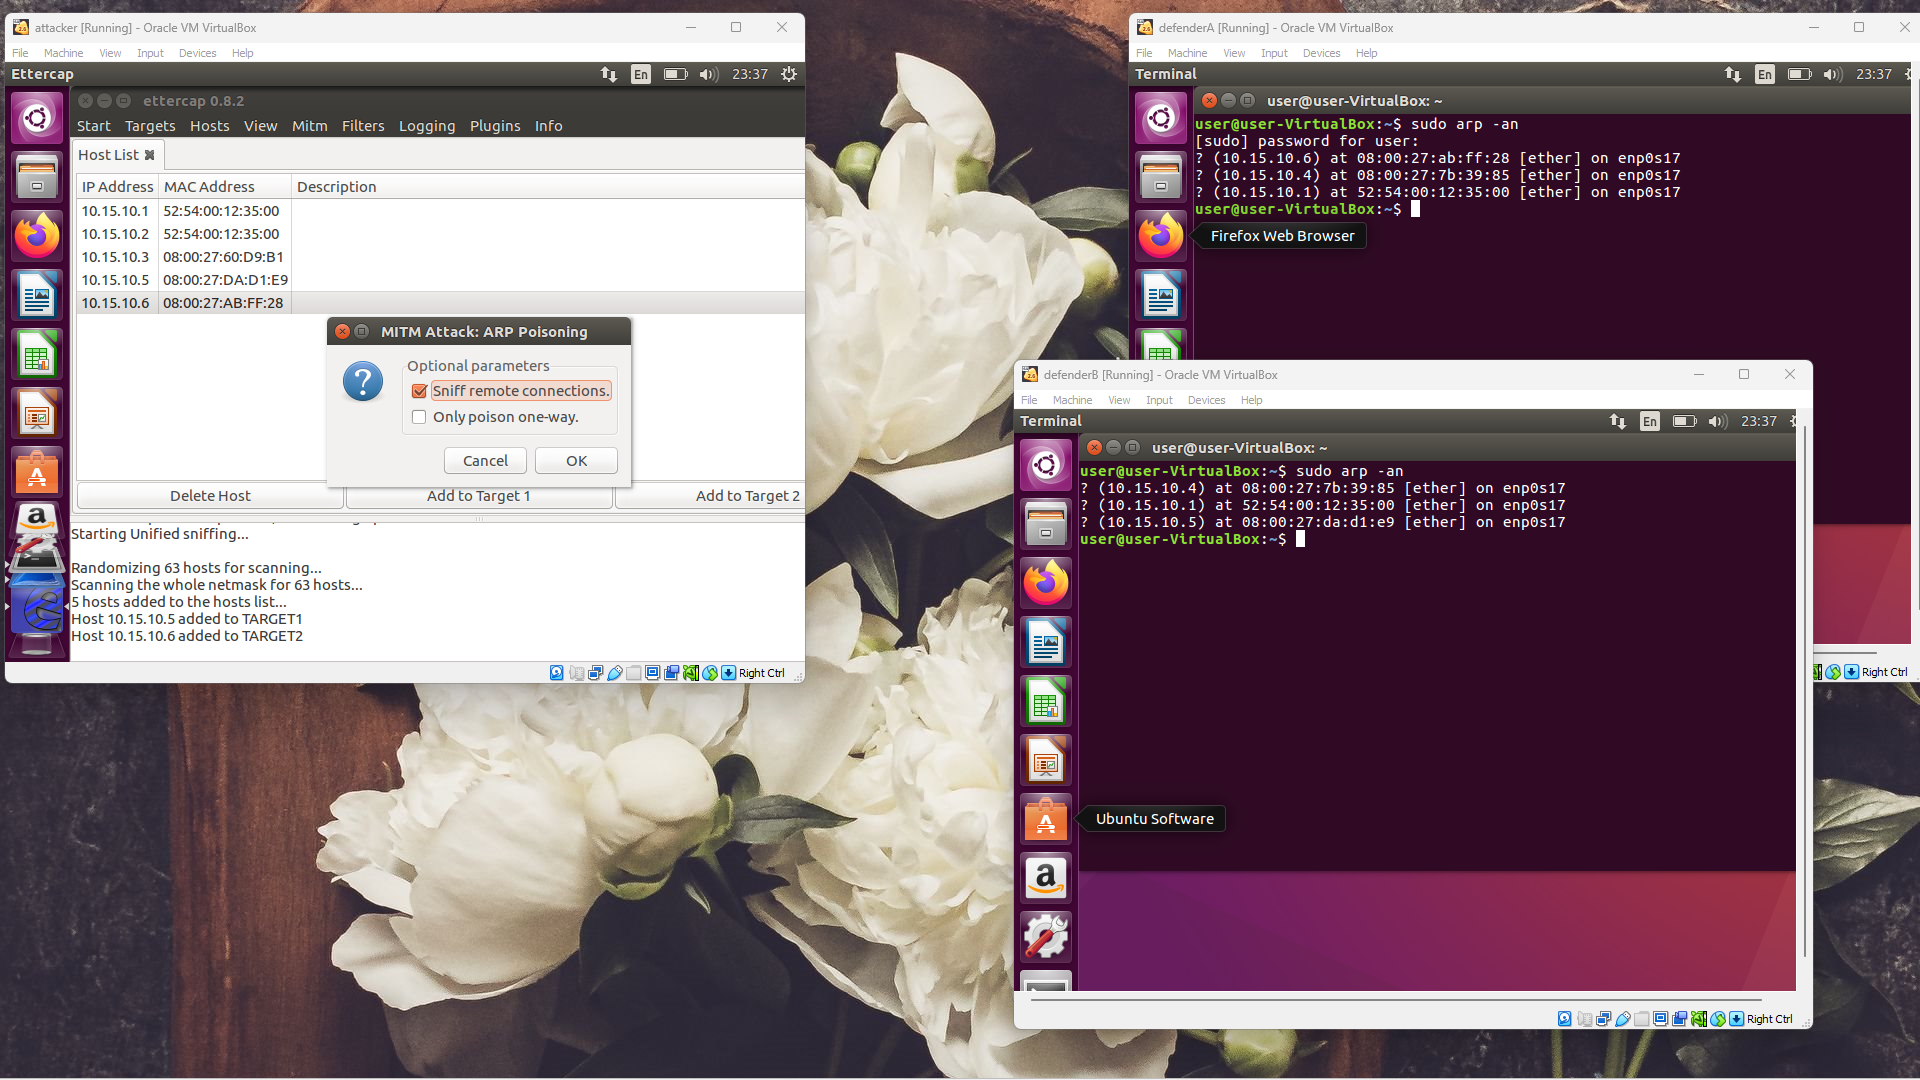
\includegraphics[width=0.85\textwidth]{02_00 (56)}
    \caption{Атакуем все удаленные соединения}
    \label{img:0043}
  \end{figure}

  После нажатия кнопки \textbf{OK} \textit{ARP} кеш был отравлен, посмотрим, что изменилось
  в \textit{ARP} таблицах виртуальных машин:

  \begin{figure}[H]
    \centering
    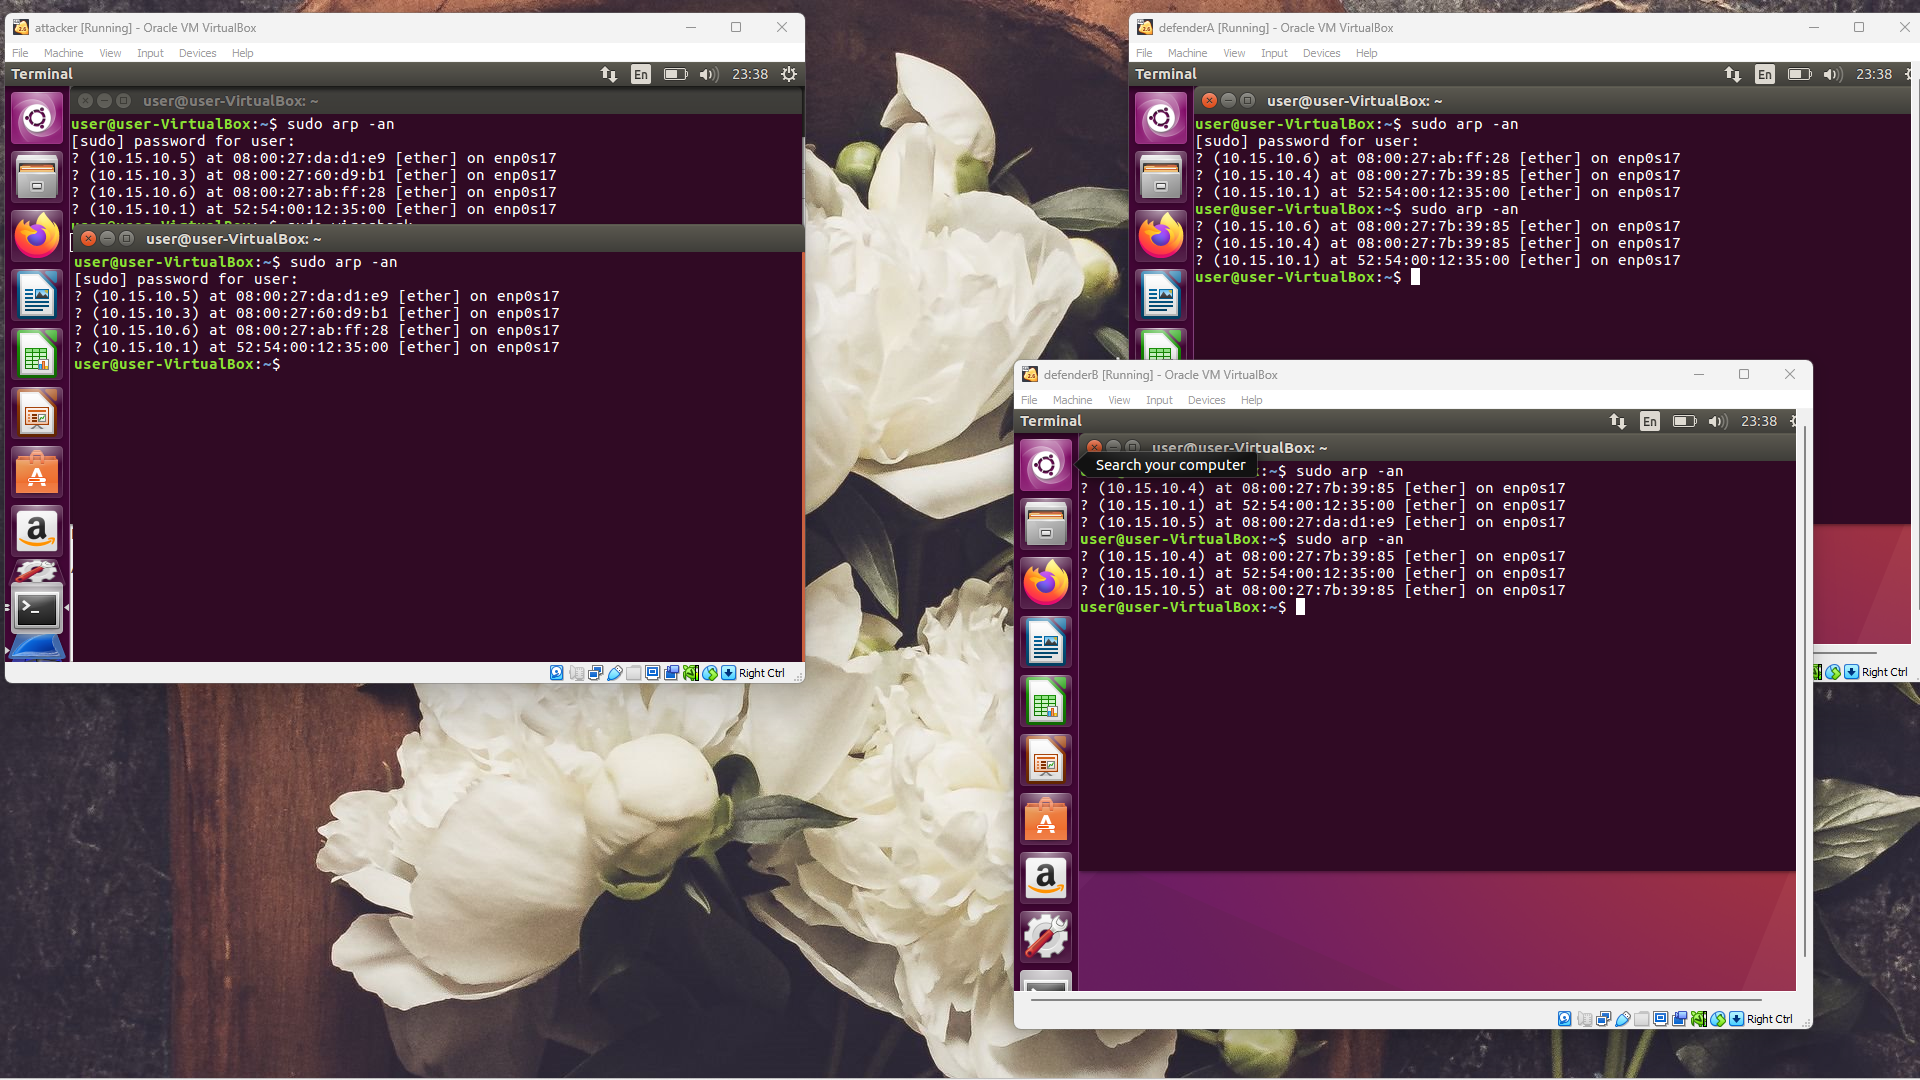
\includegraphics[width=0.85\textwidth]{02_00 (57)}
    \caption{Новые ARP таблицы}
    \label{img:0044}
  \end{figure}

  Здесь можно увидеть, что атака удалась. В частности, до осуществления атаки, если машина 
  \textit{DefenderA} (10.15.10.5) отправляла пакет на \textit{DefenderB} (10.15.10.6),
  то она отправляла его на реальный \textit{MAC} адрес \textit{DefenderB}.
  После отравления \textit{ARP} кеша отправка по факту осуществляется на \textit{MAC} адрес \textit{Attacker},
  что позволяет злоумышленнику перехватывать информацию.

  Ситуация абсолютно аналогична для отправки пакетов с \textit{DefenderB} на \textit{DefenderA}.

  Изучим перехваченный трафик:

  \begin{figure}[H]
    \centering
    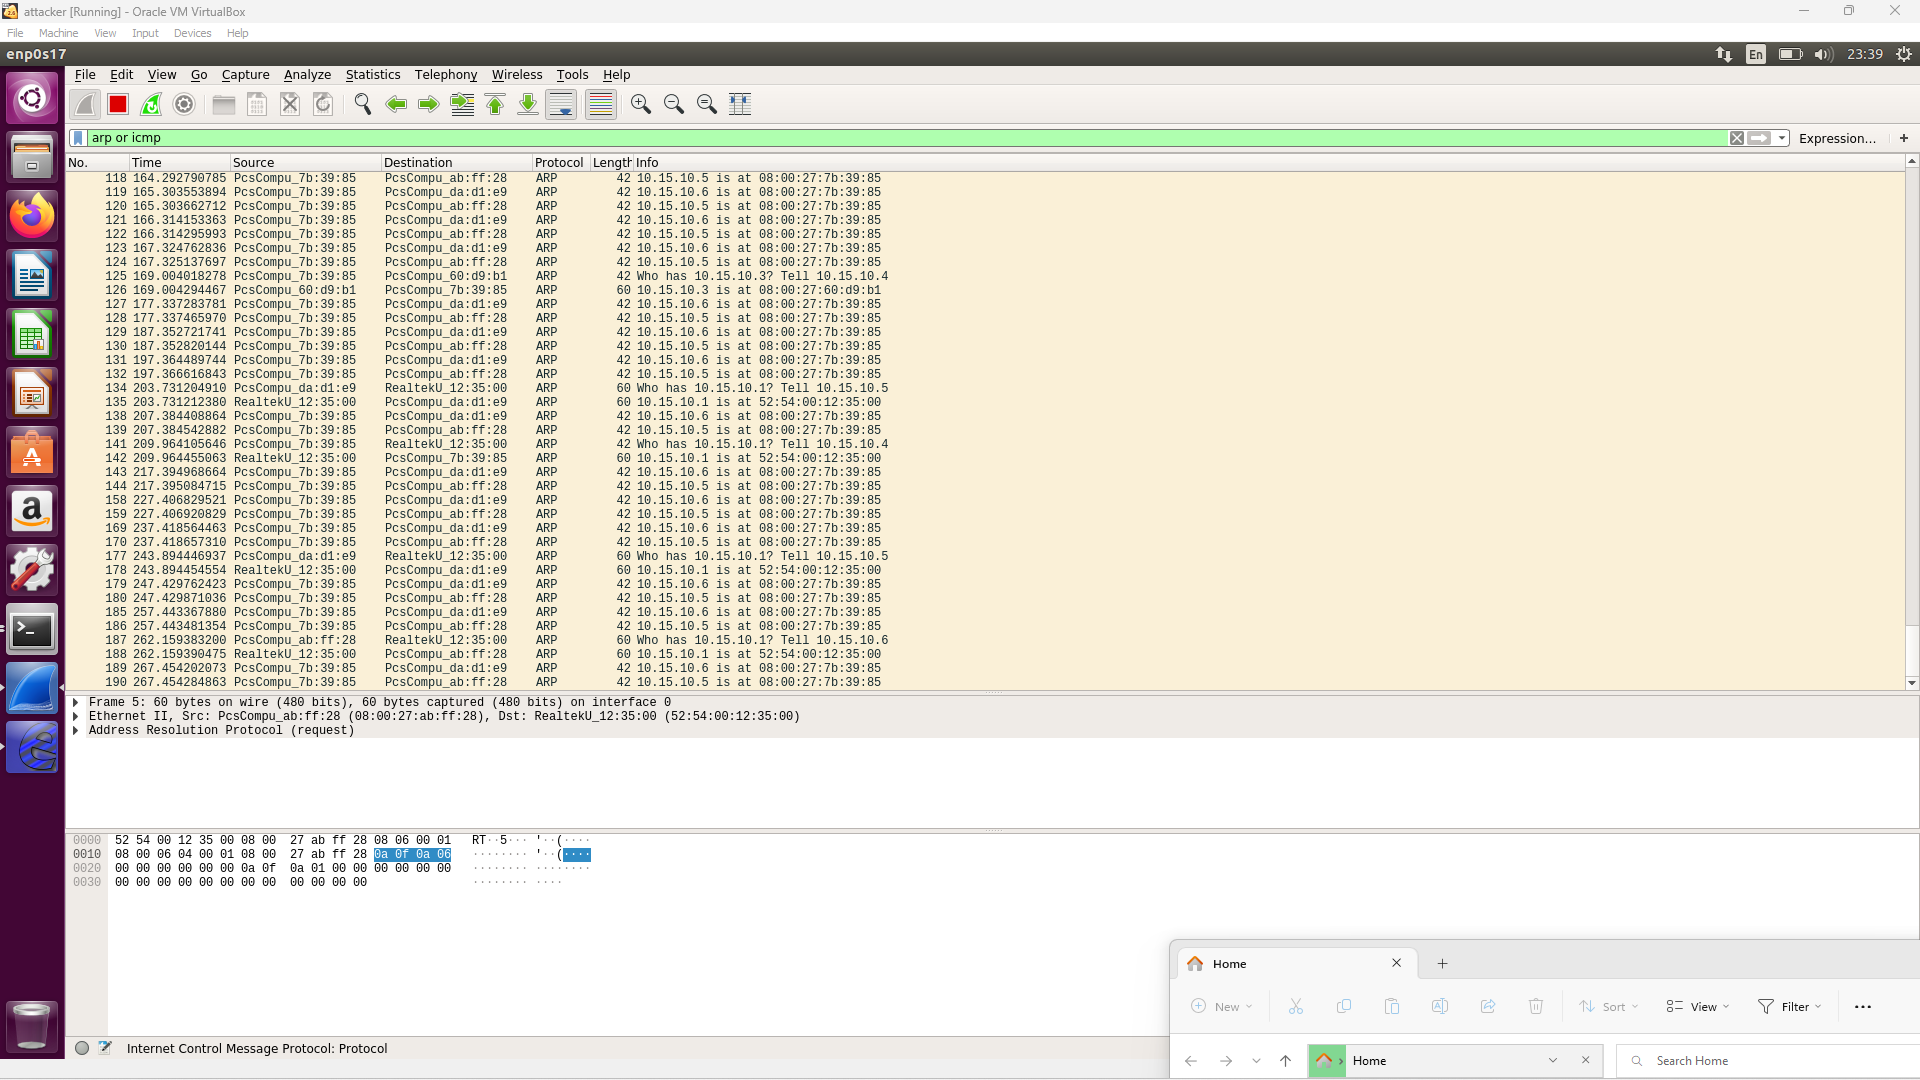
\includegraphics[width=0.85\textwidth]{02_00 (58)}
    \caption{Захваченные пакеты}
    \label{img:0045}
  \end{figure}

  Видно, что захваченно очень много \textit{ARP} пакетов, указывающих неправильную информацию. То
  есть суть \textit{ARP} спуффинга заключается в очень частом отравлении \textit{ARP} кеша, перехвате пакетов
  и эмулияции реального соединения между маштинами - по факту атака вида \textit{Man In The Middle}.

  Теперь попробуем остановить атаку и посмотреть, вернется ли все в норму:
  
  \begin{figure}[H]
    \centering
    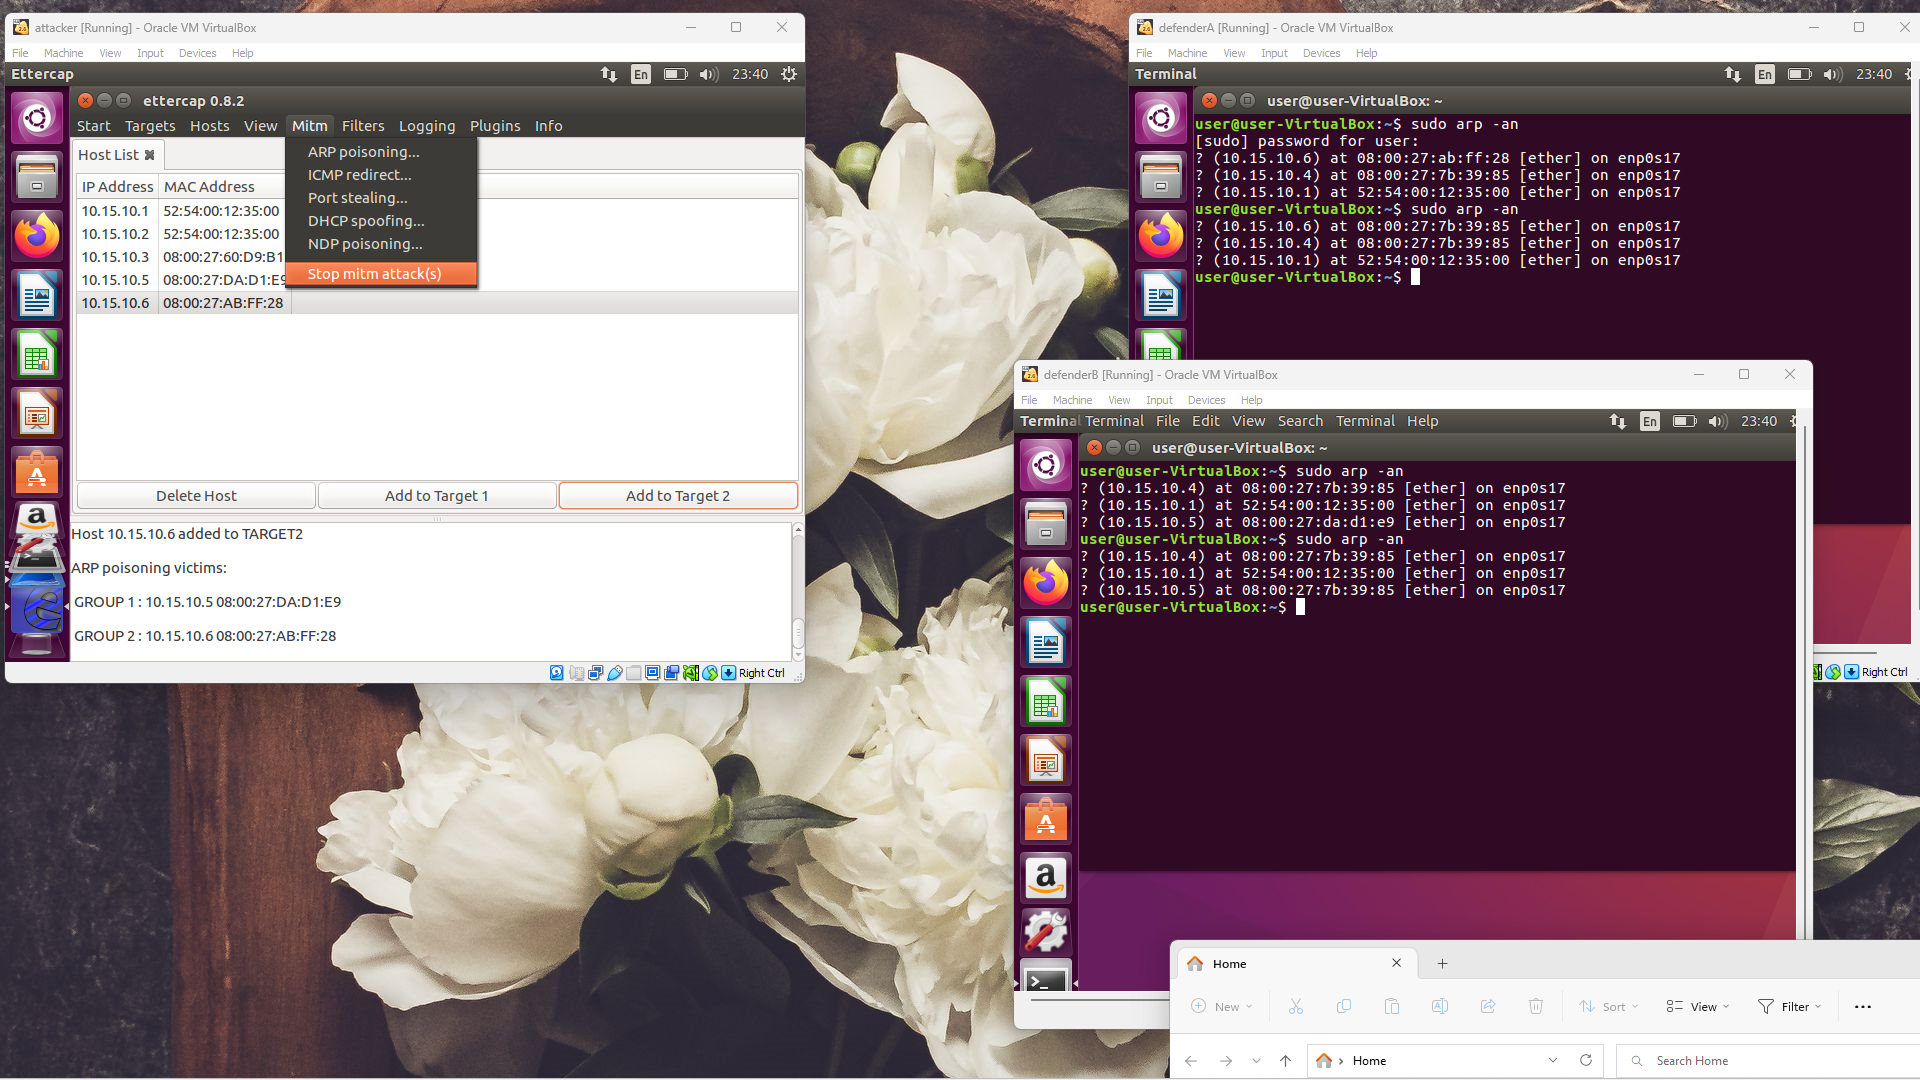
\includegraphics[width=0.85\textwidth]{02_00 (60)}
    \caption{Остановка отравления ARP кеша}
    \label{img:0046}
  \end{figure}
  
  \begin{figure}[H]
    \centering
    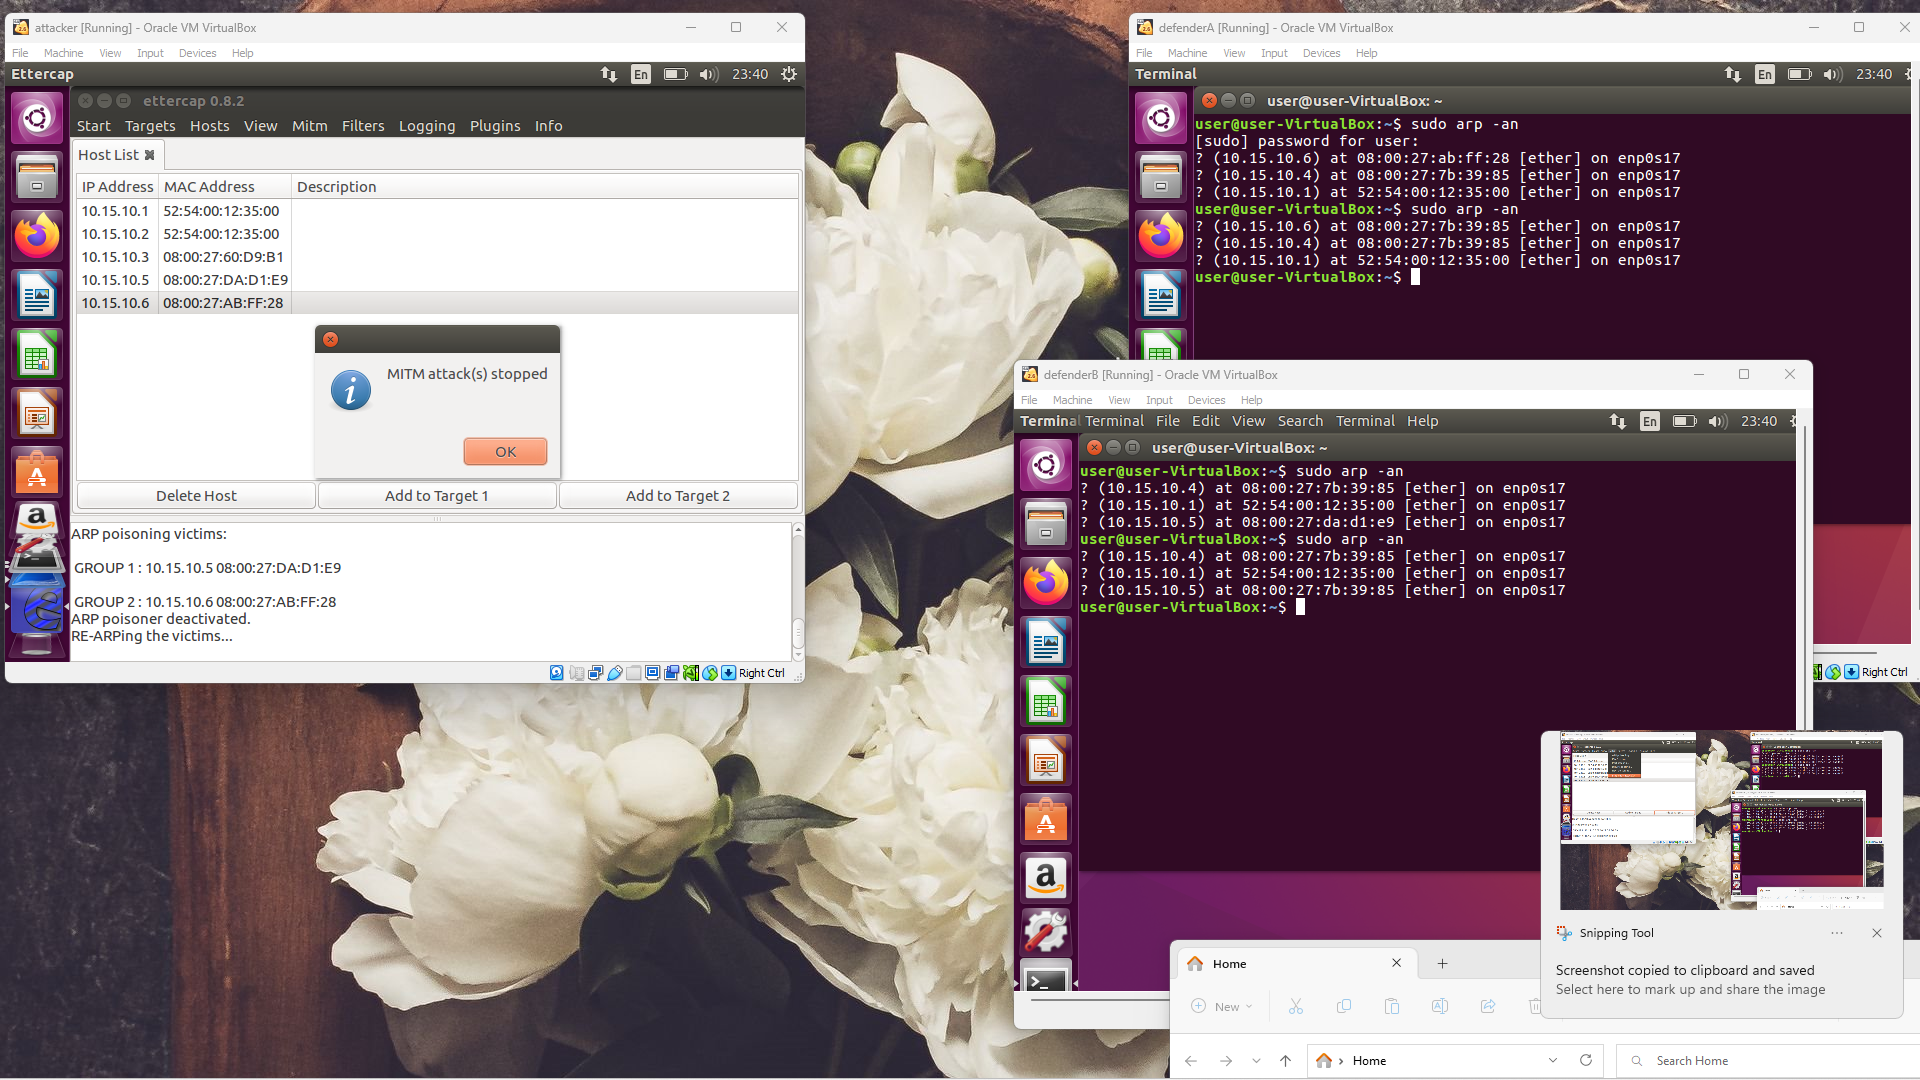
\includegraphics[width=0.85\textwidth]{02_00 (61)}
    \caption{Новые ARP таблицы}
    \label{img:0047}
  \end{figure}

  После остановки атаки все \textit{ARP} таблицы вернулись к исходному состоянию,
  что говорит о том, что \textit{ARP} кеш очень краткосрочный и для успешной атаки
  необходимо очень часто его отравлять.

  \section{Вывод}

  В ходе данной работы мне удалось узнать, как изнутри работают \textit{DHCP} и \textit{ARP} спуффинг,
  как осуществить данные атаки и понять, что может послужить флагами для их обнаружения.

\end{document}

